\section{Results}
In the following, some test cases with CLSAdvection method are presented. It is known that the level set method can improve the sharpness of the interface but also cause mass loss. Whereas, the volume of fluid method keeps the interface mass conservative but smeared. Therefore, the validation of the CLSAdvection method is tested in this article's work and there are several simple cases comparing this coupled method with the level set method and volume of fluid method. The error measures will be used to quantify the solution quality with following aspects.\\
--- Volume conservation\\
In order to track the precision of the advection process, volume conservation is measured to testify whether the simulated results conform to Navier-Stokes equations' requirement. The fractional volume conservative error is defined as following equation by this article\cite{gopala2008volume},
\begin{equation}\label{28}
\varepsilon_{V}(t)=\frac{\left|\sum\limits^N_{i=1}\alpha_i(t)V_i-\sum\limits^N_{i=1}\alpha_i(0)V_i\right|}{\sum\limits^N_{i=1}\alpha_{i}(0)V_i}.
\end{equation}
--- Mass conservation\\
The introduction of level set method that can cause the loss of mass for using equation (\ref{16}) to define the density may underlie a slight mass loss. Nevertheless, the coupled method is aimed to improve the algorithm's ability of mass conservation, which is measured by the following equation,
\begin{equation}\label{29}
\varepsilon_{M}(t)=\frac{\left|\sum\limits^N_{i=1}\rho_i(t)V_i-\sum\limits_{i=1}^N\rho_i(0)V_i\right|}{\sum\limits^N_{i=1}\rho_i(0)V_i}.
\end{equation}
--- Sharpness\\
The interface is shaper, the width of the region where $\alpha$ changes from 0 to 1 is thinner. Therefore, the following equation measures the sharpness.
\begin{equation}\label{30}
\varepsilon_{S}(t)=\frac{\sum_j\alpha_j(t)V_j}{\sum_i\alpha_i(t)V_i},
\end{equation}
where $j$ means the cells where $0.01\leq\alpha_j(t)\leq{0.99}$.\\
--- Boundedness\\
Volume fractions need to be physically meaningful, which means the condition $0\leq\alpha\leq{1}$ should be met. The measures of boundedness is $\min{(\alpha)}$ and $\max{(\alpha)}$. The measurements are taken all over the domain at the end of the calculation.\\ 
--- Efficiency\\
Efficiency is measured by the simulation times $T_{calc}$. All the simulation were executed on a single core of an Intel$^{\textregistered}$ 2.80 GHz CPU(i7-7700HQ) on a Dell$^{\textregistered}$ Precision 3520 Mobile Workstation.

We compare CLSAdvection's performance with an algebraic VOF scheme\citep{deshpande2012evaluating} and a geographic VOF scheme\citep{roenby2016computational} to benchmark the algorithm. Both the VOF schemes are implemented in the OpenFOAM$^{\textregistered}$ and well developed for arbitrarily unstructured meshes.

\subsection{Zalesak's test problem}
Solid body rotation of a notched disc is commonly used to test the advection capabilities of an interface capture solver. Zalesak firstly introduced this test \citep{zalesak1979fully} and its variants have been used extensively. In this particular test, the radius of the disc is $R=0.15$, the notch width is $W=0.06$ and the notch height is $H=0.25$. The center of the disc lies in $(x_0,y_0)=(0.5,0.75)$ in a domain of $1\times{1}$ that is discretized using rectangular meshes of size $100\times{100}$,$200\times{200}$,$400\times{400}$ figure (\ref{fig:hex0}). The rotation velocity is given by the following equation,
\begin{equation}\label{27}
\begin{split}
&u=-2\pi(y-0.5)
\\
&v=2\pi(x-0.5).
\end{split}
\end{equation}
At all the domain boundary, zero gradient condition is set for $\alpha$ and $\phi$. 

\subsubsection{structured meshes}
In figure (\ref{fig:MULESHEX},\ref{fig:ISOHEX},\ref{fig:CLSHEX}), the solutions of five combinations of time and mesh resolution in columns are obtained with MULES, isoAdvector, CLSAdvection. The effects of refining mesh resolution are investigated with fixed Courant Number, $Co=0.5$. With the finest mesh, the effects of reducing $Co$ from $0.5$ to $0.1$ are tested. Errors and Efficiency measures are displayed in table \ref{Tab:01}. Then we can get the following observations. All the algorithms are able to realize the volume conservation. But CLSAdvection method can cause slightly mass loss, which is confined at $0.01$. Especially, CLSAdvection can get the same sharpness as isoAdvector which is a sharp interface advection method and far better sharpness than the MULES method. Both isoAdvector and CLSAdvection method can make sure the void fraction $\alpha$ bounded at $[0,1]$. And MULES algorithm can cause a slight over flow. From table (\ref{Tab:01}), we can see the coupled VOF and level set method take the most time to finish the cases, which is caused by solving reinitialization equation (\ref{11}) and level set equation (\ref{10}). Besides, from table (\ref{Tab:01}), the influence of Courant number is that the smaller $Co$ means smaller time steps and the longer simulation time. Nevertheless, shrinking Courant number doesn't mean to improve the precision. Actually, the errors can be accumulated as the simulations process. From the figure (\ref{fig:CLSHEX}) and figure (\ref{fig:ISOHEX}), the shape of the notched disc is kept well at $Co=0.5$ and deforms more explicitly in the cases of $Co = 0.1$ and $Co = 0.2$. On the other hand, the results show that MULES method can cause numerical oscillations. As the meshes are densified, the oscillations become apparent, which can be explained by introducing high resolution convection scheme including vanLeer, SuperBee, QUICK and so on \cite{deshpande2012evaluating}.

\subsubsection{unstructured meshes}
We apply such algorithm on unstructured meshes and the initial shapes in figure (\ref{fig:poly0}) and figure (\ref{fig:trio0}). Figure (\ref{fig:MULESPoly}), (\ref{fig:ISOPoly}) and (\ref{fig:CLSPoly})show calculation results of MULES, isoAdvector, CLSAdvection after a circle in polygon meshes. And figure (\ref{fig:MULESTri}), (\ref{fig:ISOTri}) and (\ref{fig:CLSTri})show calculation results of MULES, isoAdvector, CLSAdvection after a circle in triangle meshes. The $Co$ numbers are set as $0.1$ and $0.5$, while the meshes have three different resolutions with the cell number 51967 and 203965. The errors and calculation times are showed in table \ref{Tab:02} and \ref{Tab:03}. From the figures and tables, we can make such conclusions as follows. First, the basic function of coupled level set and VOF method can be realized in unstructured meshes. The cell cut algorithm can be applied in polygon and triangle meshes. Second, the CLSAdvection can get the same sharpness effect as the sharp interface method, isoAdvector. MULES method can cause the interface smeared. After all, CLSAdvection inherits the idea of geometric volume of fluid method and explicitly reconstruct the interface. Third, polygon meshes are proved to have the better interface capturing capability than triangle meshes. Apparently, structured meshes undoubtedly have the best calculation characteristic. However, the nature of widely applied CFD softwares like OpenFOAM$^{\textregistered}$ and Fluent$^{\textregistered}$ requires the algorithm should be applied into unstructured meshes.

\subsection{Spiraling Disc}
The deformation of a circle spiraling in a single vortex flow field is simulated to test the solver performance. The initial condition for the spiraling disc is like figure \ref{•}. The domain is the unit square with a disc of radius $R=0.15$ that is located at $(x,y) = (0.5,0.75)$. The Courant number is set as $Co = 0.5$. The velocity field is given by the following equation,
\begin{equation}
\label{31}
\mathbf{u}(x,y,t)=\cos{\frac{2\pi{t}}{T}}( -\sin^2(\pi{x})\sin(2\pi{y}),\sin(2\pi{x})\sin^2(\pi{y})),
\end{equation}
where the period of the flow is set to $T=16$. At time $T=4$, the disc is stretched into a long filament. At time $T=8$, the disc should recover to its initial shape. Therefore, the shape preservation error can be measured by comparing the computed final shape with the initial shape. Figure \ref{•} shows the shape preservation with MULES, isoAdvector and CLSAdvection methods in three different resolutions. And figure \ref{•} shows the spiraling disc in square, triangle and polygon meshes in three different resolutions on which the CLSAdvection method was tested and compared with other two methods, MULES and isoAdvector. Table \ref{} gives the error measures and calculation times at different mesh sizes and shapes.  

From the figure \ref{}, it is found that all simulations show some degree of pinching at $T=4$. The reason is that the filament thickness reaches the cell size. The coarsest mesh has the worst resolution and pinching is most pronounced. 
\subsection{Dam Break}
Here we test the CLSAdvection on the 2D dam break problem. This part we compare the CFD simulation results with the experiments made by Hu and Kashiwagi \cite{•} for validation. The water tank with a removable partition is showed in figure \ref{}. 
The figure \ref{} shows the simulation results using the MULES, isoAdvector and CLSADvection methods and the experiment pictures.
%%%%%%%%%%%%%%%%%%%%%%%%%%%%%%%%%%%%%%%%%%%%%%%%%%
\begin{figure}[htbp]
\centering
\subfigure[]{
\centering
\includegraphics[width=0.3\textwidth]{0_100.eps}
%\caption{fig1}
\label{fig:0_100}
}
\subfigure[]{
\centering
\includegraphics[width=0.3\textwidth]{0_200.eps}
\label{fig:0_200}
%\caption{fig2}
}
\subfigure[]{
\centering
\includegraphics[width=0.3\textwidth]{0_400.eps}
\label{fig:0_400}
%\caption{fig2}
}
\caption{Initial shape with different mesh sizes:\subref{fig:0_100} $100\times{100}$, \subref{fig:0_200} $200\times{200}$, \subref{fig:0_400} $400\times{400}$}
\label{fig:hex0}
\end{figure}
%%%%%%%%%%%%%%%%%%%%%%%%%%%%%%%%%%%%%%%%%%%%%%%%%
\begin{figure}[htbp]
\centering
\subfigure[]{
\centering
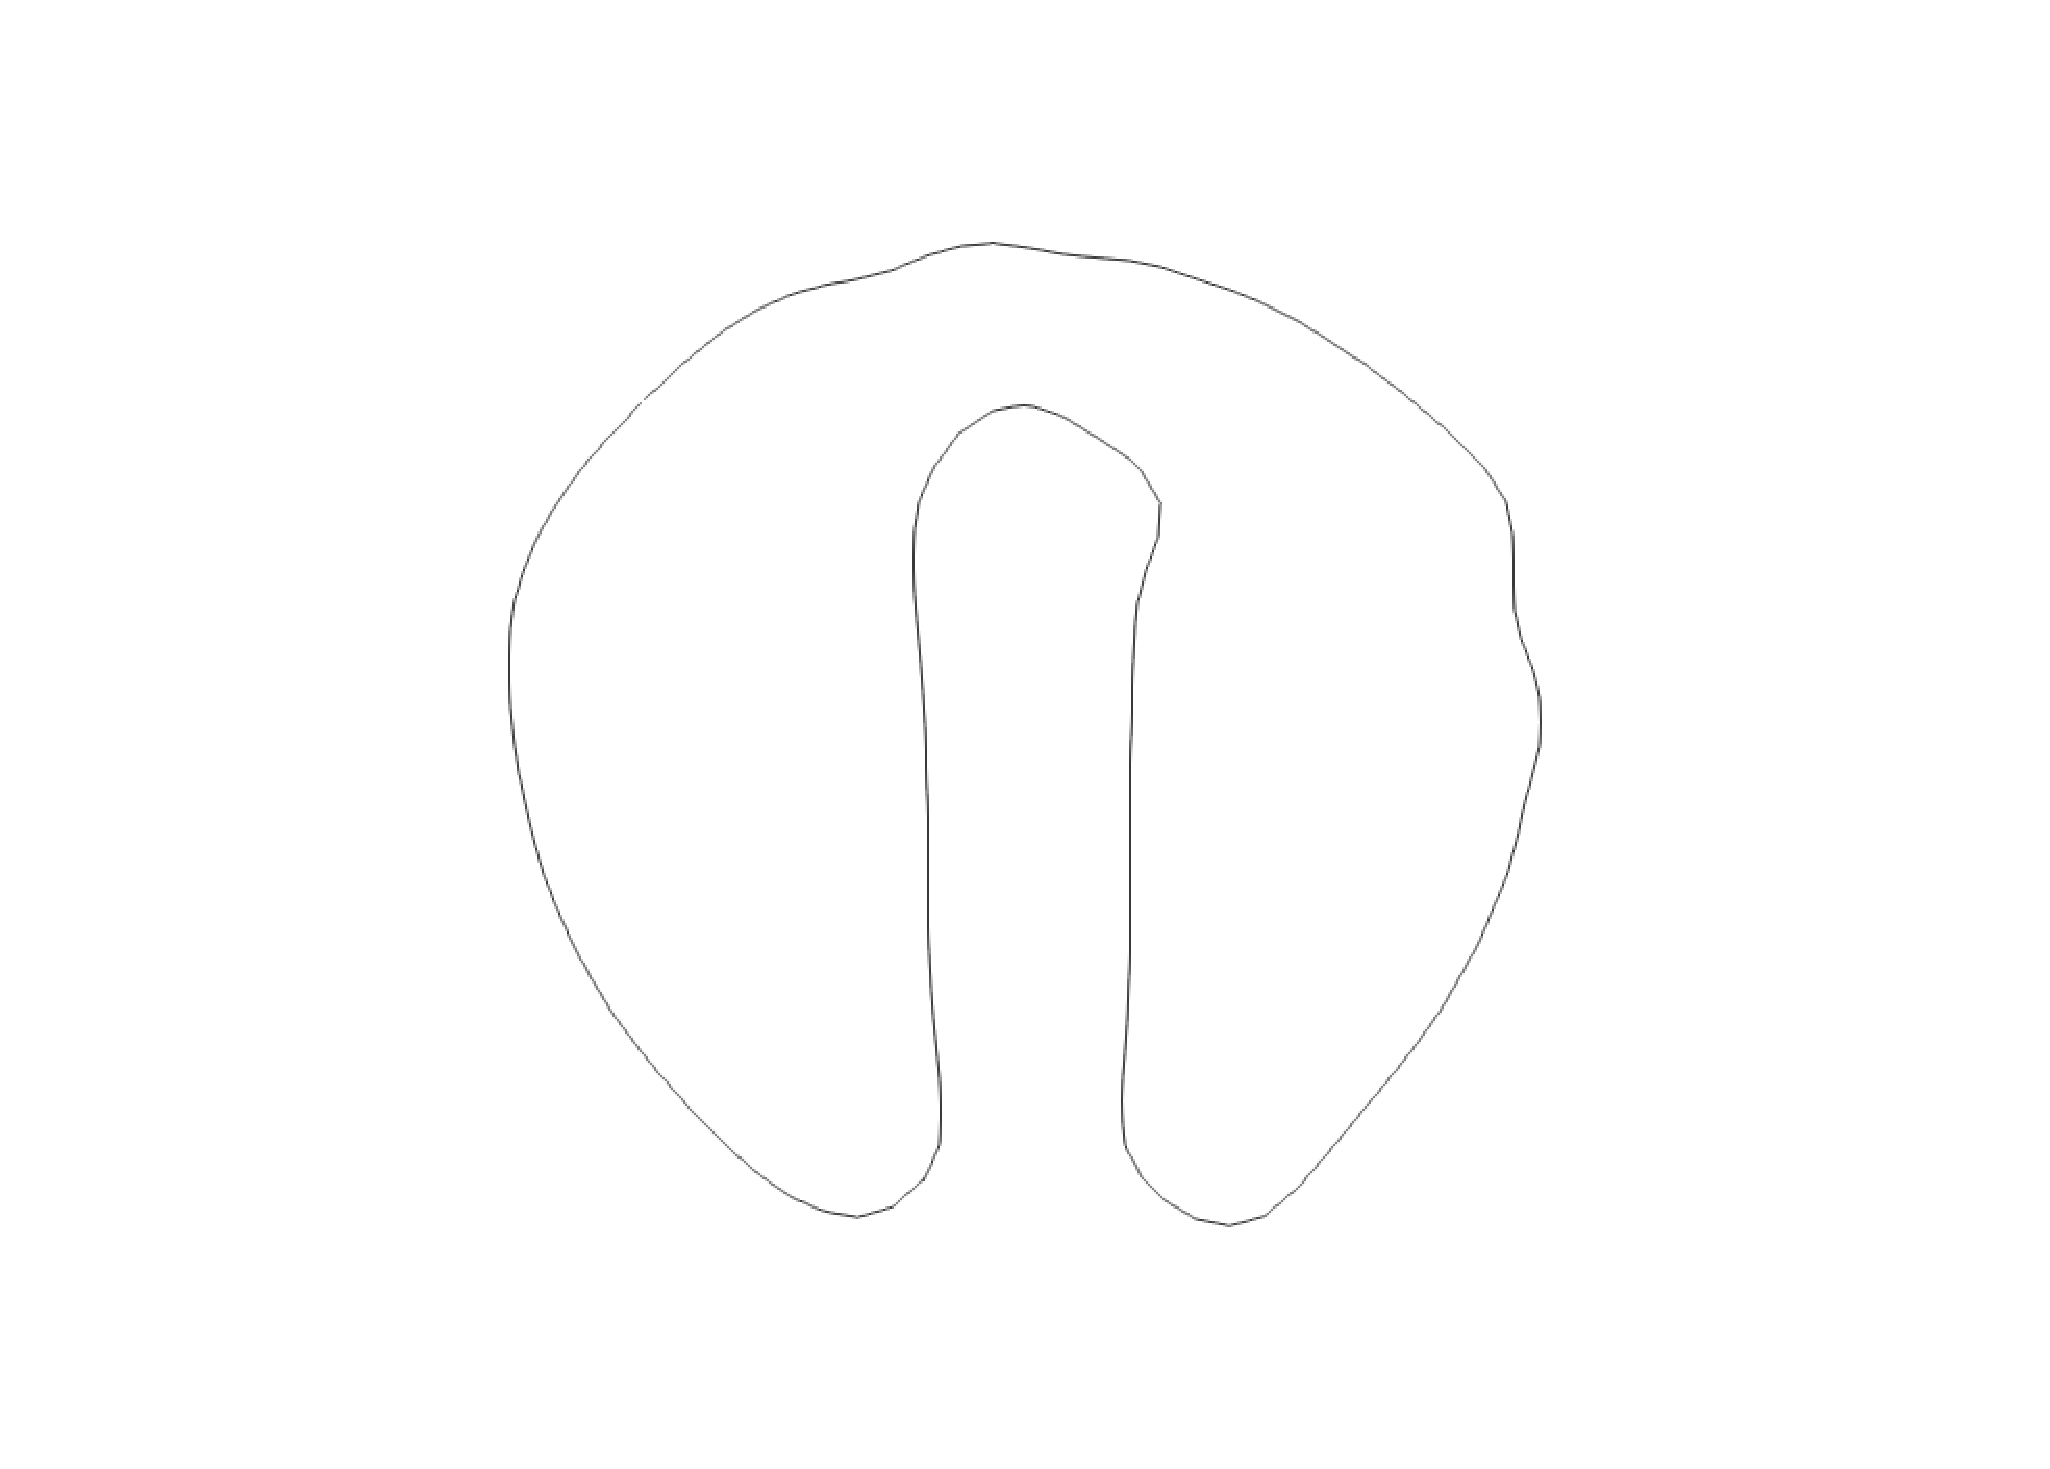
\includegraphics[width=0.3\textwidth]{MULESHexCo01coarse.eps}
%\caption{fig1}
\label{fig:MULESHexCo01coarse}
}
\subfigure[]{
\centering
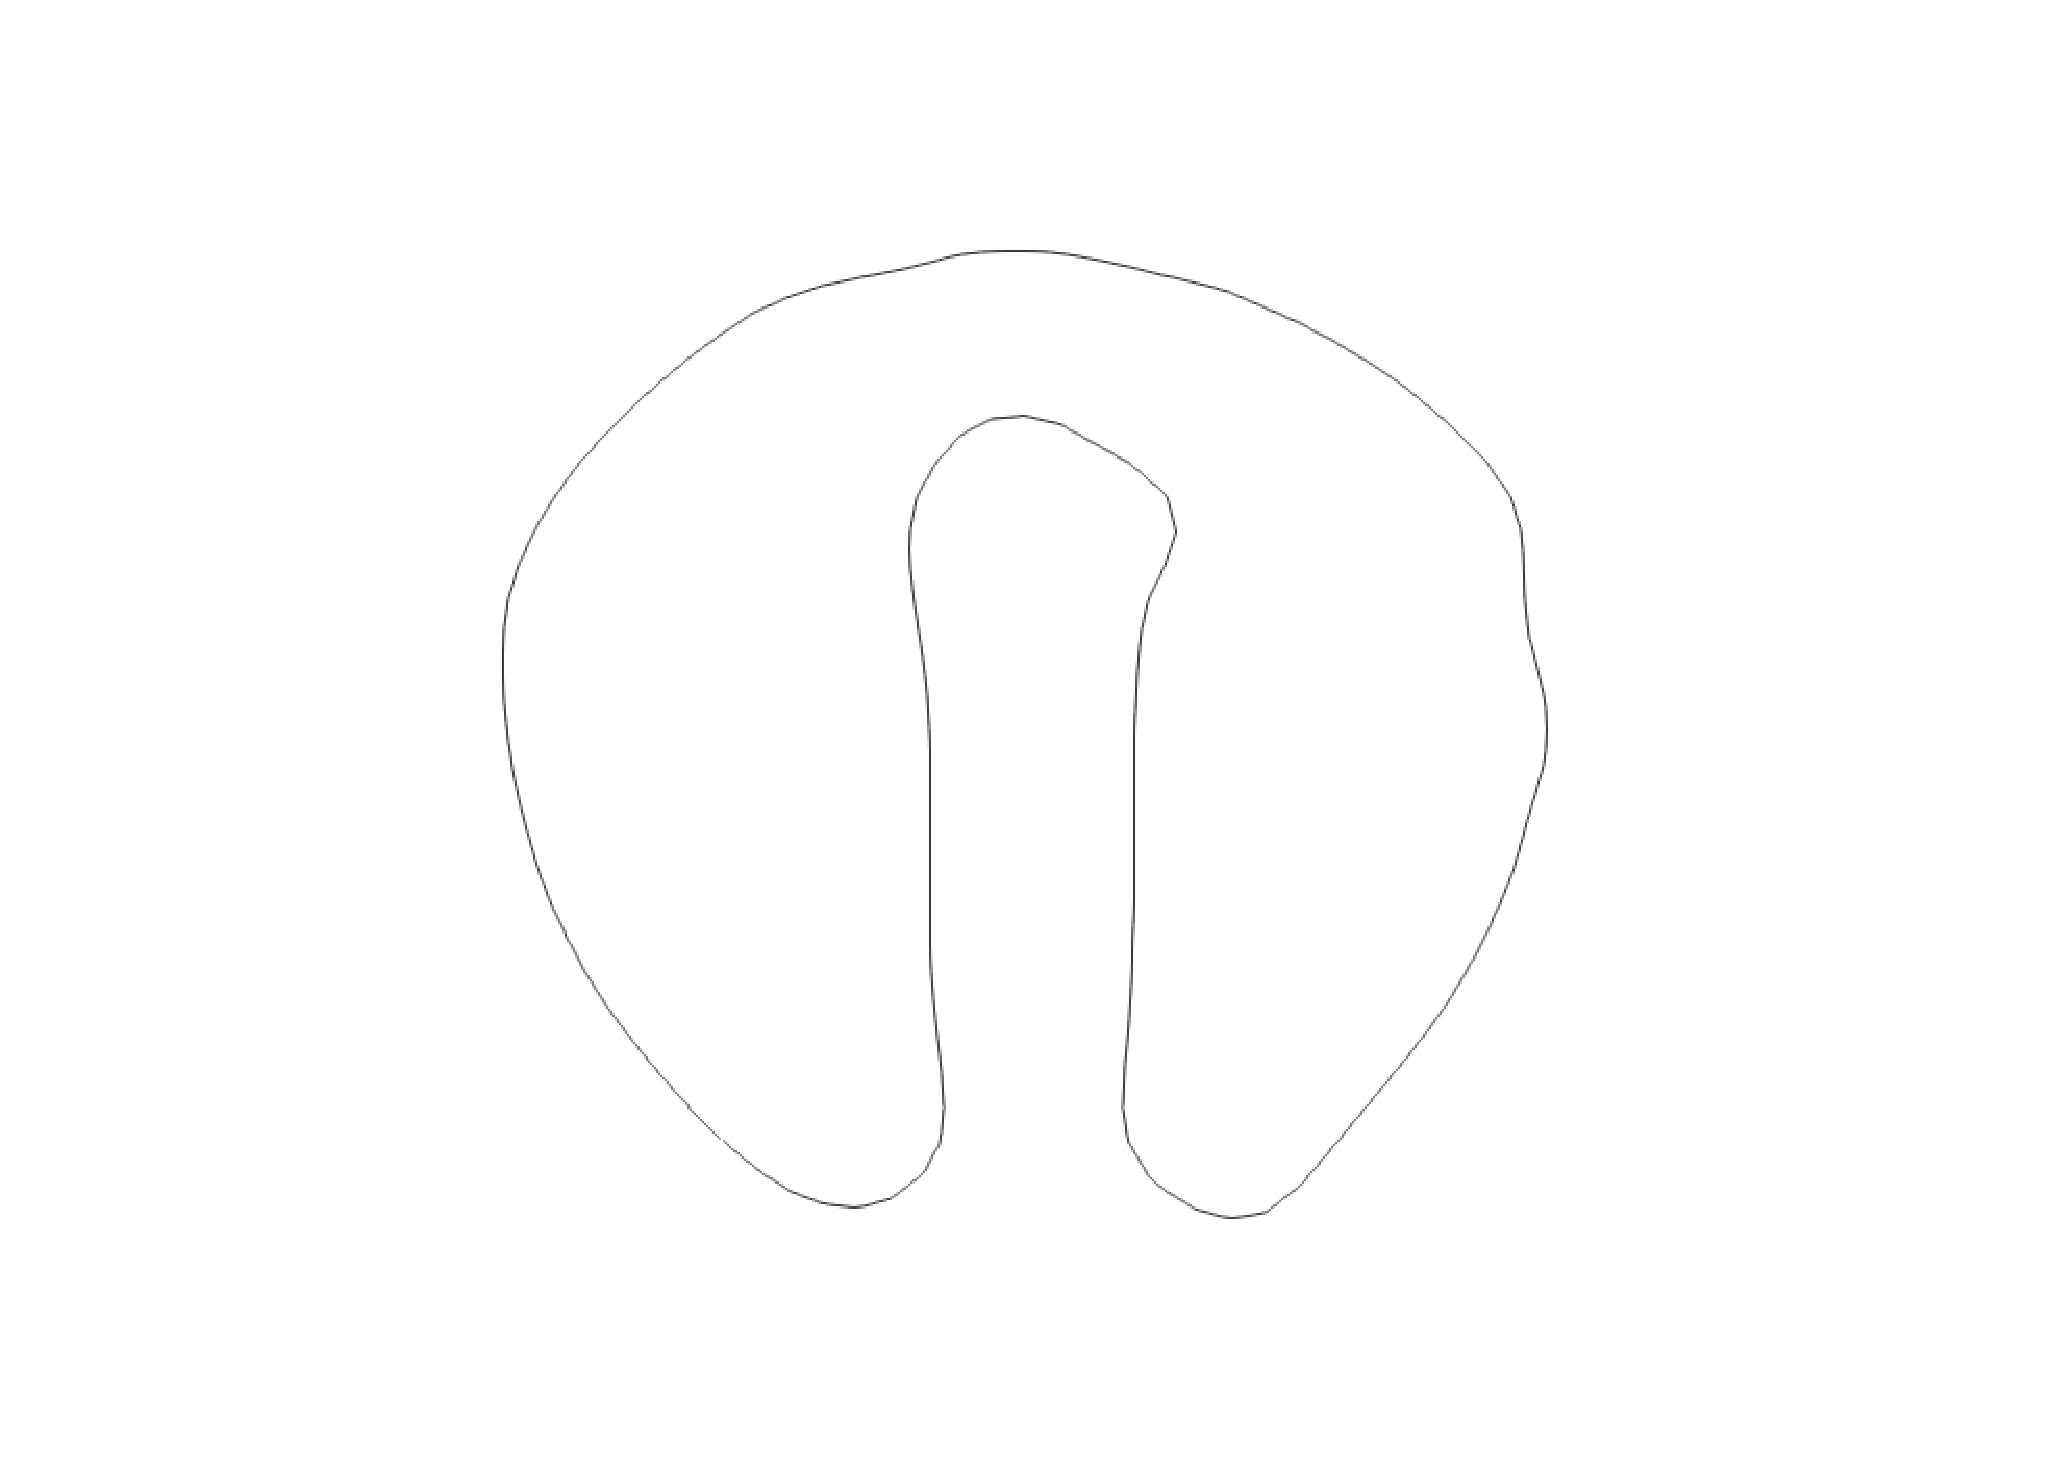
\includegraphics[width=0.3\textwidth]{MULESHexCo02coarse.eps}
\label{fig:MULESHexCo02coarse}
%\caption{fig2}
}
\subfigure[]{
\centering
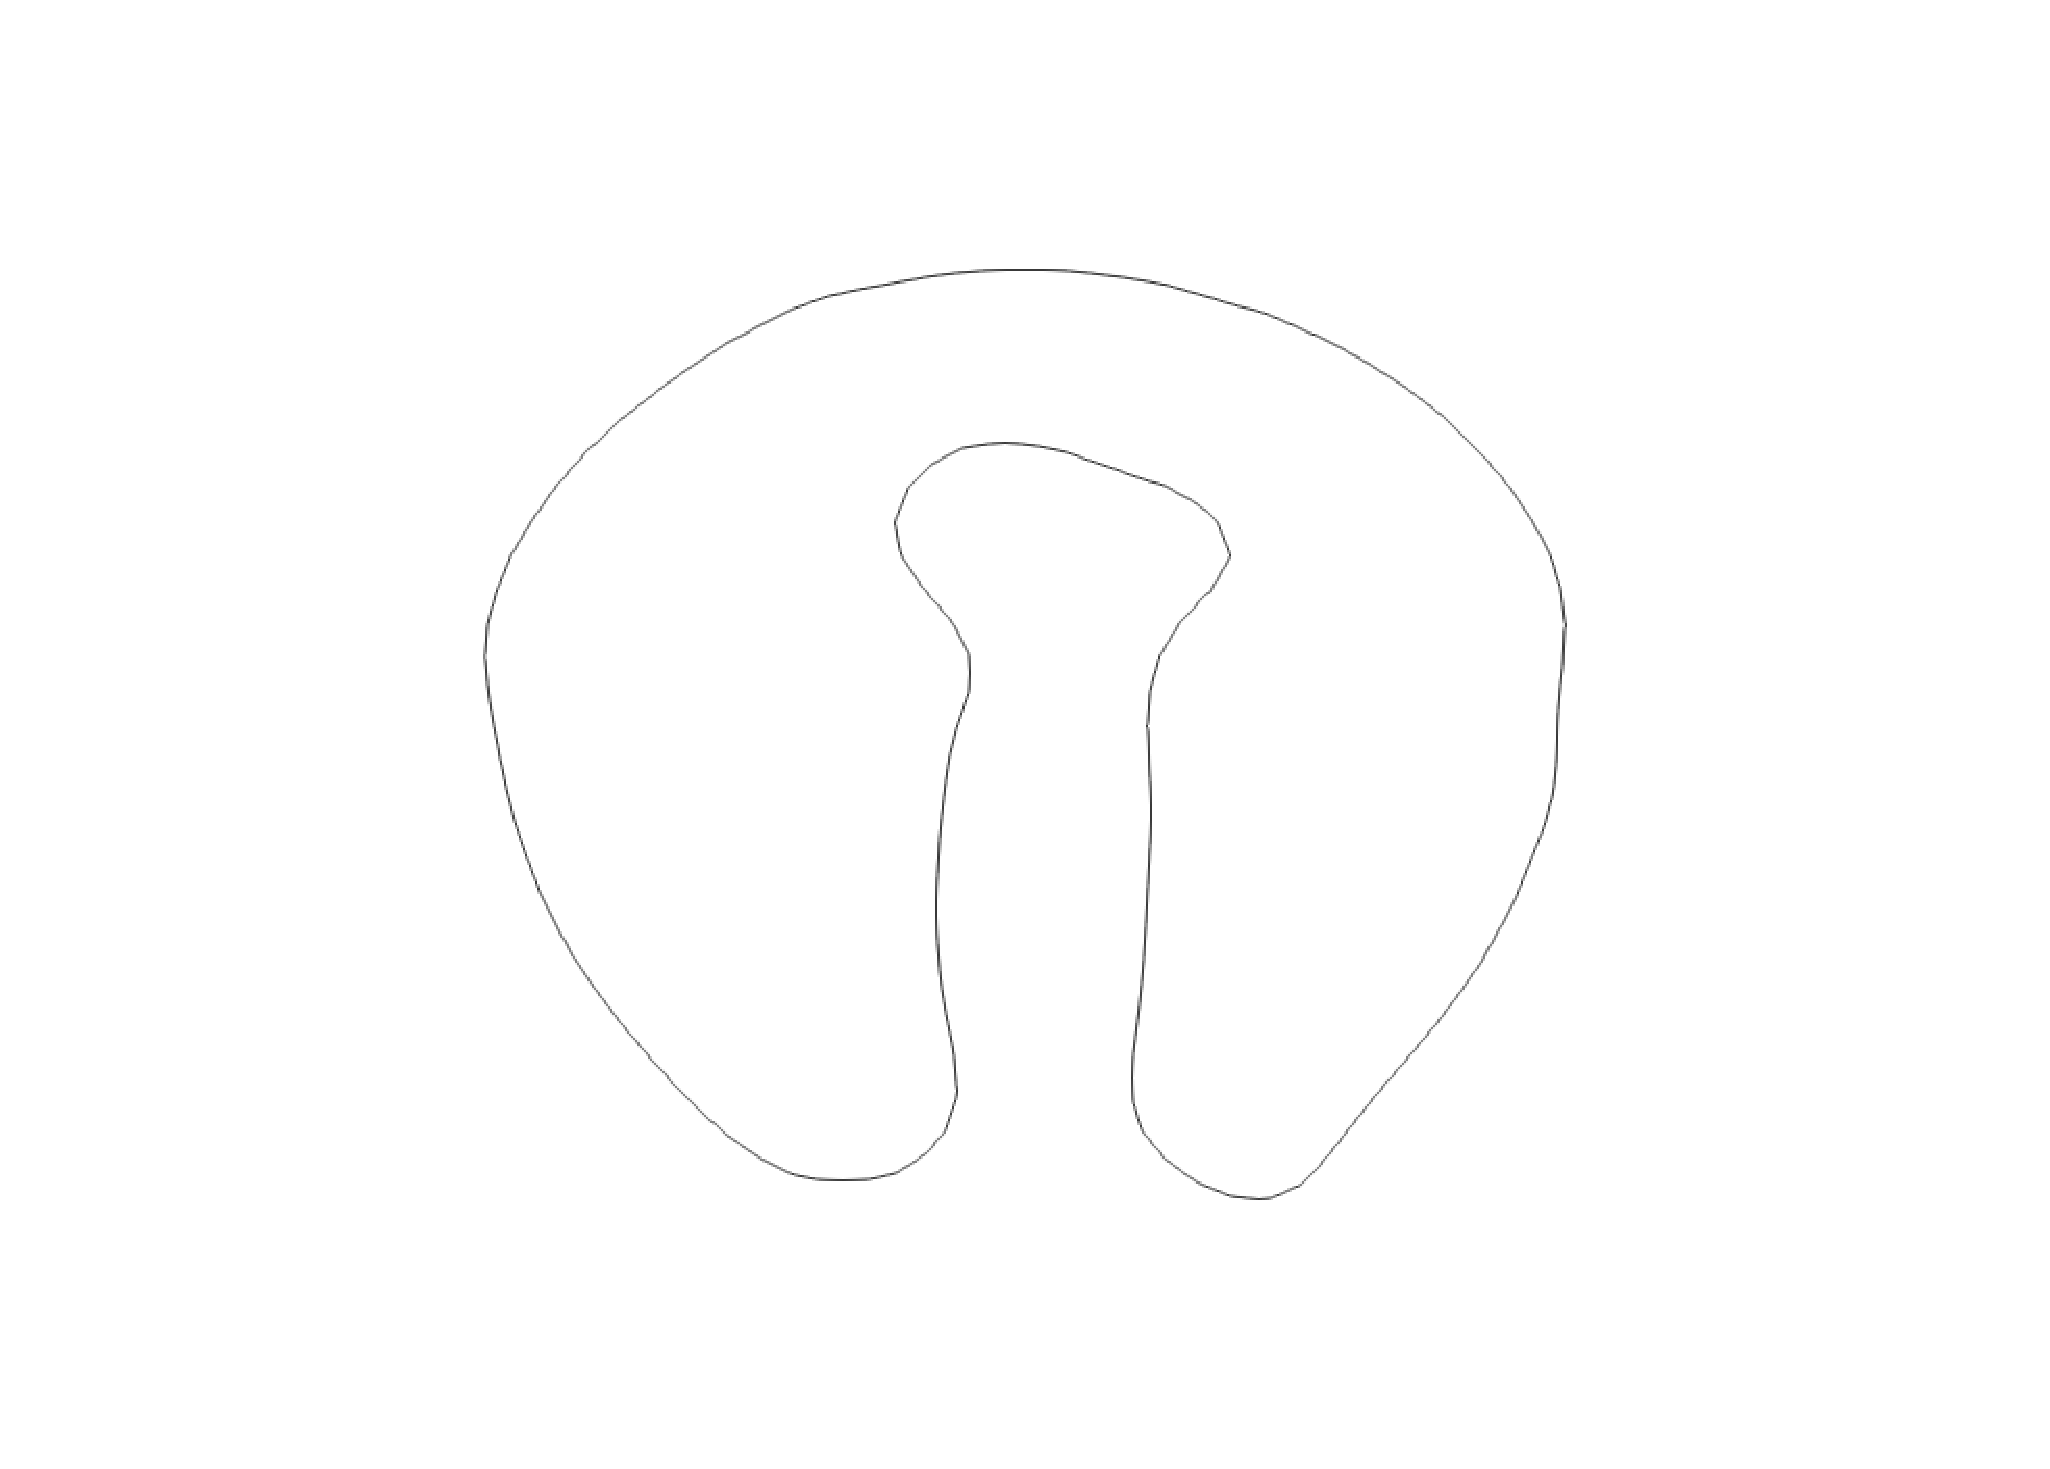
\includegraphics[width=0.3\textwidth]{MULESHexCo05coarse.eps}
\label{fig:MULESHexCo05coarse}
}
\subfigure[]{
\centering
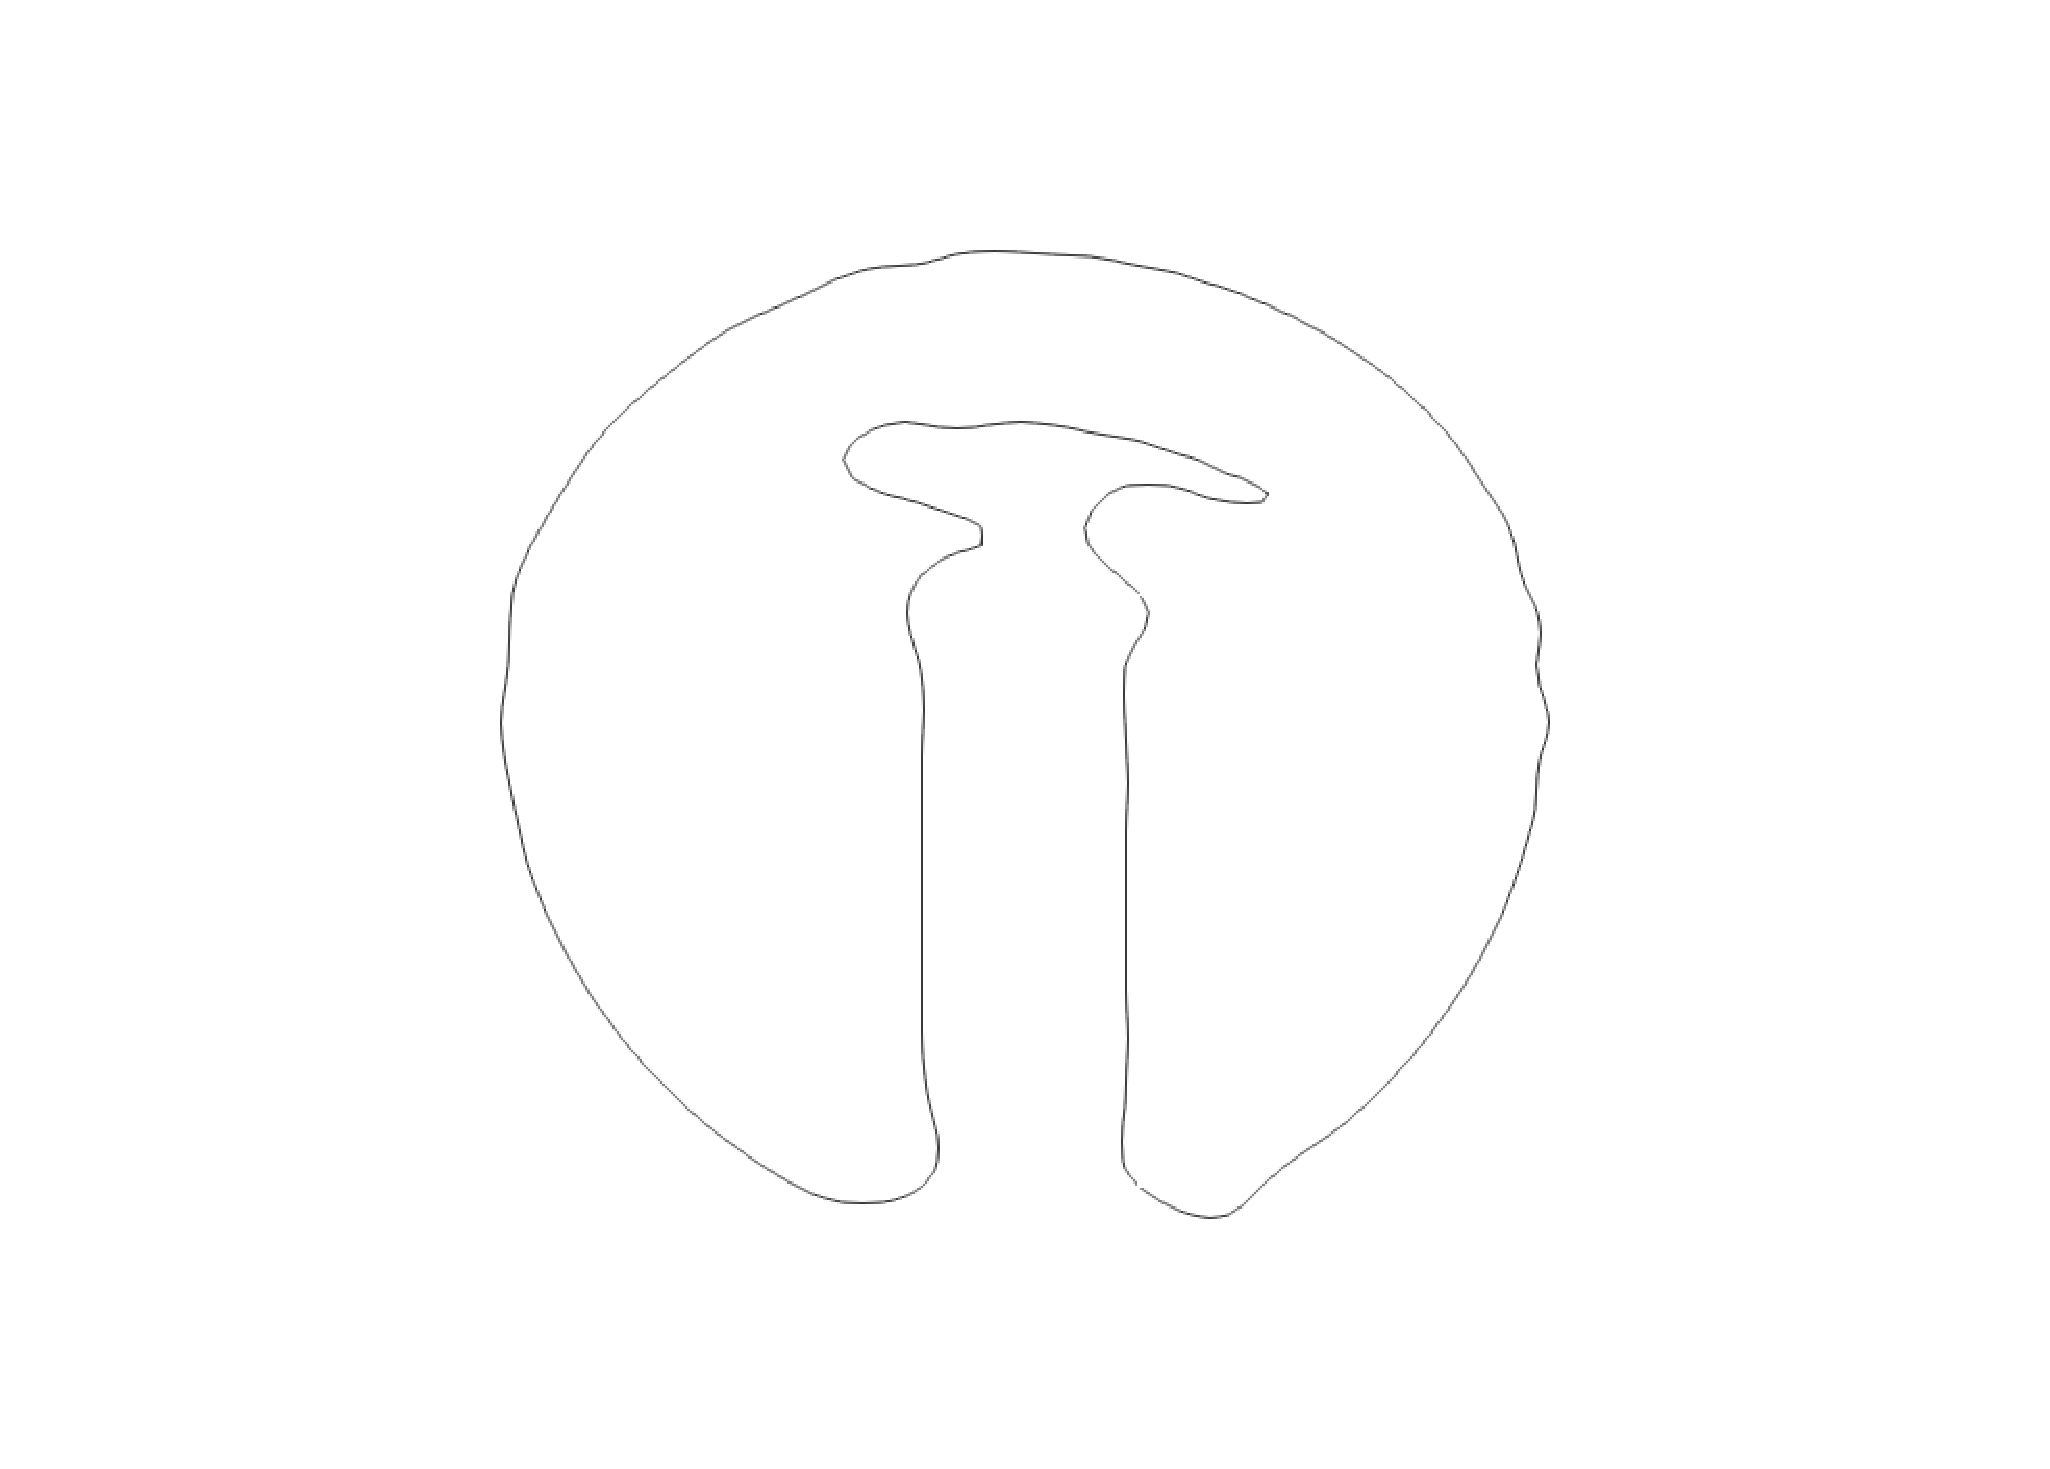
\includegraphics[width=0.3\textwidth]{MULESHexCo05mid.eps}
\label{fig:MULESHexCo05mid}
}
\subfigure[]{
\centering
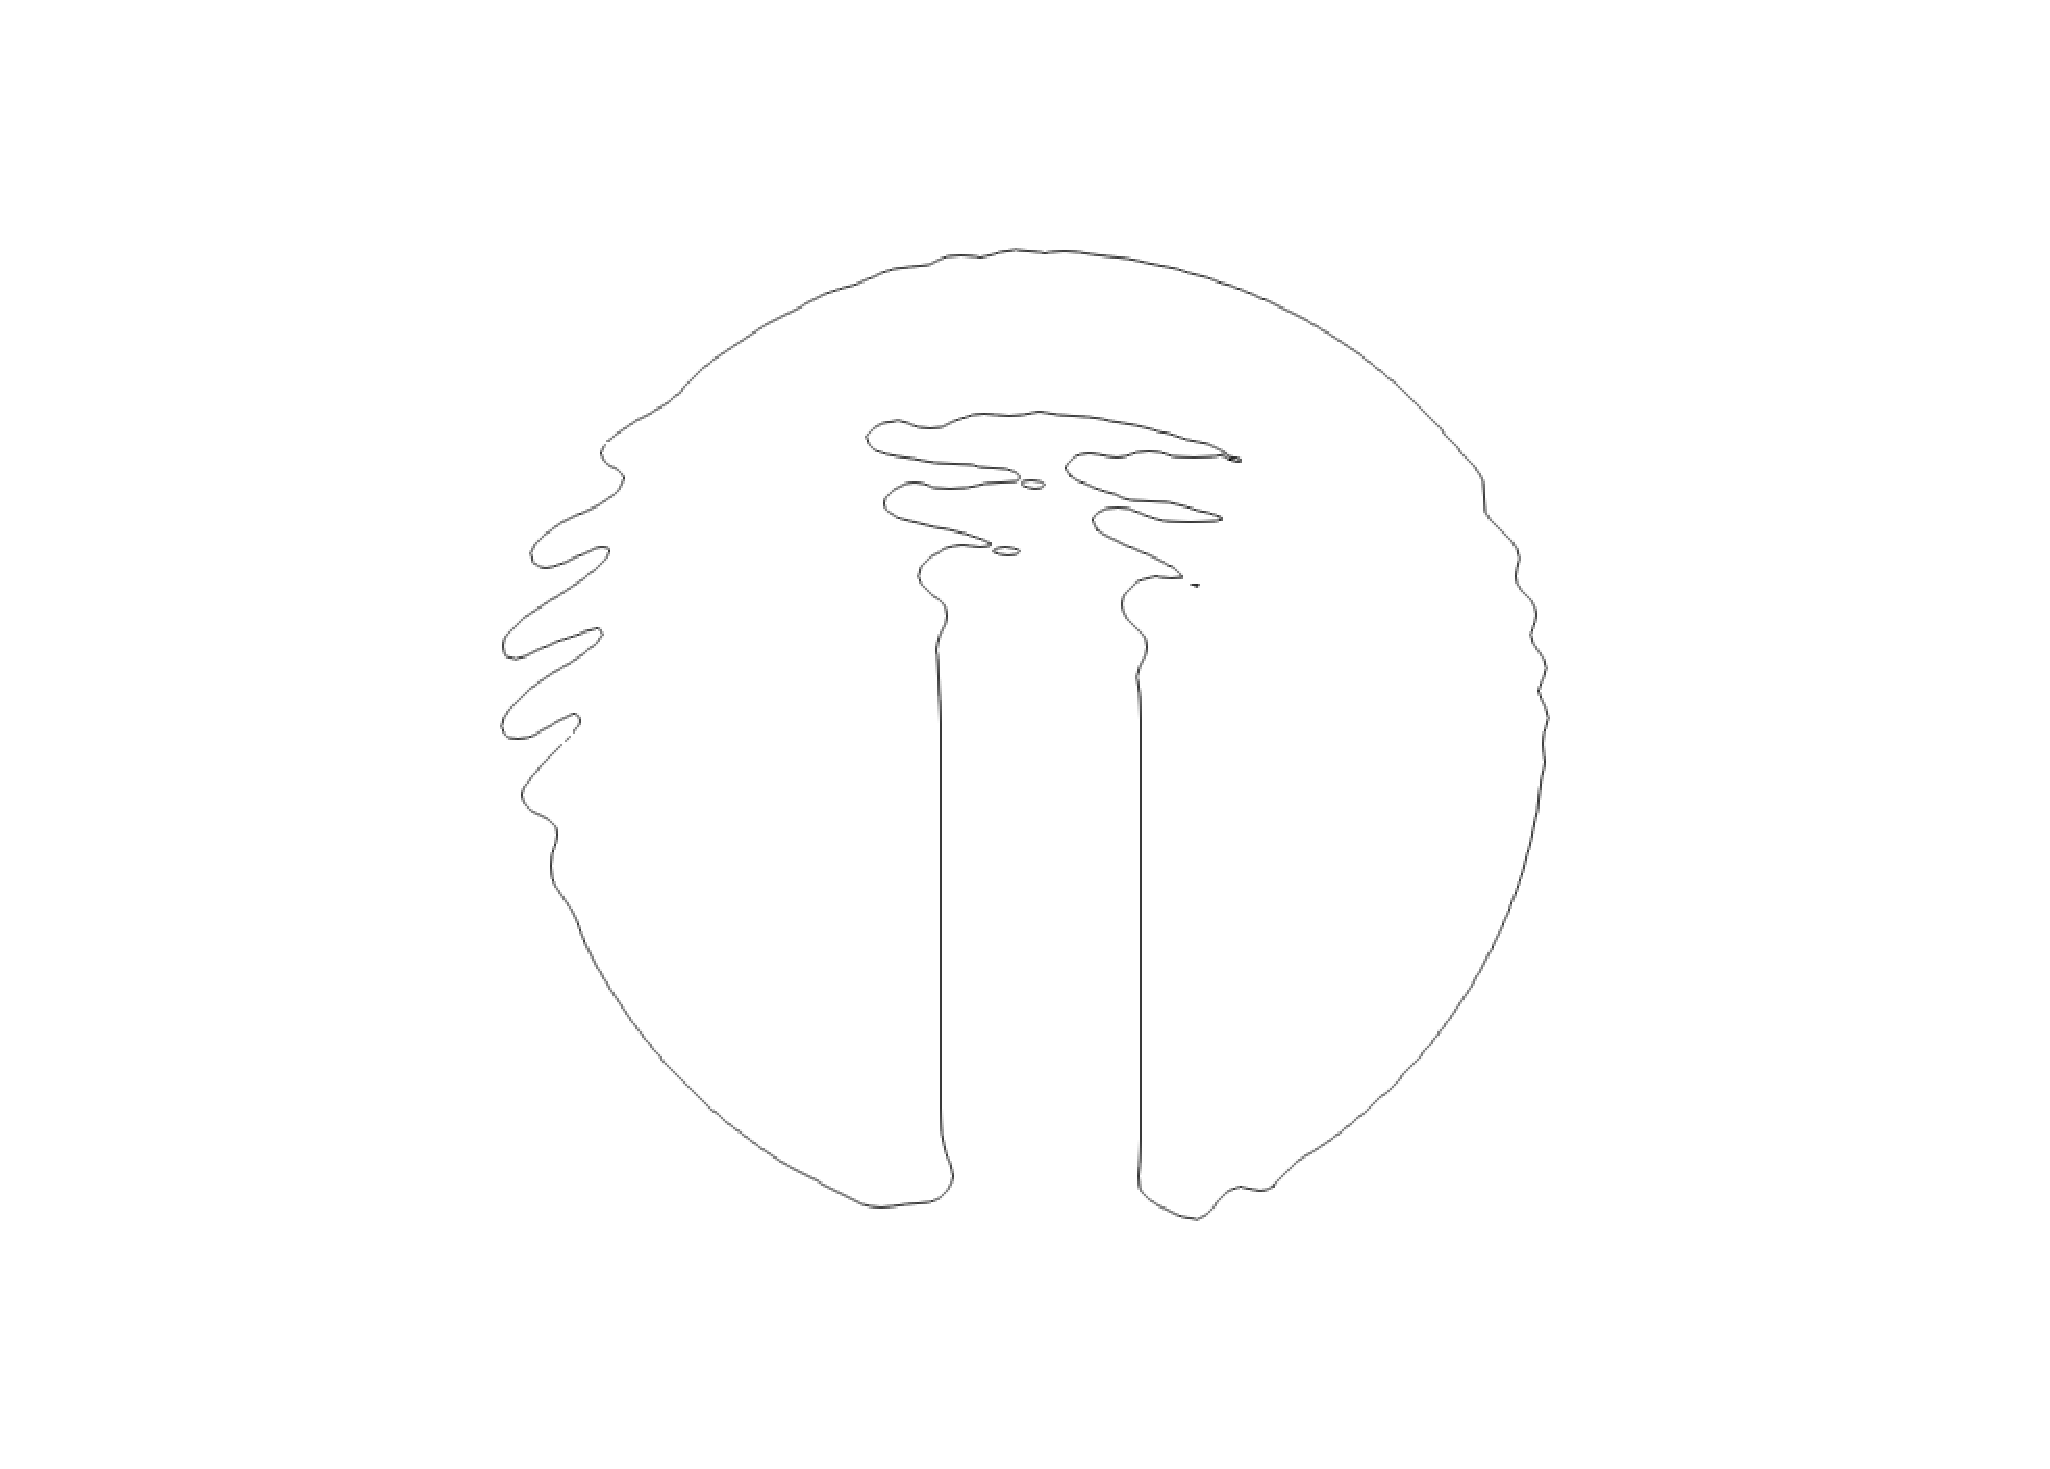
\includegraphics[width=0.3\textwidth]{MULESHexCo05fine.eps}
\label{fig:MULESHexCo05fine}
}
\caption{The shape after one circle with MULES method:\subref{fig:MULESHexCo01coarse} $100\times{100}$ and $Co=0.1$,\subref{fig:MULESHexCo02coarse} $100\times{100}$ and $Co=0.2$,\subref{fig:MULESHexCo05coarse} $100\times{100}$ and $Co=0.5$,\subref{fig:MULESHexCo05mid} $200\times{200}$ and $Co=0.5$,\subref{fig:MULESHexCo05fine} $400\times{400}$ and $Co=0.5$,}
\label{fig:MULESHEX}
\end{figure}
%%%%%%%%%%%%%%%%%%%%%%%%%%%%%%%%%%%%%%%%%%%%%%%%
\begin{figure}[htbp]
\centering
\subfigure[]{
\centering
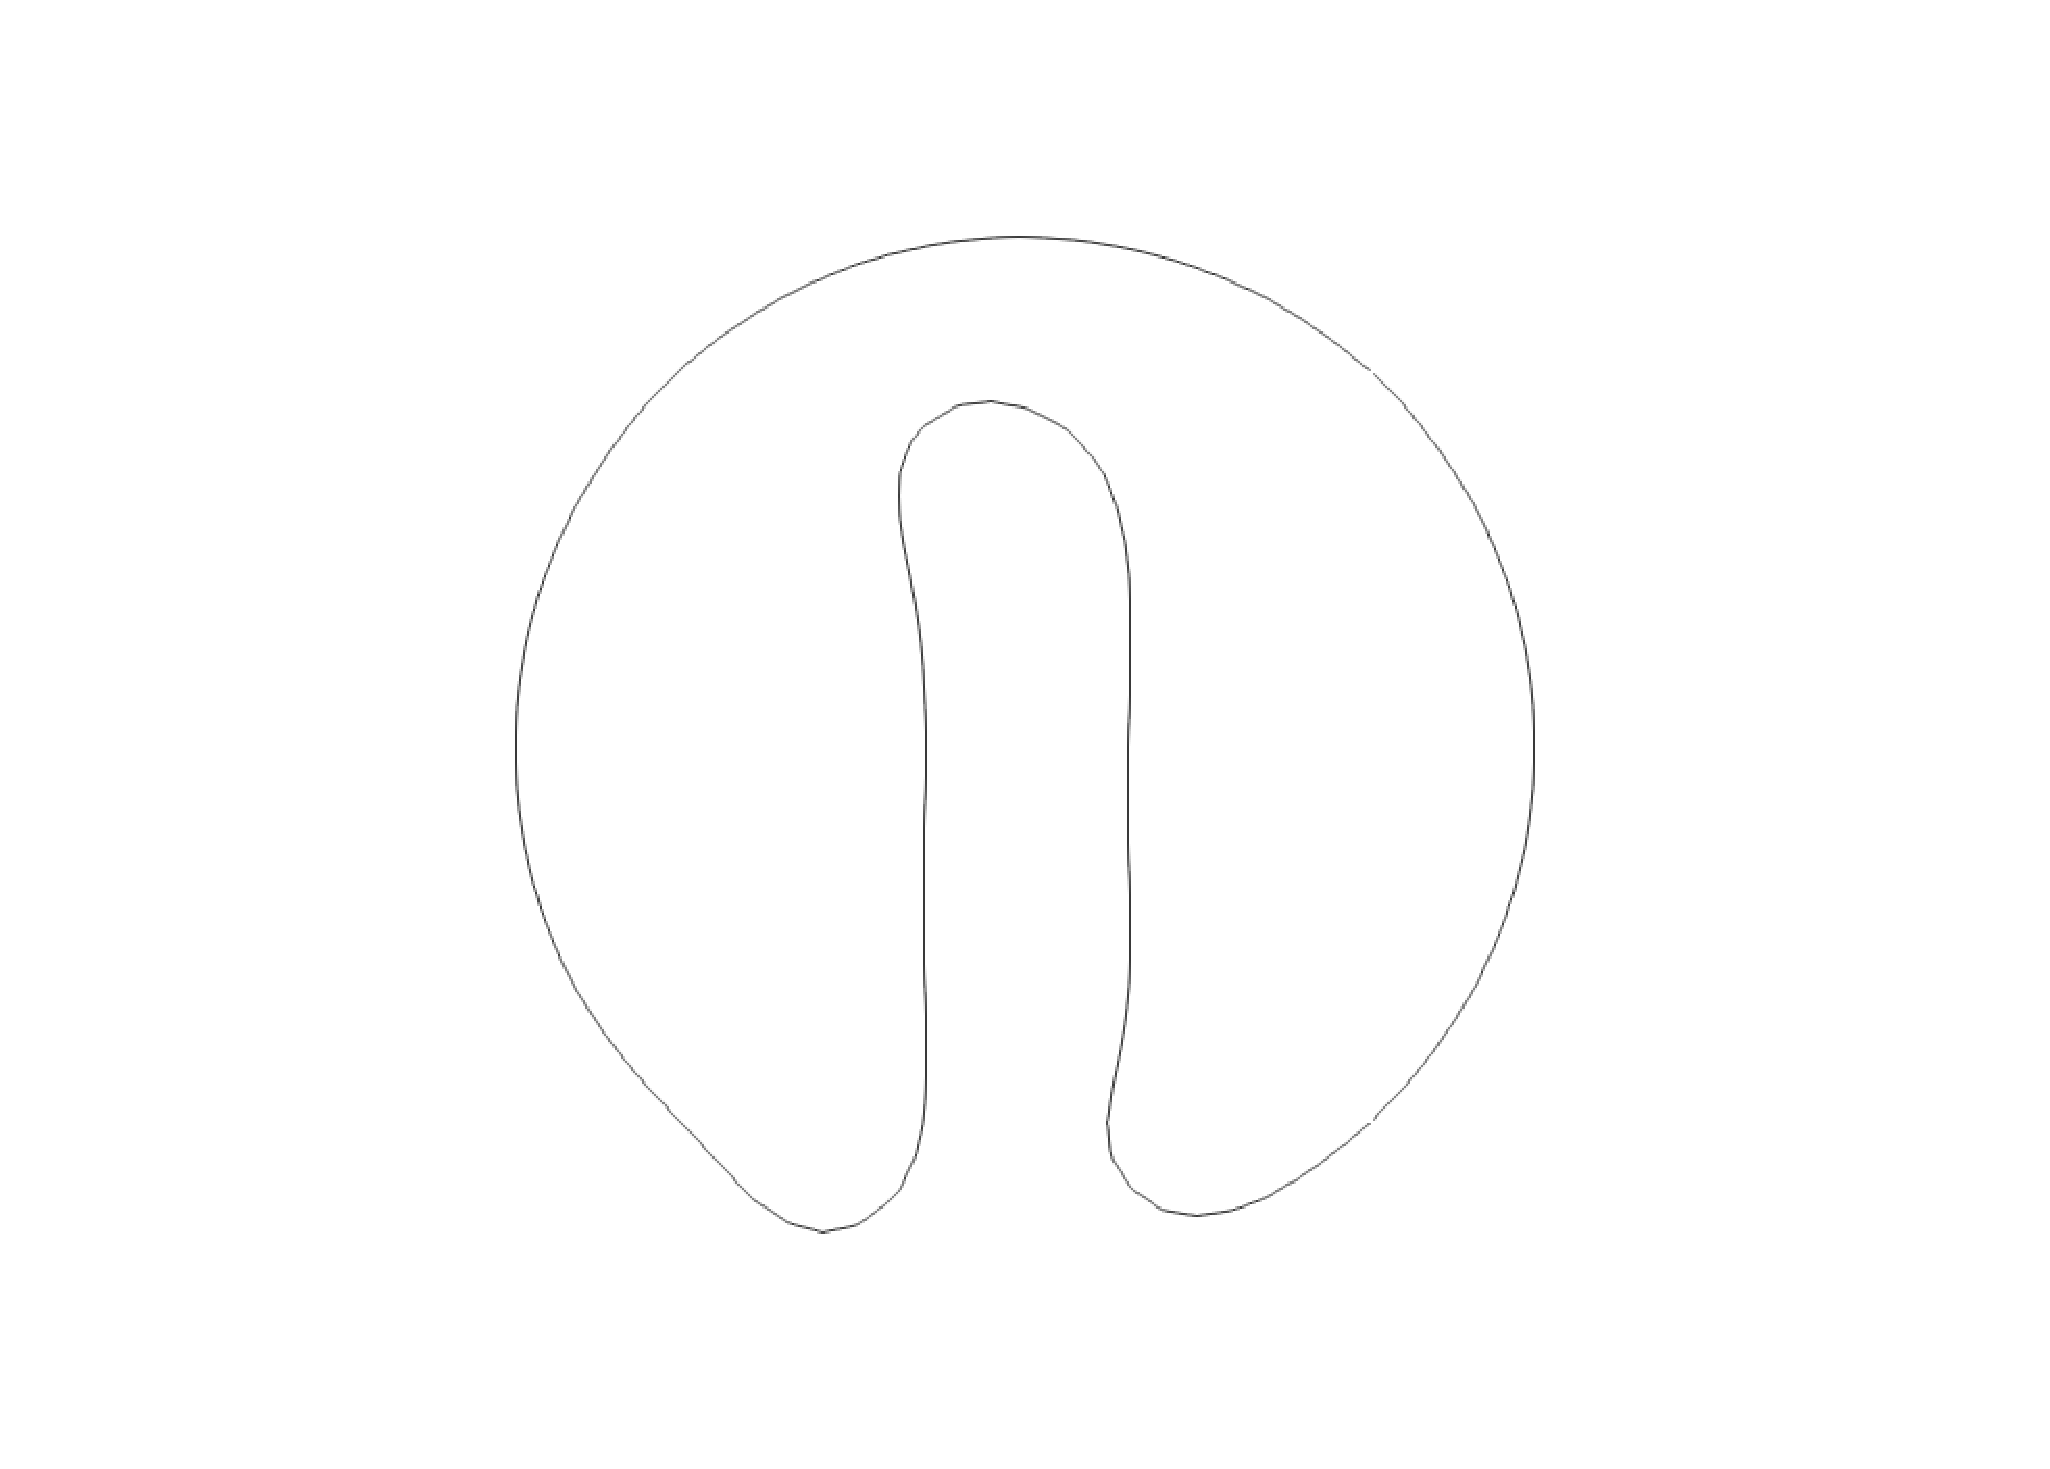
\includegraphics[width=0.3\textwidth]{isoHexCo01coarse.eps}
%\caption{fig1}
\label{fig:ISOHexCo01coarse}
}
\subfigure[]{
\centering
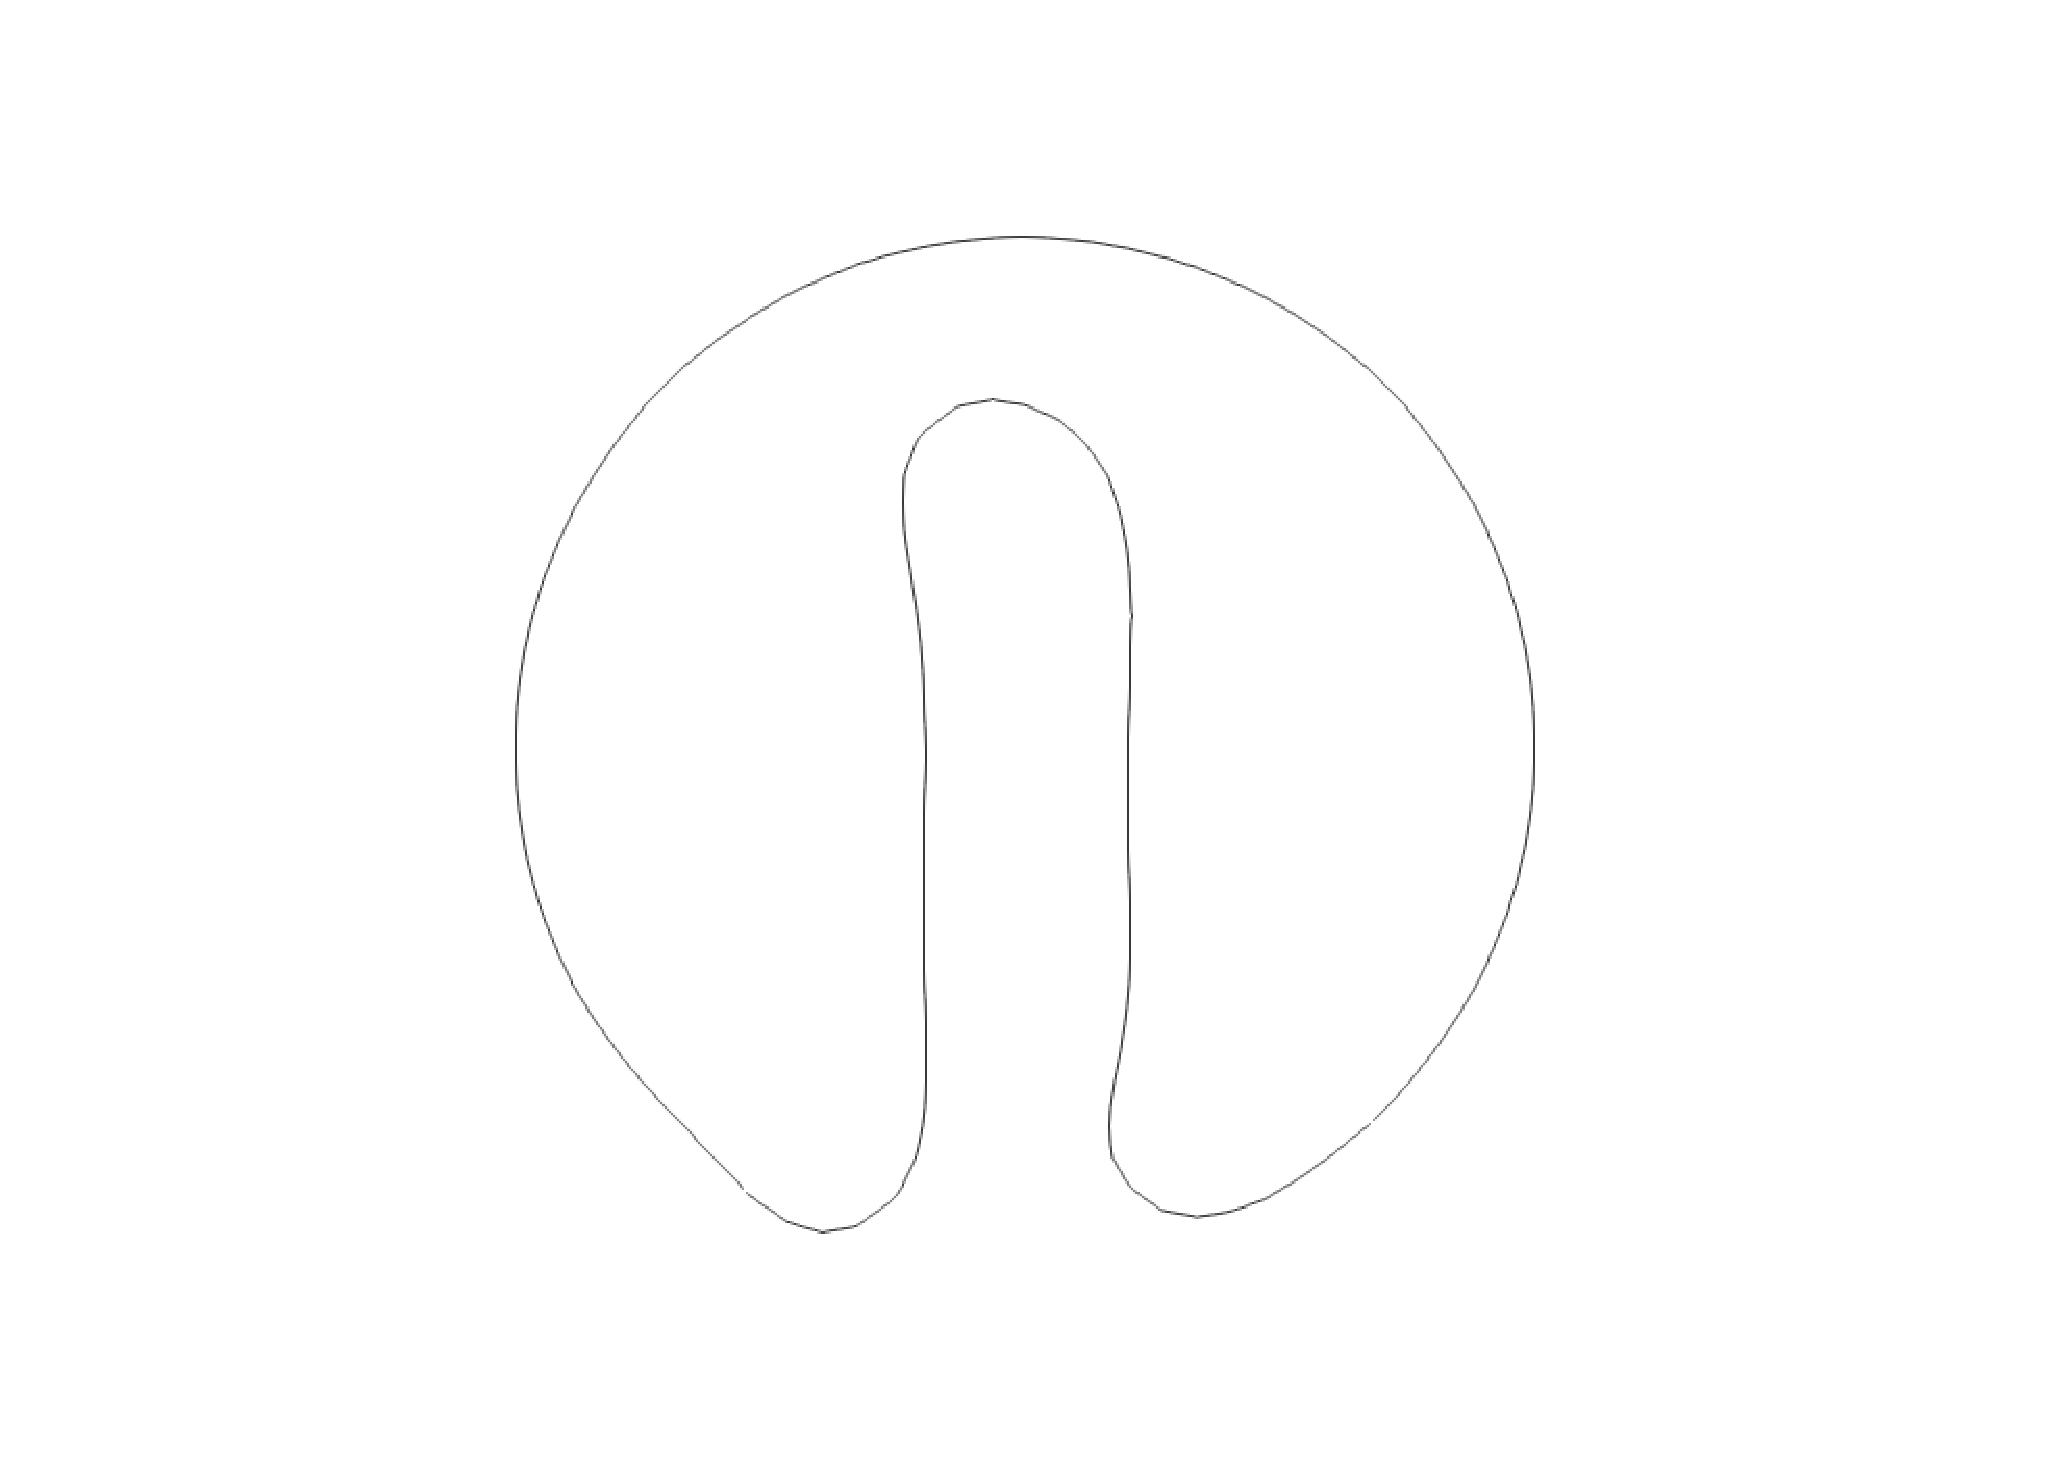
\includegraphics[width=0.3\textwidth]{isoHexCo02coarse.eps}
\label{fig:ISOHexCo02coarse}
%\caption{fig2}
}
\subfigure[]{
\centering
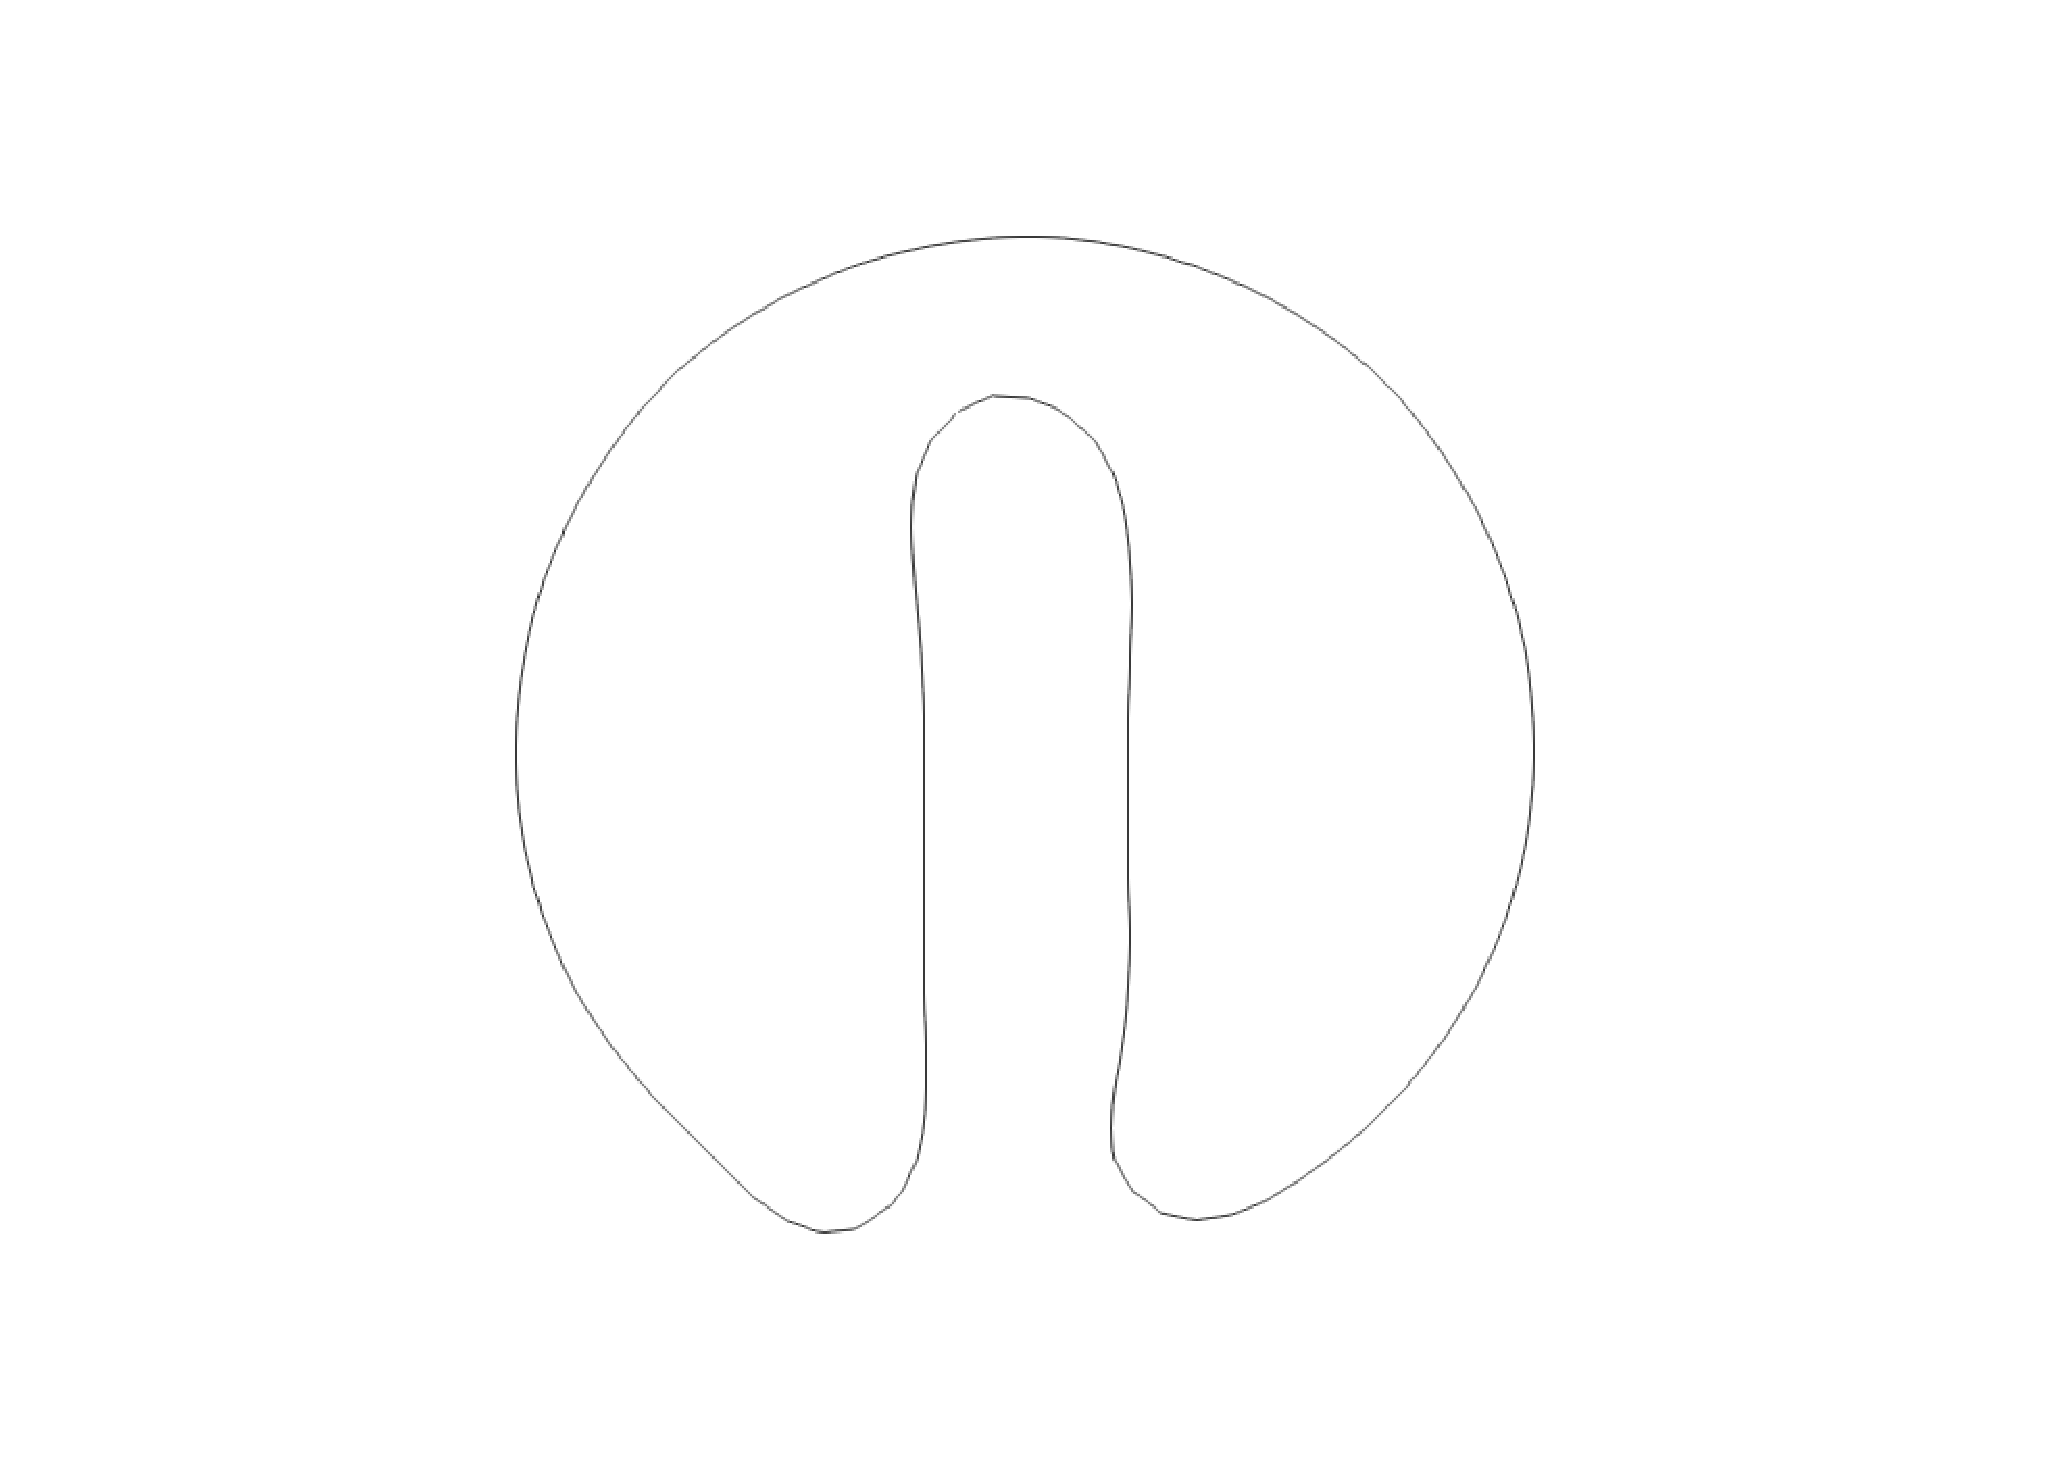
\includegraphics[width=0.3\textwidth]{isoHexCo05coarse.eps}
\label{fig:ISOHexCo05coarse}
}
\subfigure[]{
\centering
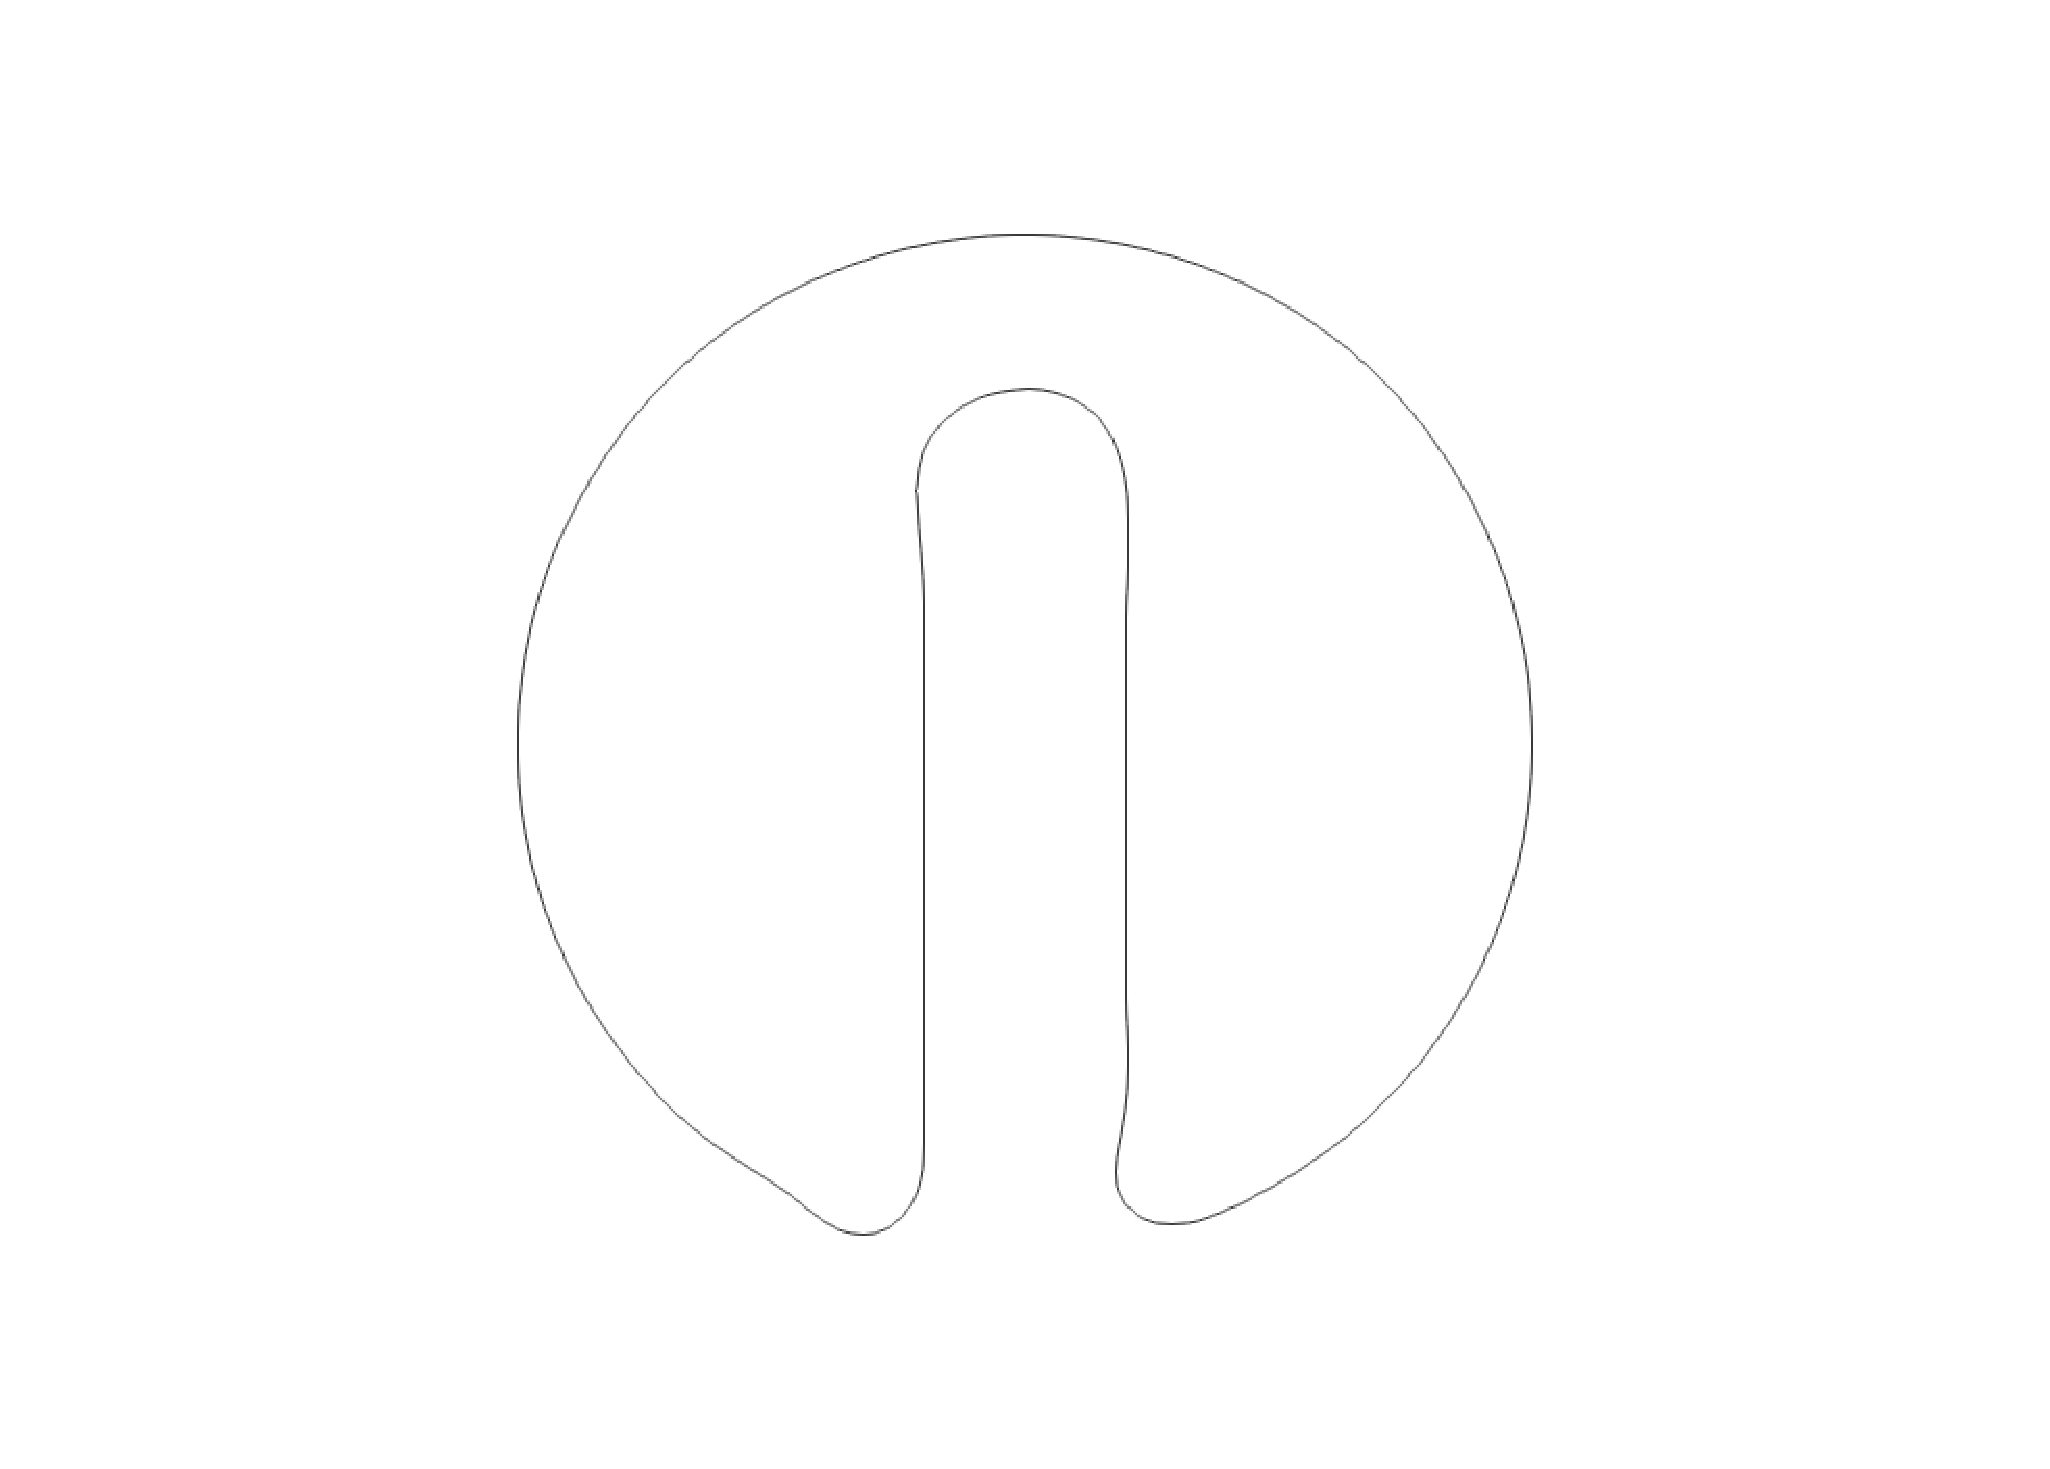
\includegraphics[width=0.3\textwidth]{isoHexCo05mid.eps}
\label{fig:ISOHexCo05mid}
}
\subfigure[]{
\centering
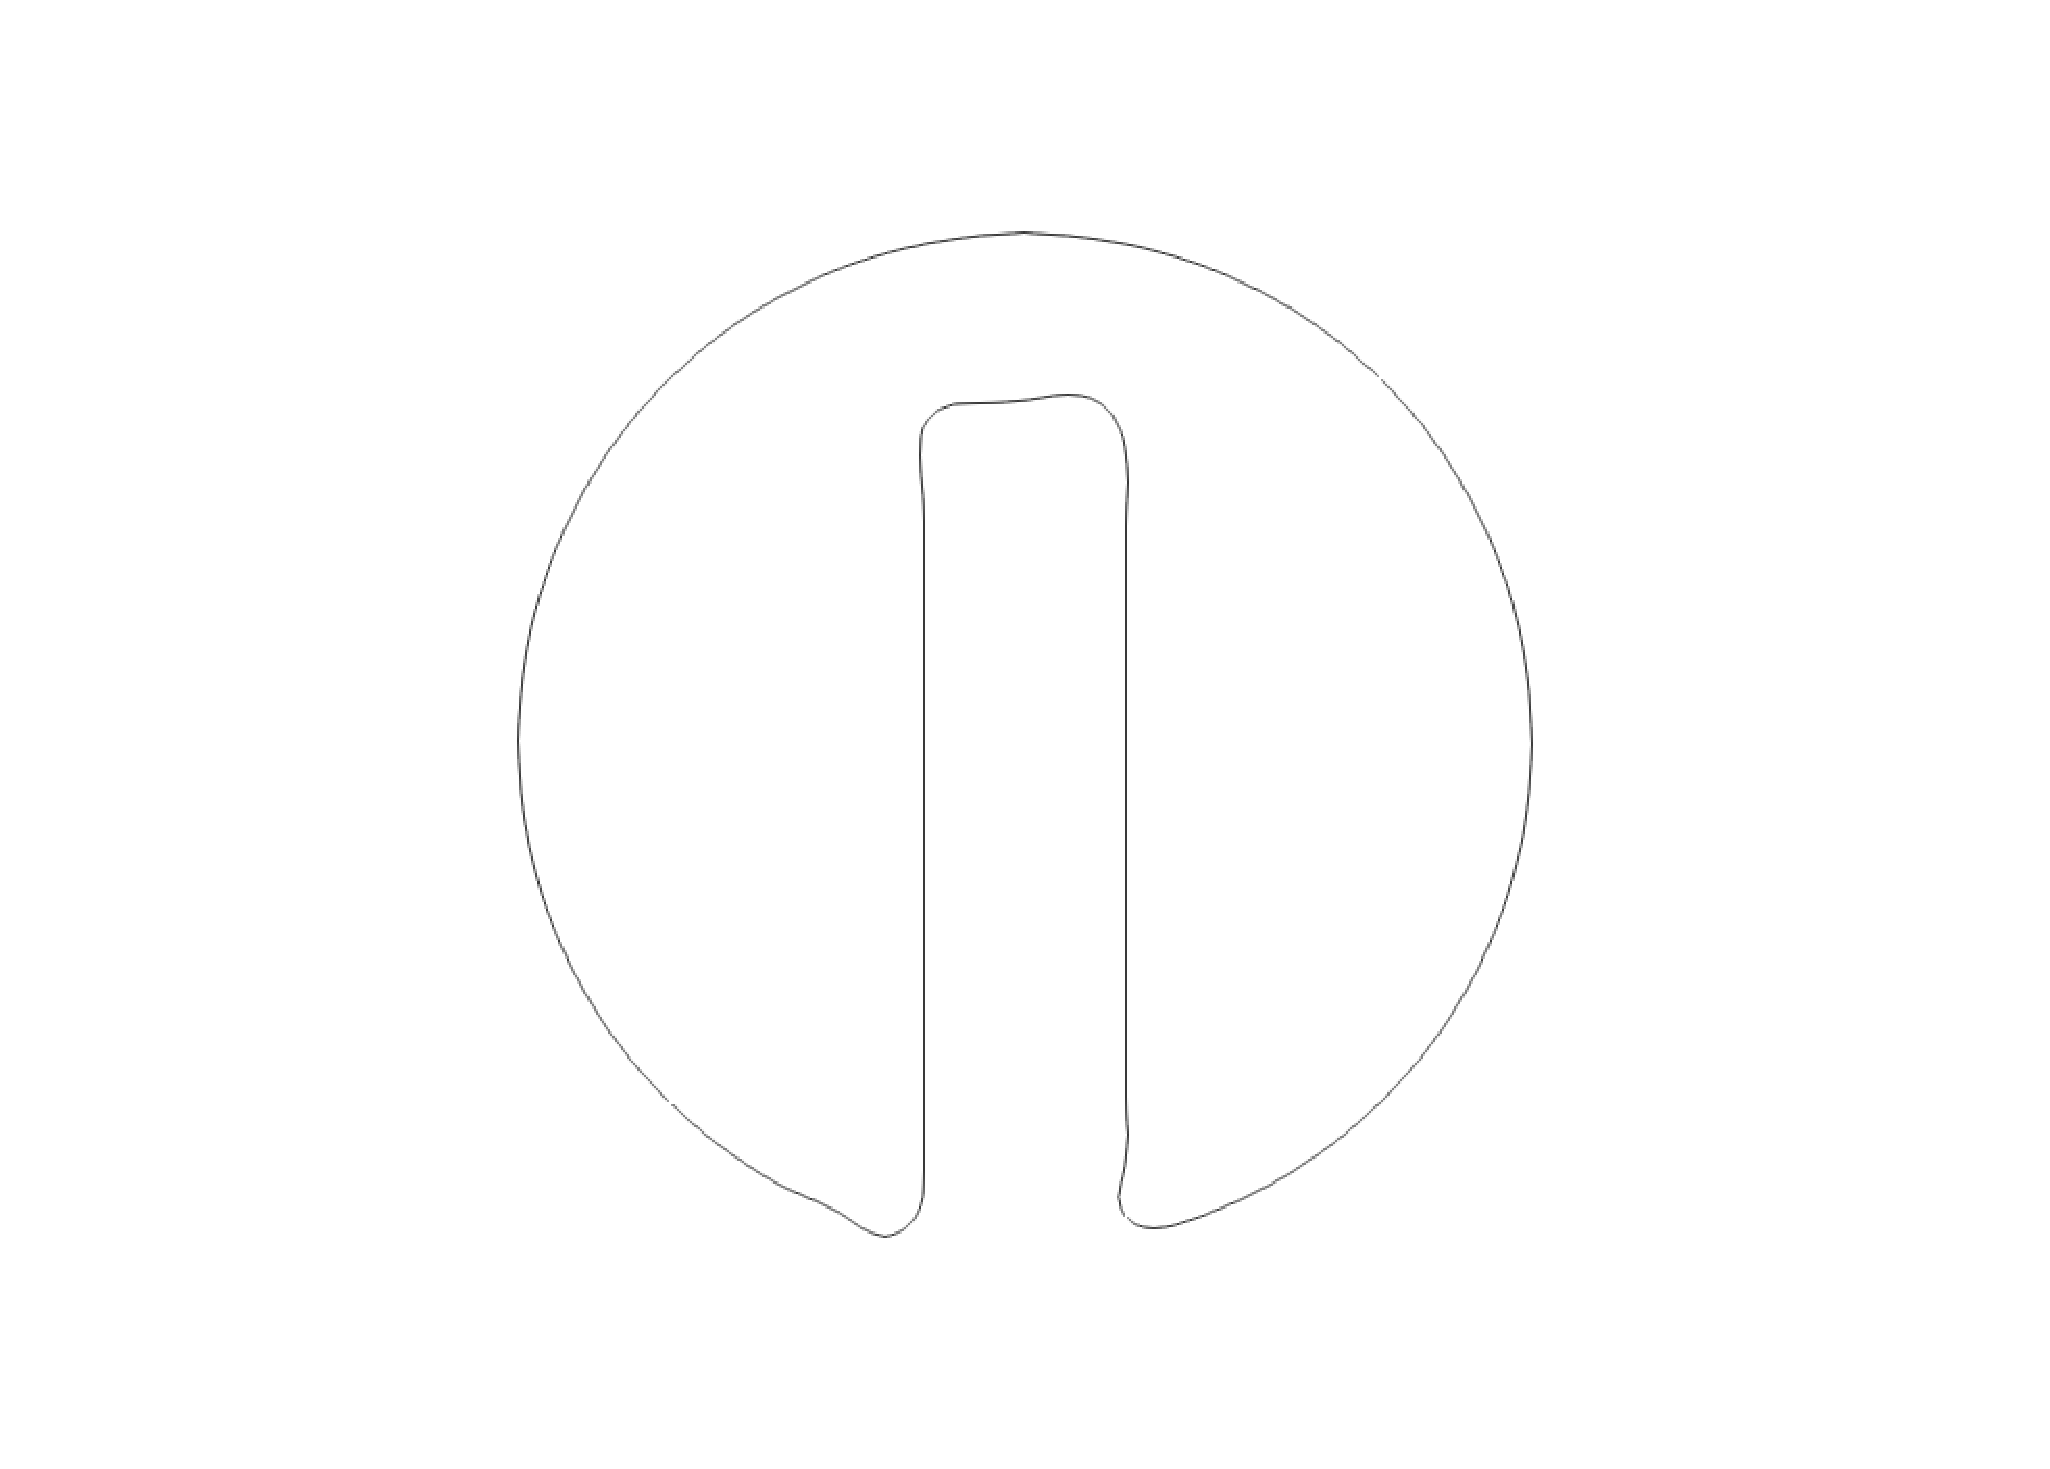
\includegraphics[width=0.3\textwidth]{isoHexCo05fine.eps}
\label{fig:ISOHexCo05fine}
}
\caption{The shape after one circle with isoAdvector method:\subref{fig:ISOHexCo01coarse} $100\times{100}$ and $Co=0.1$,\subref{fig:ISOHexCo02coarse} $100\times{100}$ and $Co=0.2$,\subref{fig:ISOHexCo05coarse} $100\times{100}$ and $Co=0.5$,\subref{fig:ISOHexCo05mid} $200\times{200}$ and $Co=0.5$,\subref{fig:ISOHexCo05fine} $400\times{400}$ and $Co=0.5$,}
\label{fig:ISOHEX}
\end{figure}
%%%%%%%%%%%%%%%%%%%%%%%%%%%%%%%%%%%%%%%%%%%%%%%%%%%%%%%%%%
\begin{figure}[htbp]
\centering
\subfigure[]{
\centering
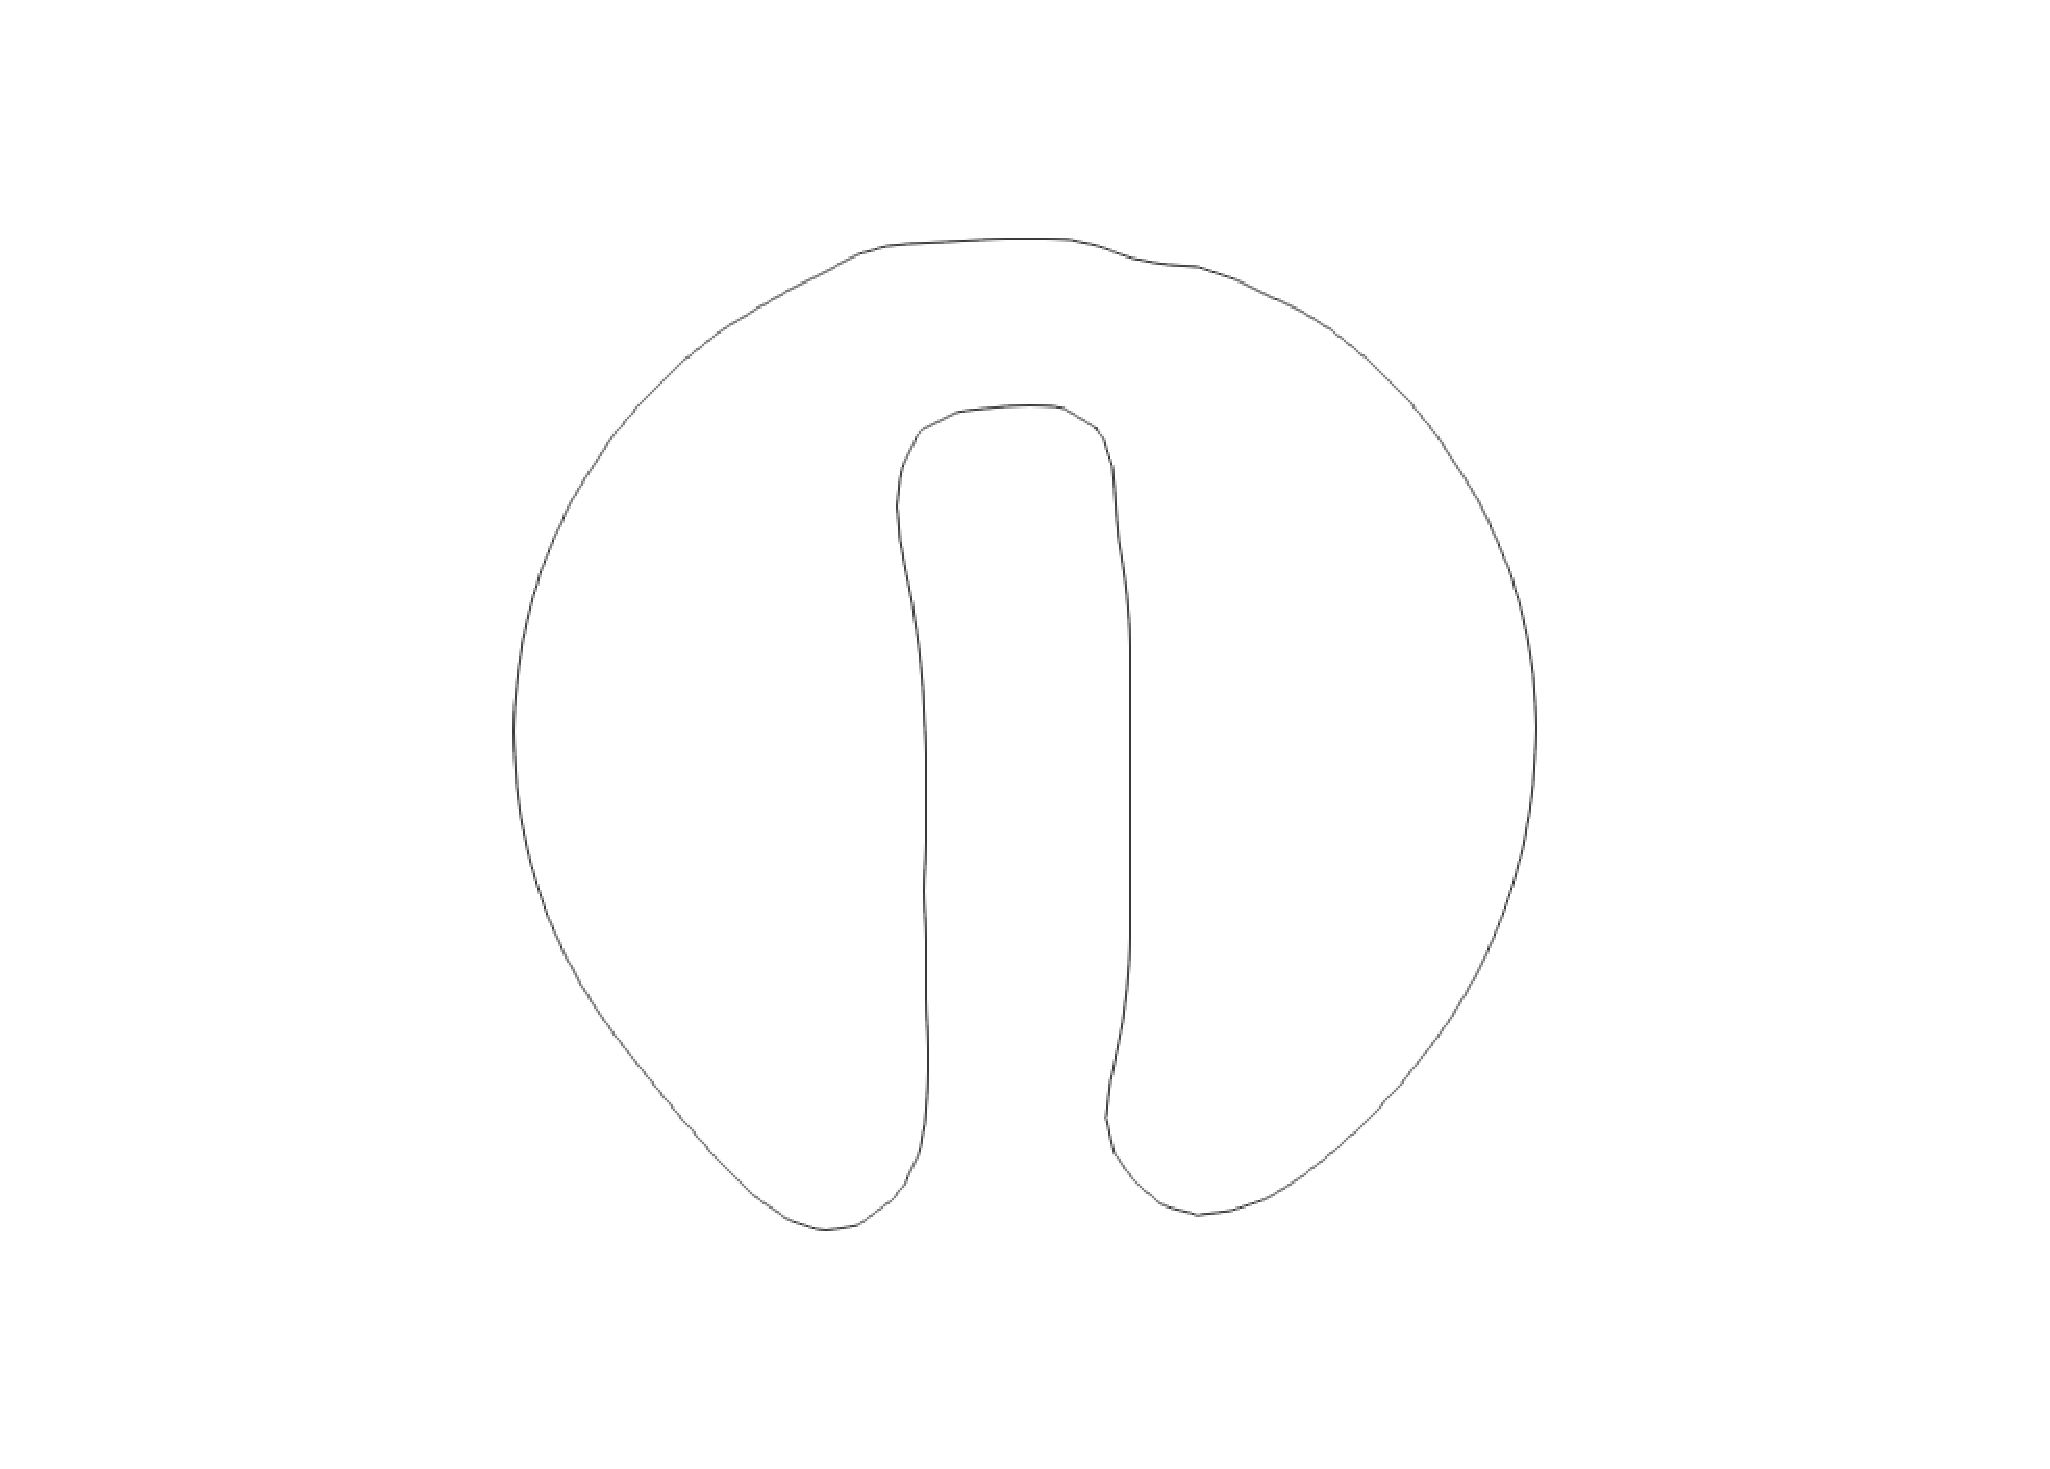
\includegraphics[width=0.3\textwidth]{CLSHexCo01coarse.eps}
\label{fig:CLSHexCo01coarse}
}
\subfigure[]{
\centering
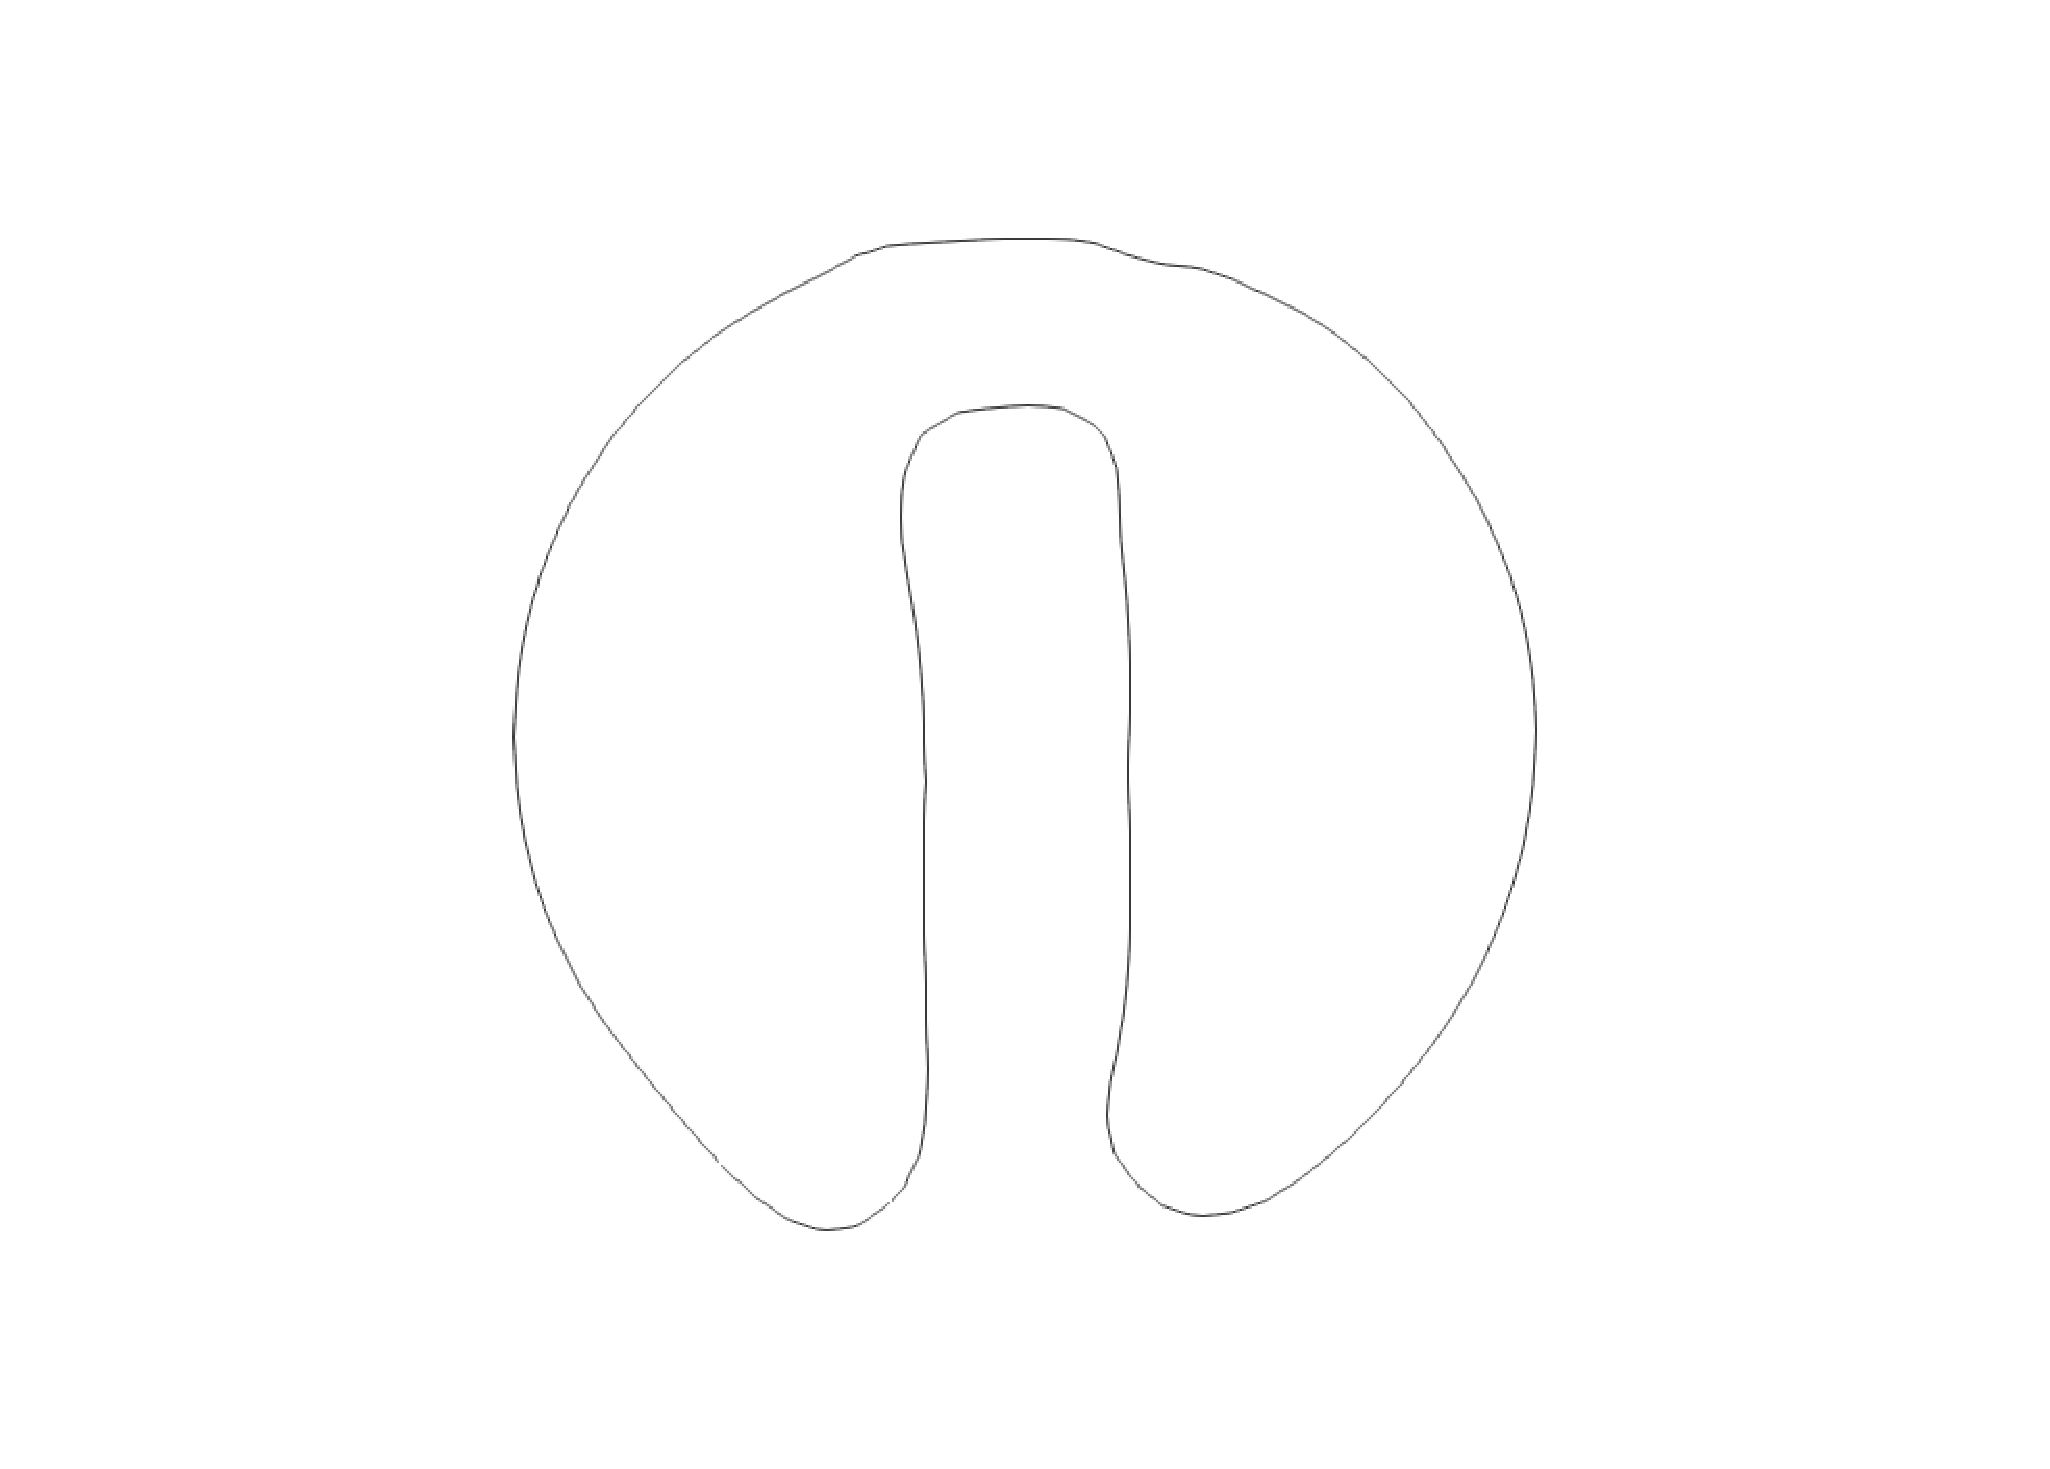
\includegraphics[width=0.3\textwidth]{CLSHexCo02coarse.eps}
\label{fig:CLSHexCo02coarse}
}
\subfigure[]{
\centering
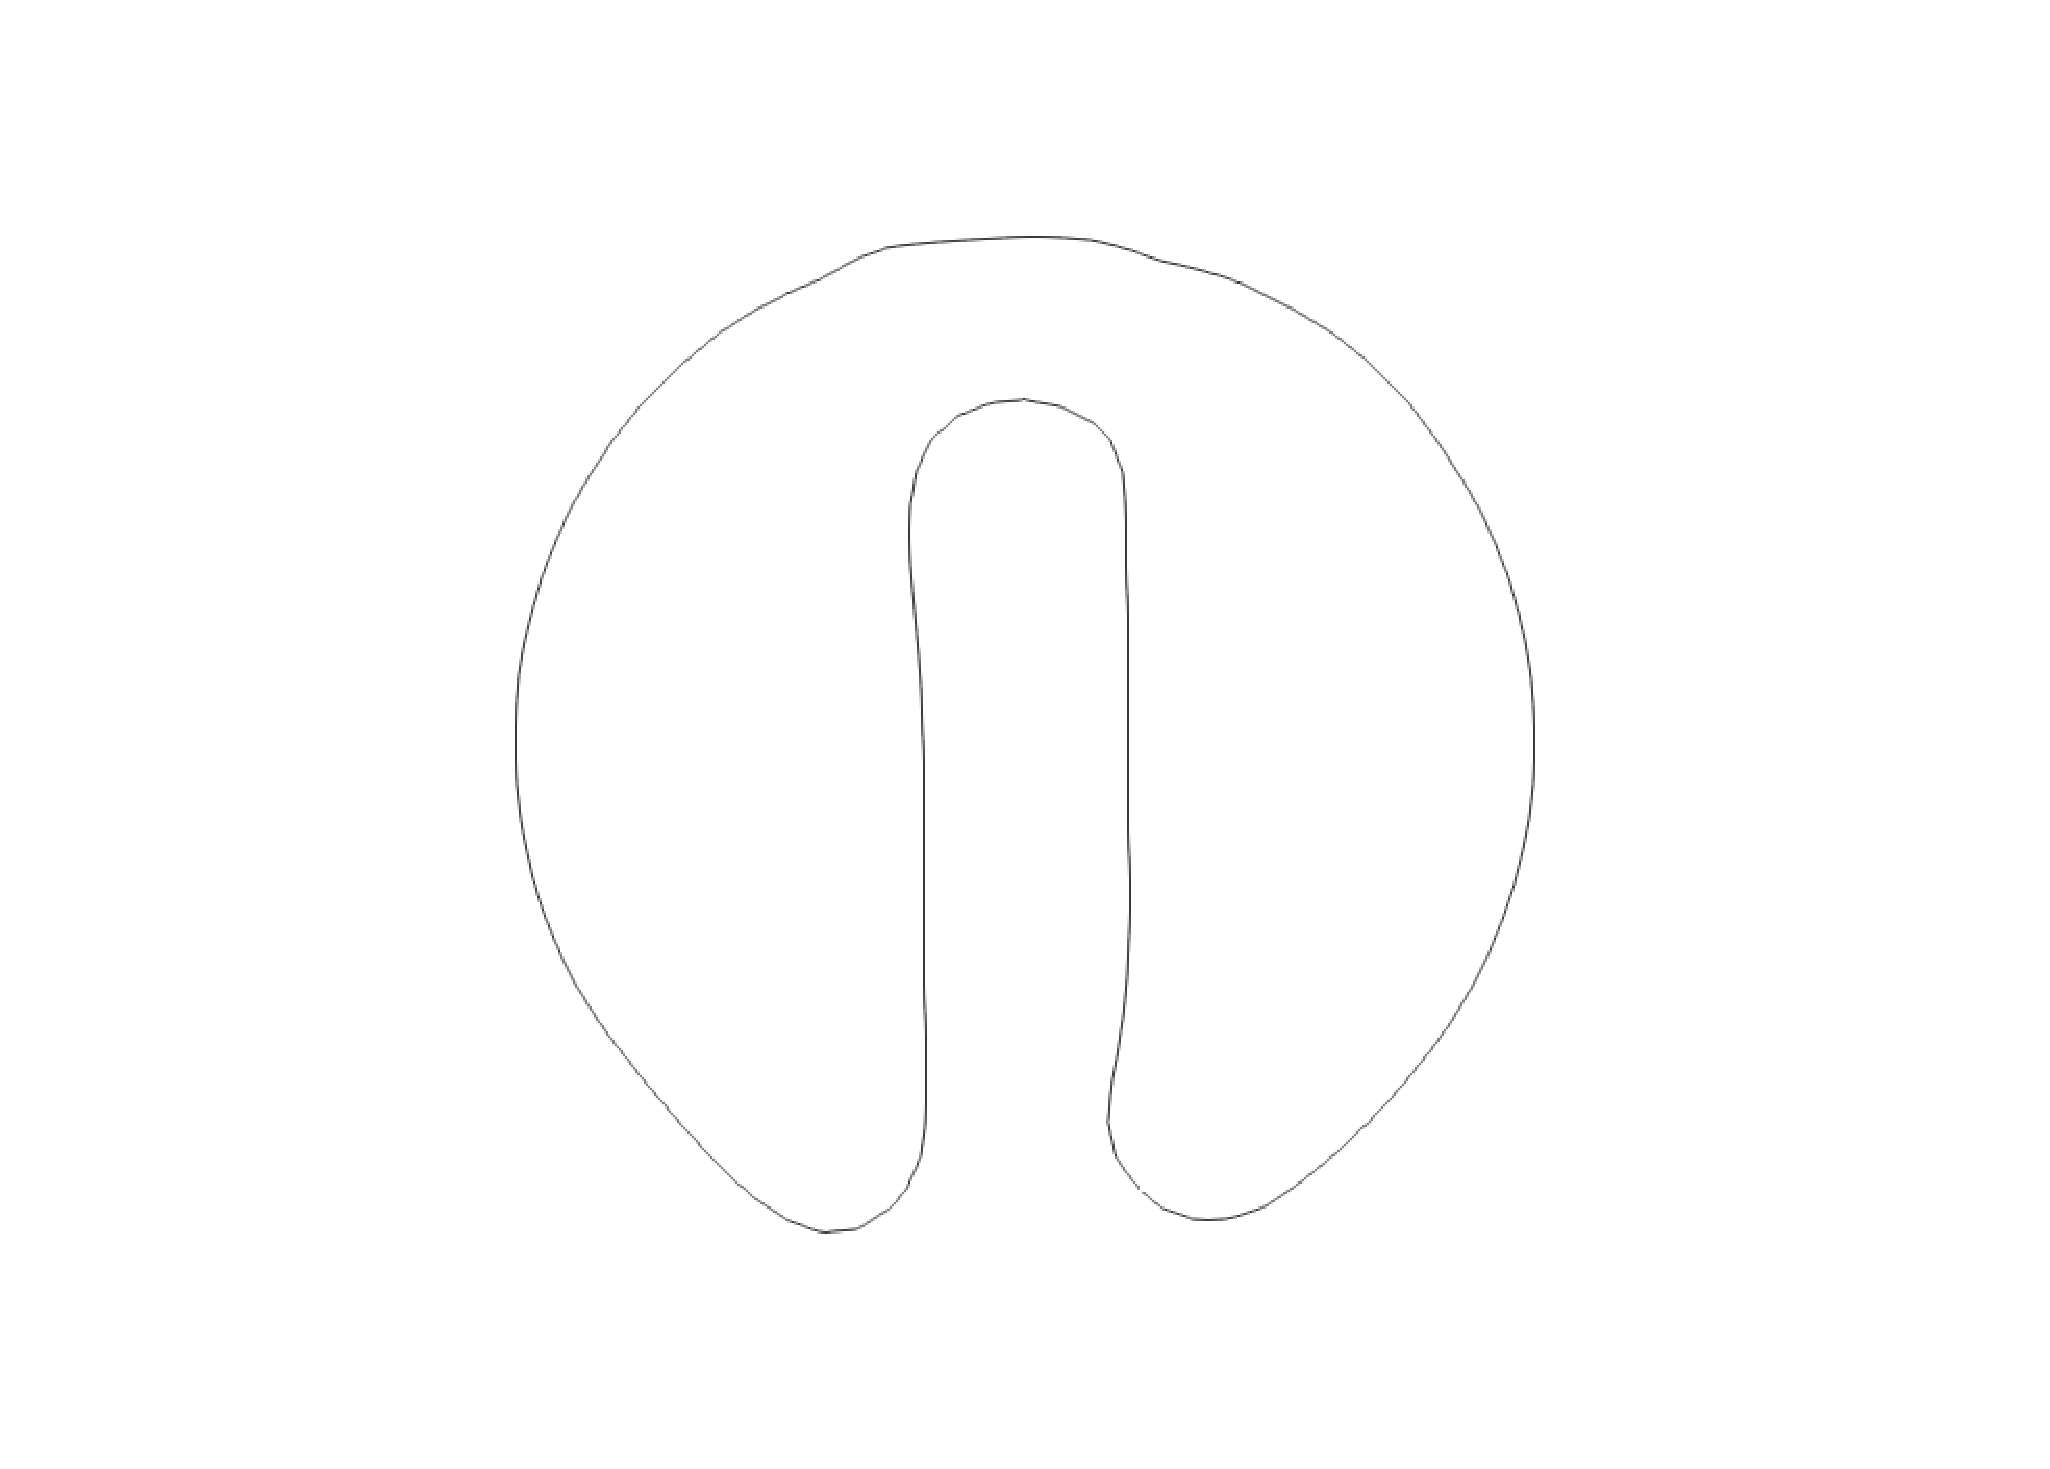
\includegraphics[width=0.3\textwidth]{CLSHexCo05coarse.eps}
\label{fig:CLSHexCo05coarse}
}
\subfigure[]{
\centering
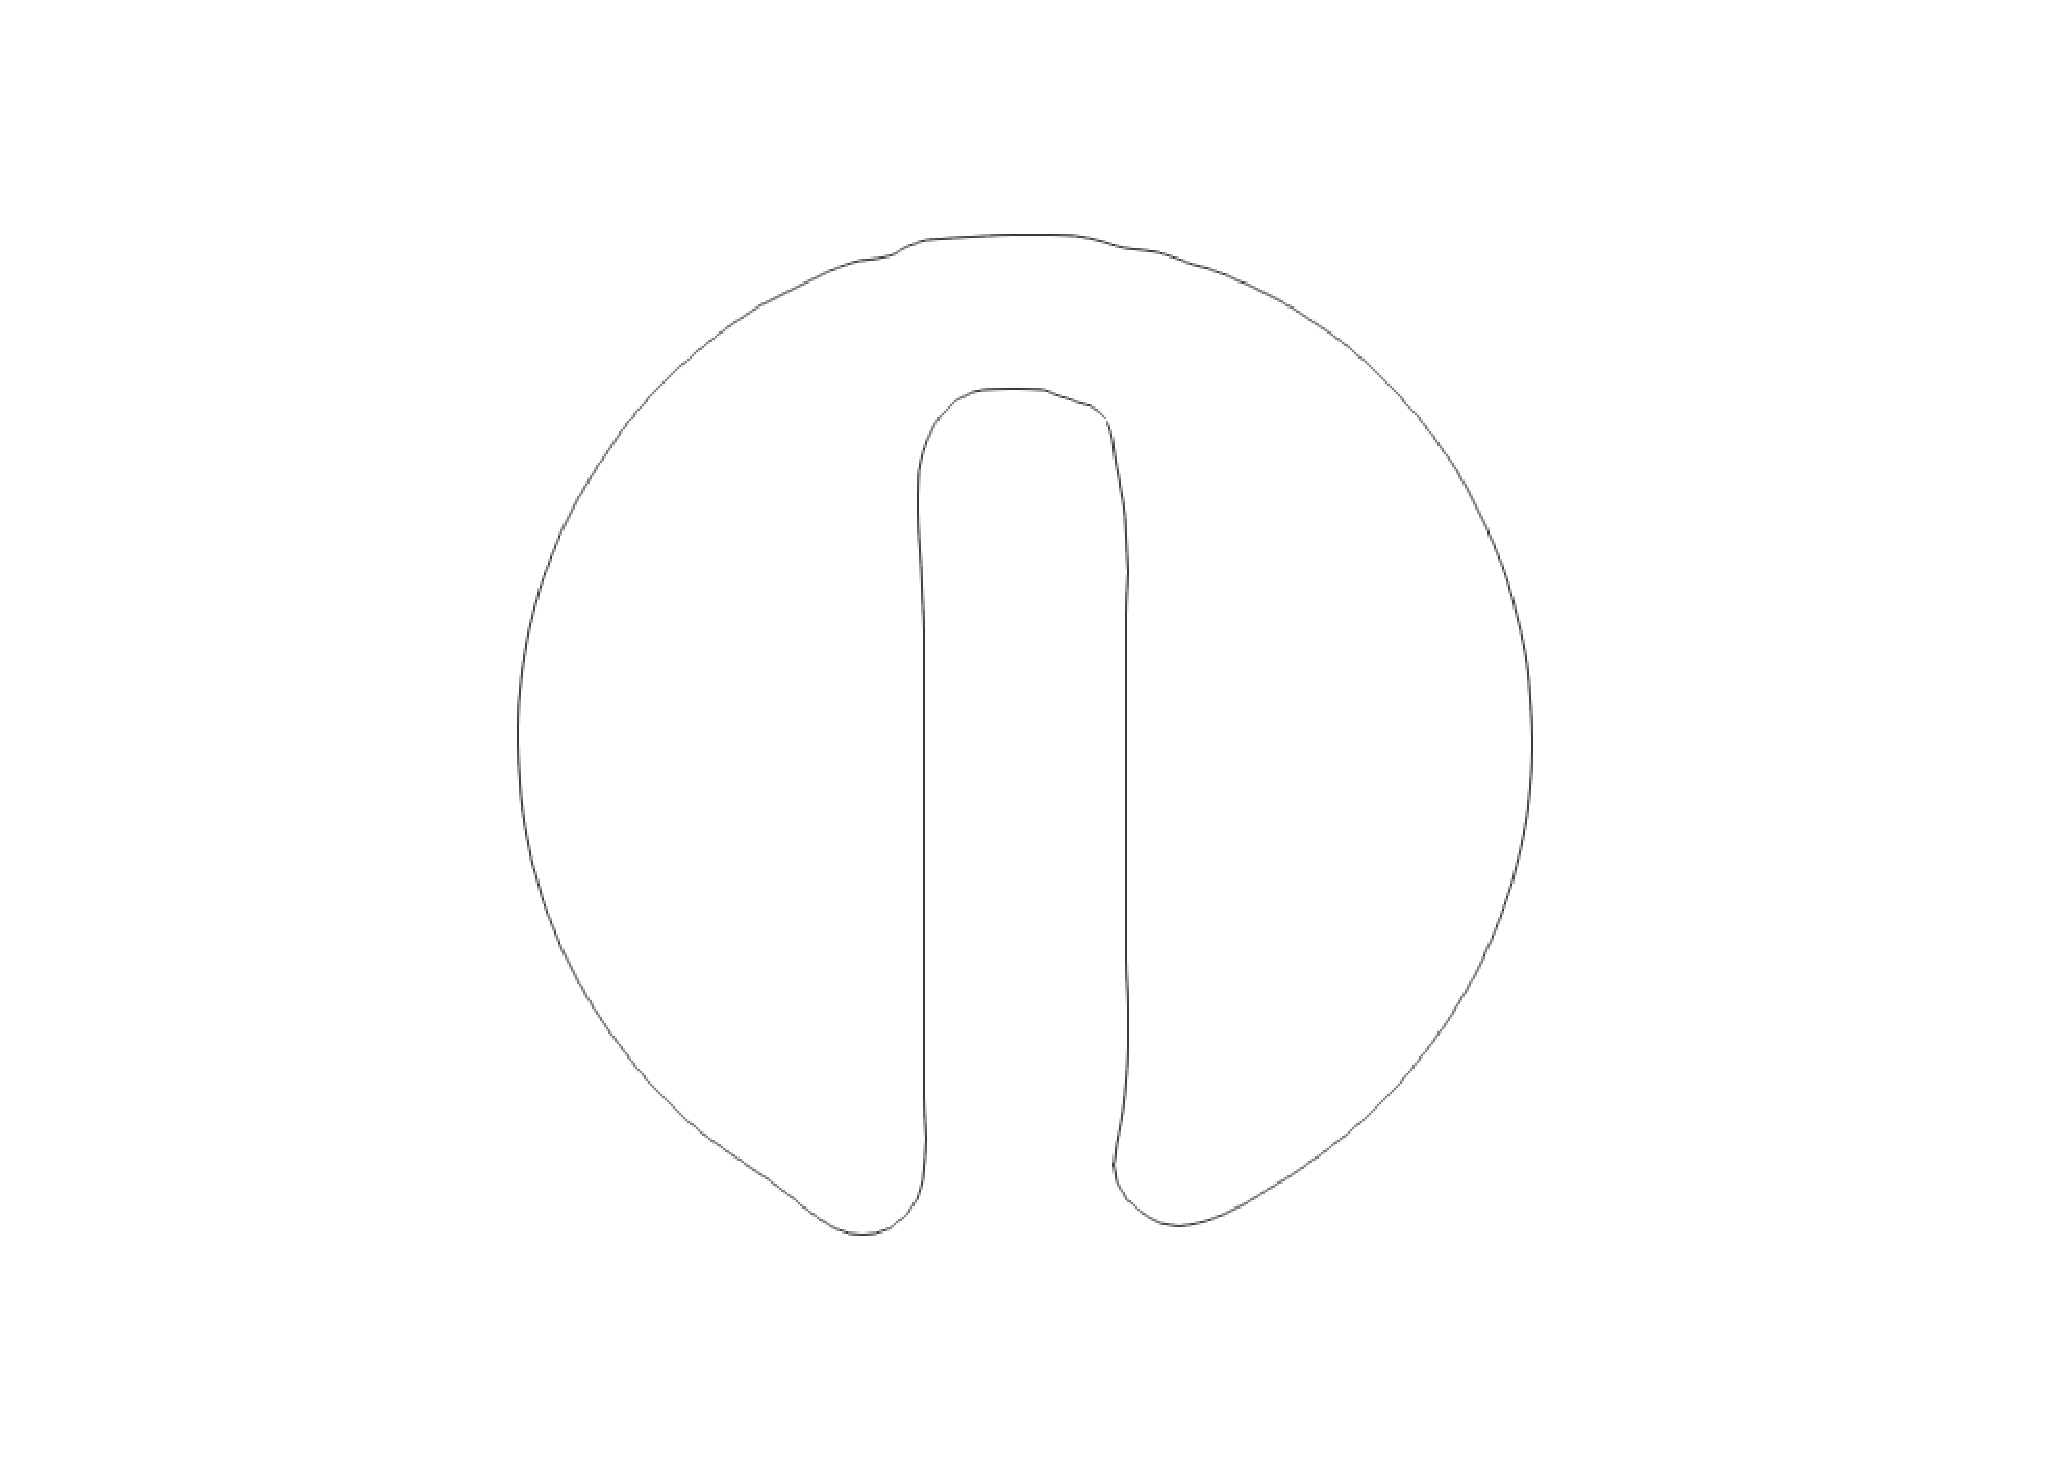
\includegraphics[width=0.3\textwidth]{CLSHexCo05mid.eps}
\label{fig:CLSHexCo05mid}
}
\subfigure[]{
\centering
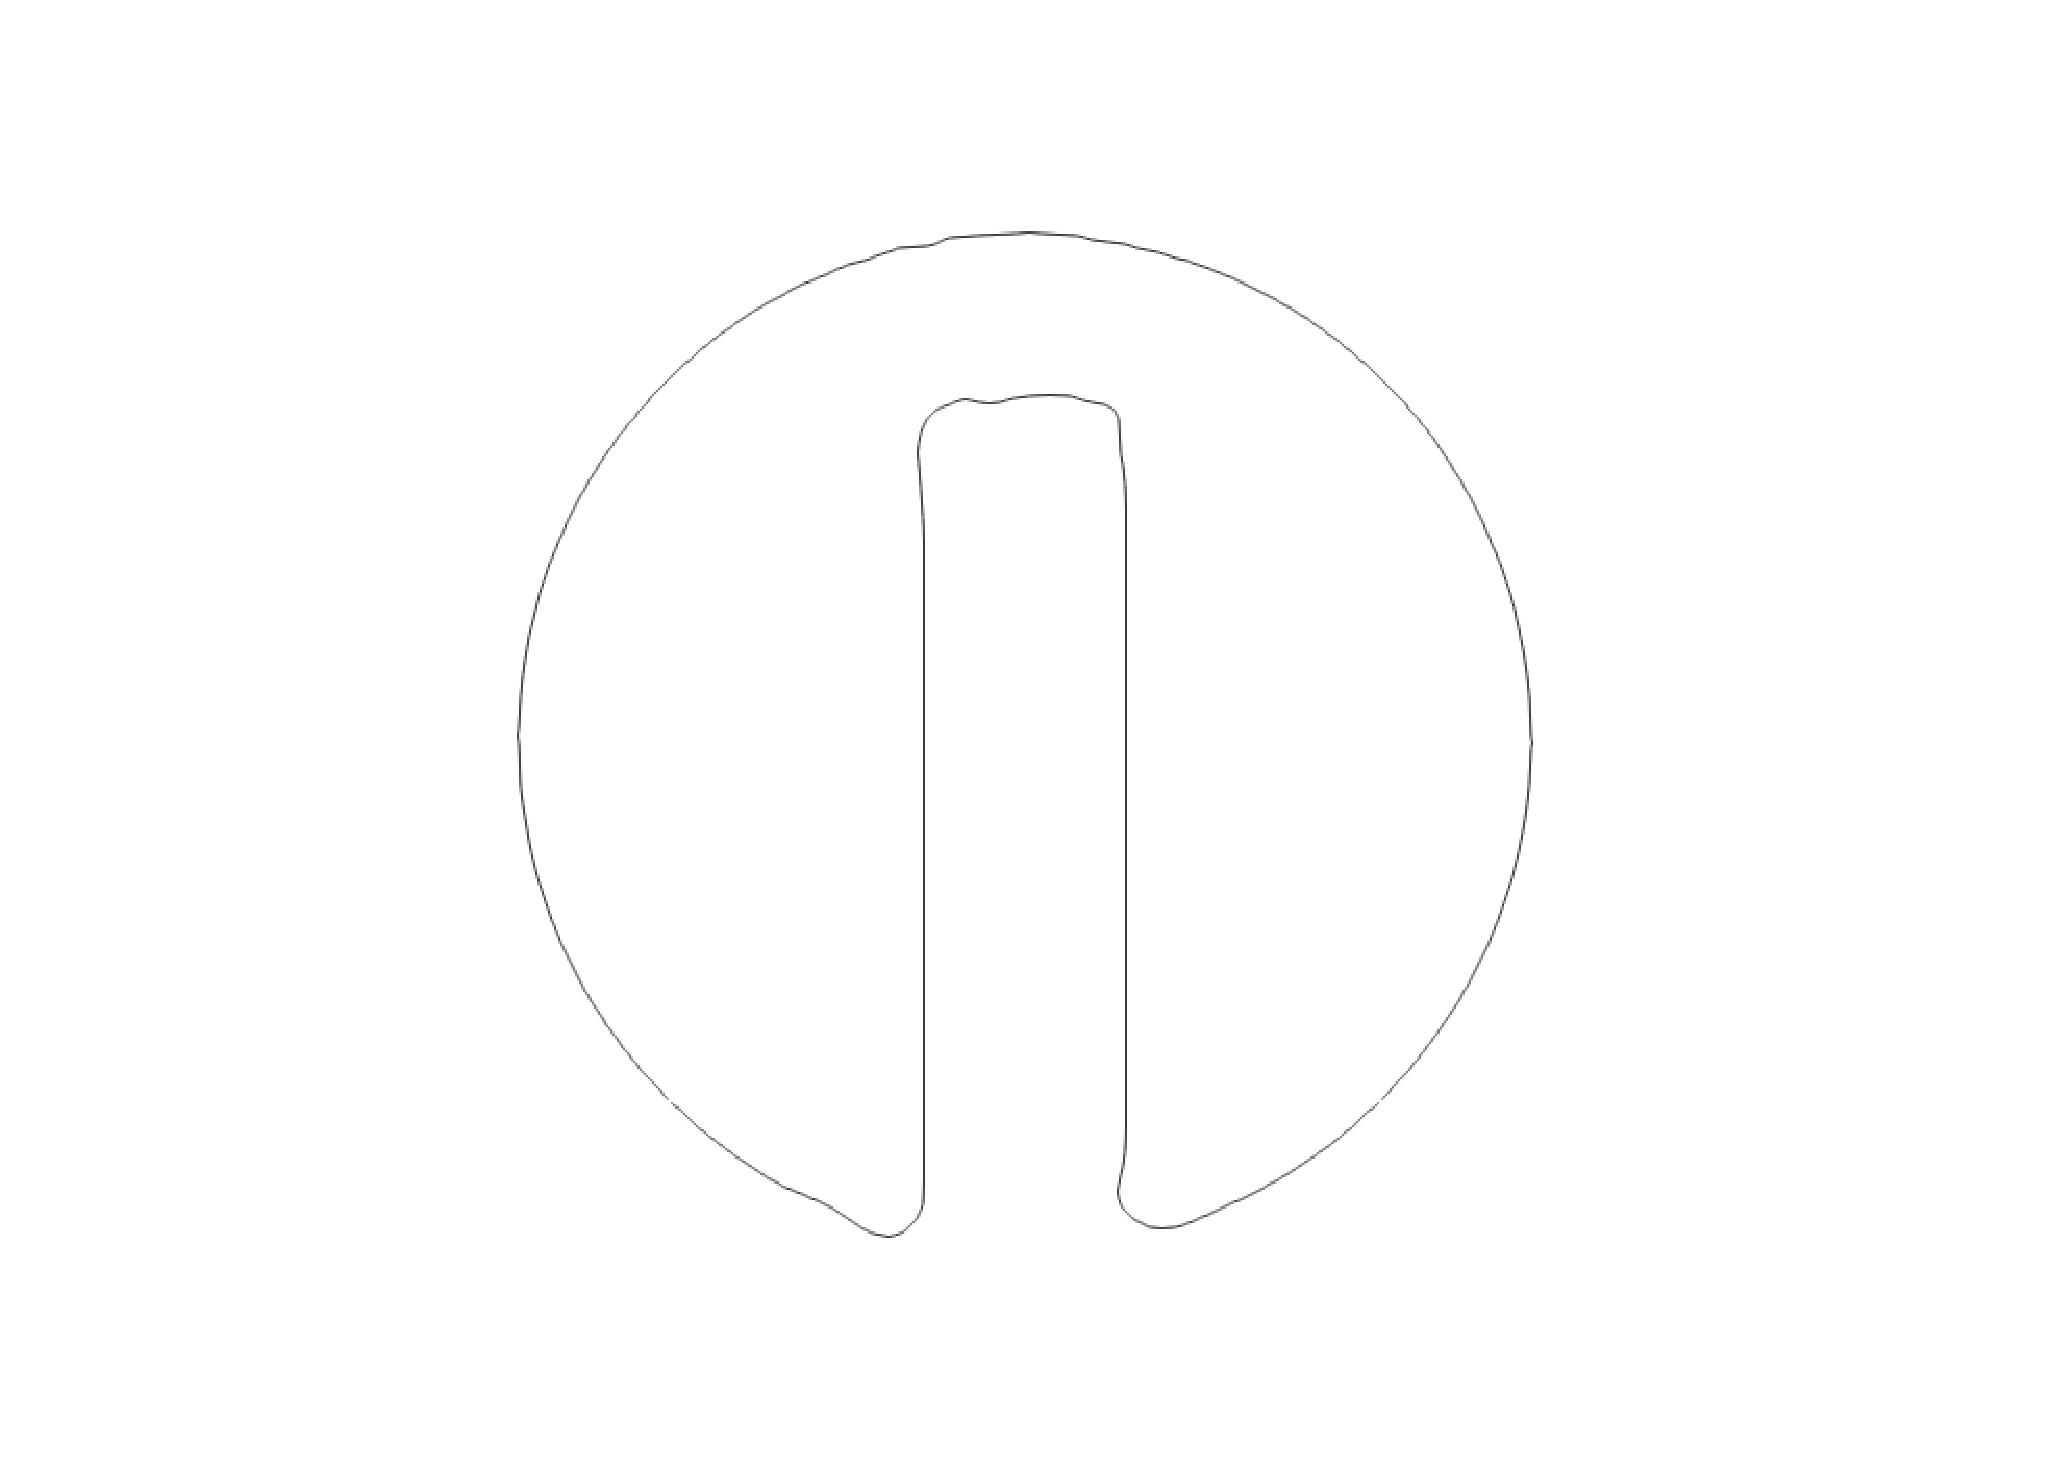
\includegraphics[width=0.3\textwidth]{CLSHexCo05fine.eps}
\label{fig:CLSHexCo05fine}
}
\caption{The shape after one circle with CLSAdvection method:\subref{fig:CLSHexCo01coarse} $100\times{100}$ and $Co=0.1$,\subref{fig:CLSHexCo02coarse} $100\times{100}$ and $Co=0.2$,\subref{fig:CLSHexCo05coarse} $100\times{100}$ and $Co=0.5$,\subref{fig:CLSHexCo05mid} $200\times{200}$ and $Co=0.5$,\subref{fig:CLSHexCo05fine} $400\times{400}$ and $Co=0.5$,}
\label{fig:CLSHEX}
\end{figure}
%%%%%%%%%%%%%%%%%%%%%%%%%%%%%%%%%%%%%%%%%%%%%%%%%%%%%%
\begin{figure}[htbp]
\centering
\subfigure[]{
\centering
\includegraphics[width=0.3\textwidth]{0_coarse_poly.eps}
%\caption{fig1}
\label{fig:polyCoarse}
}
\subfigure[]{
\centering
\includegraphics[width=0.3\textwidth]{0_mid_poly.eps}
\label{fig:polyMid}
%\caption{fig2}
}
\caption{Initial shape in polygon meshes with different cell numbers:\subref{fig:polyCoarse} 51967, \subref{fig:polyMid} 203965}
\label{fig:poly0}
\end{figure}
%%%%%%%%%%%%%%%%%%%%%%%%%%%%%%%%%%%%%%%%%%%%%%%%%%%%%%
\begin{figure}[htbp]
\centering
\subfigure[]{
\centering
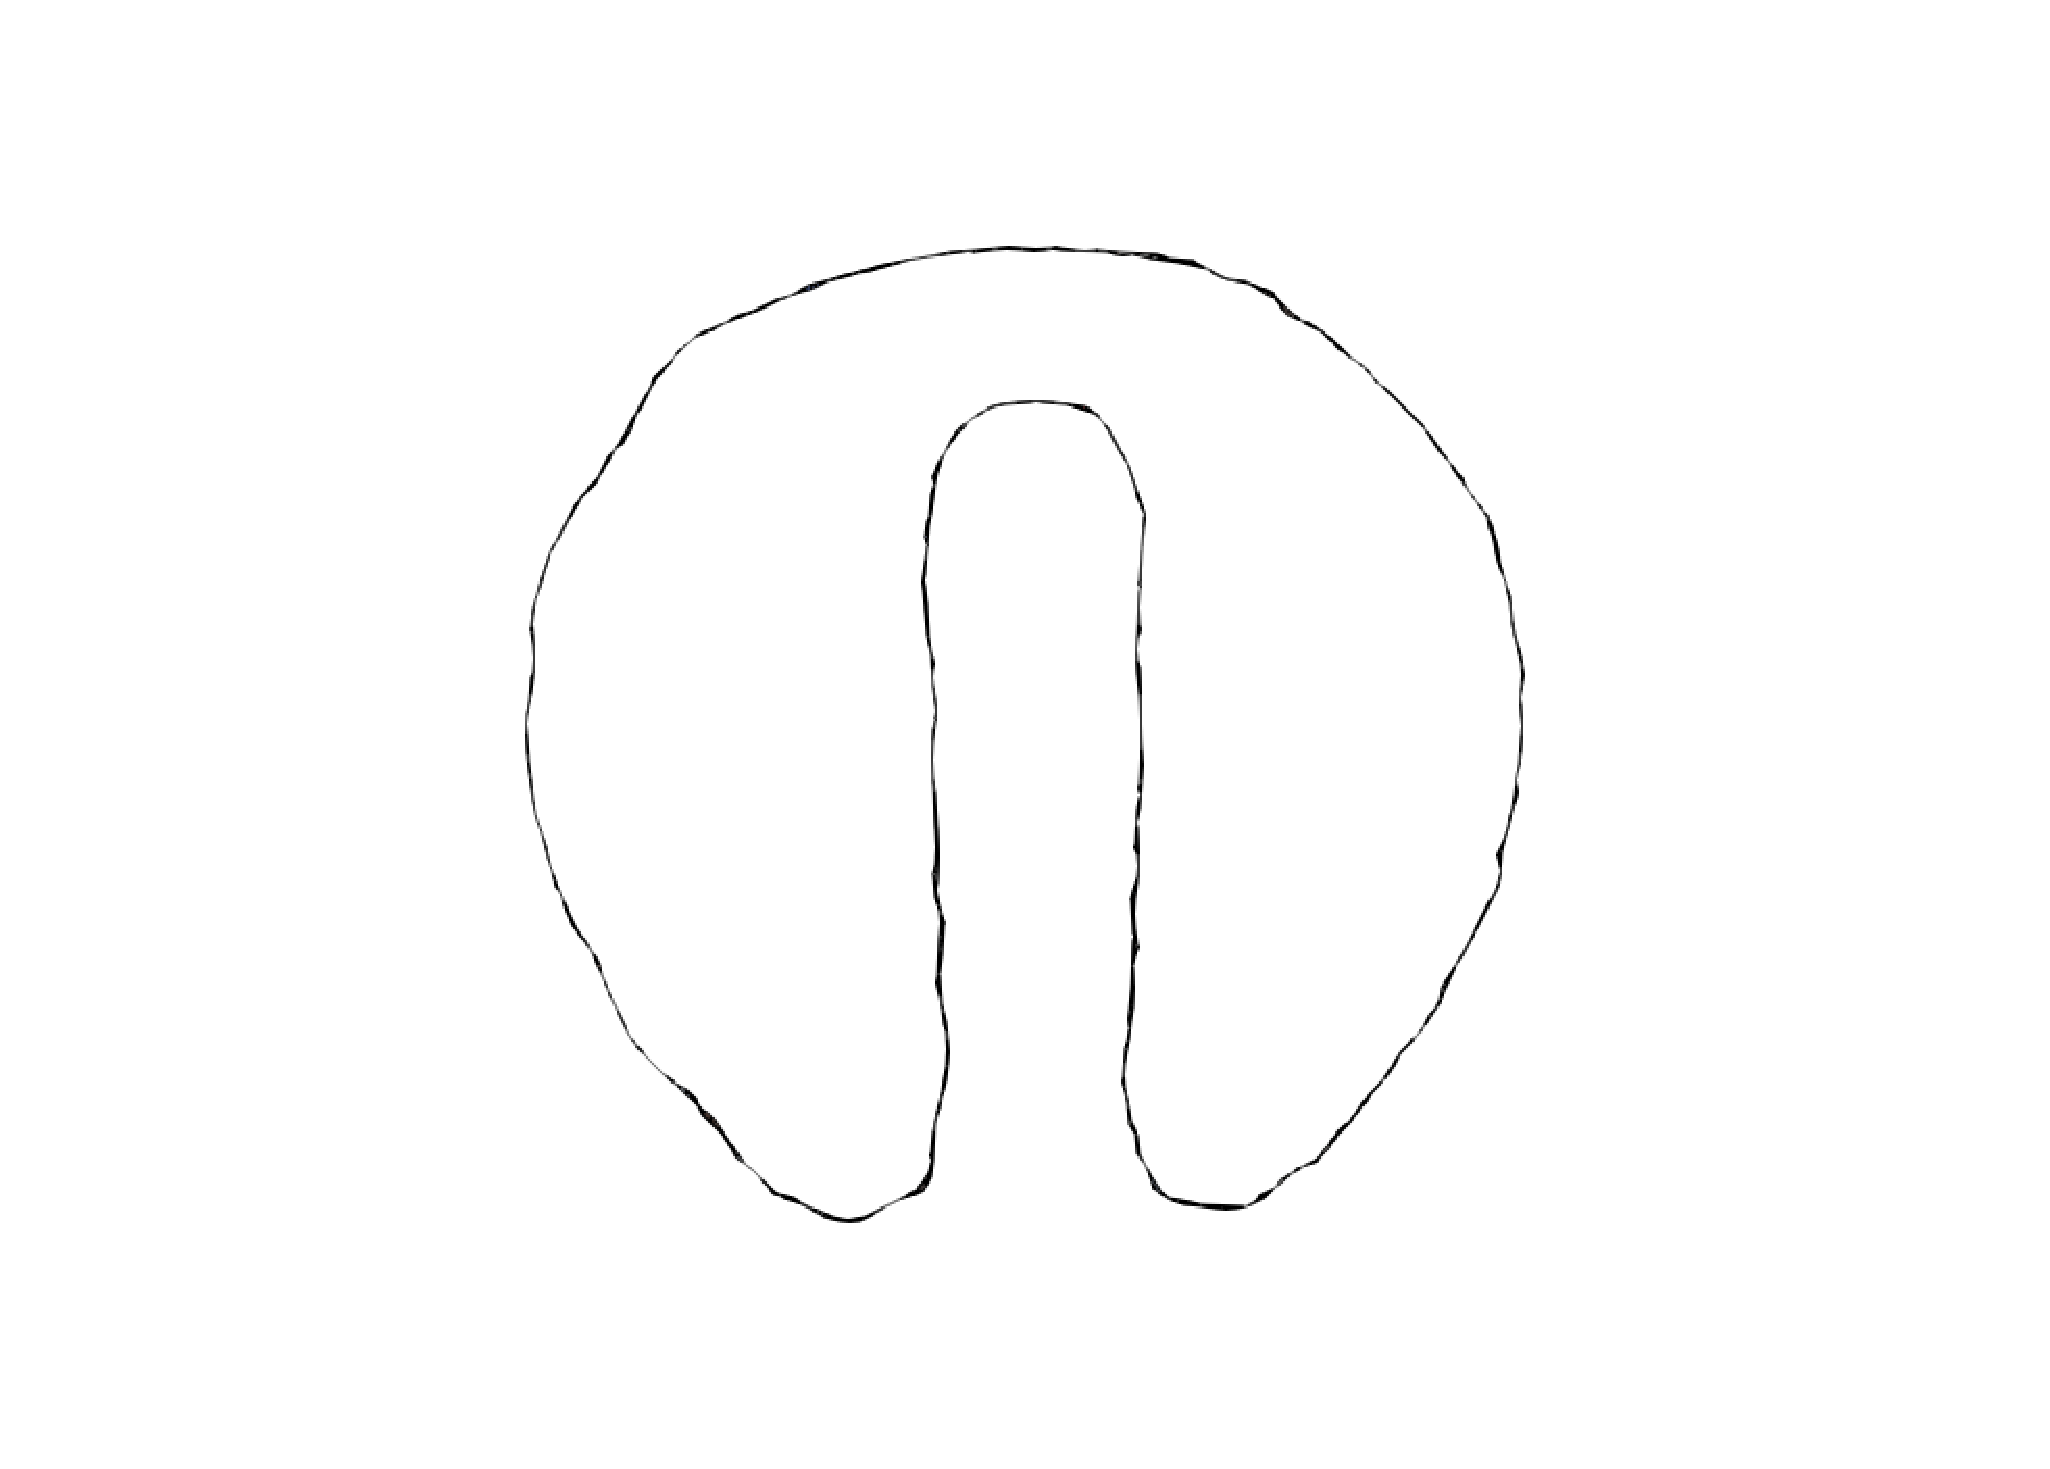
\includegraphics[width=0.3\textwidth]{MULESPolyCo01Coarse.eps}
%\caption{fig1}
\label{fig:MULESPolyCo01Coarse}
}
\subfigure[]{
\centering
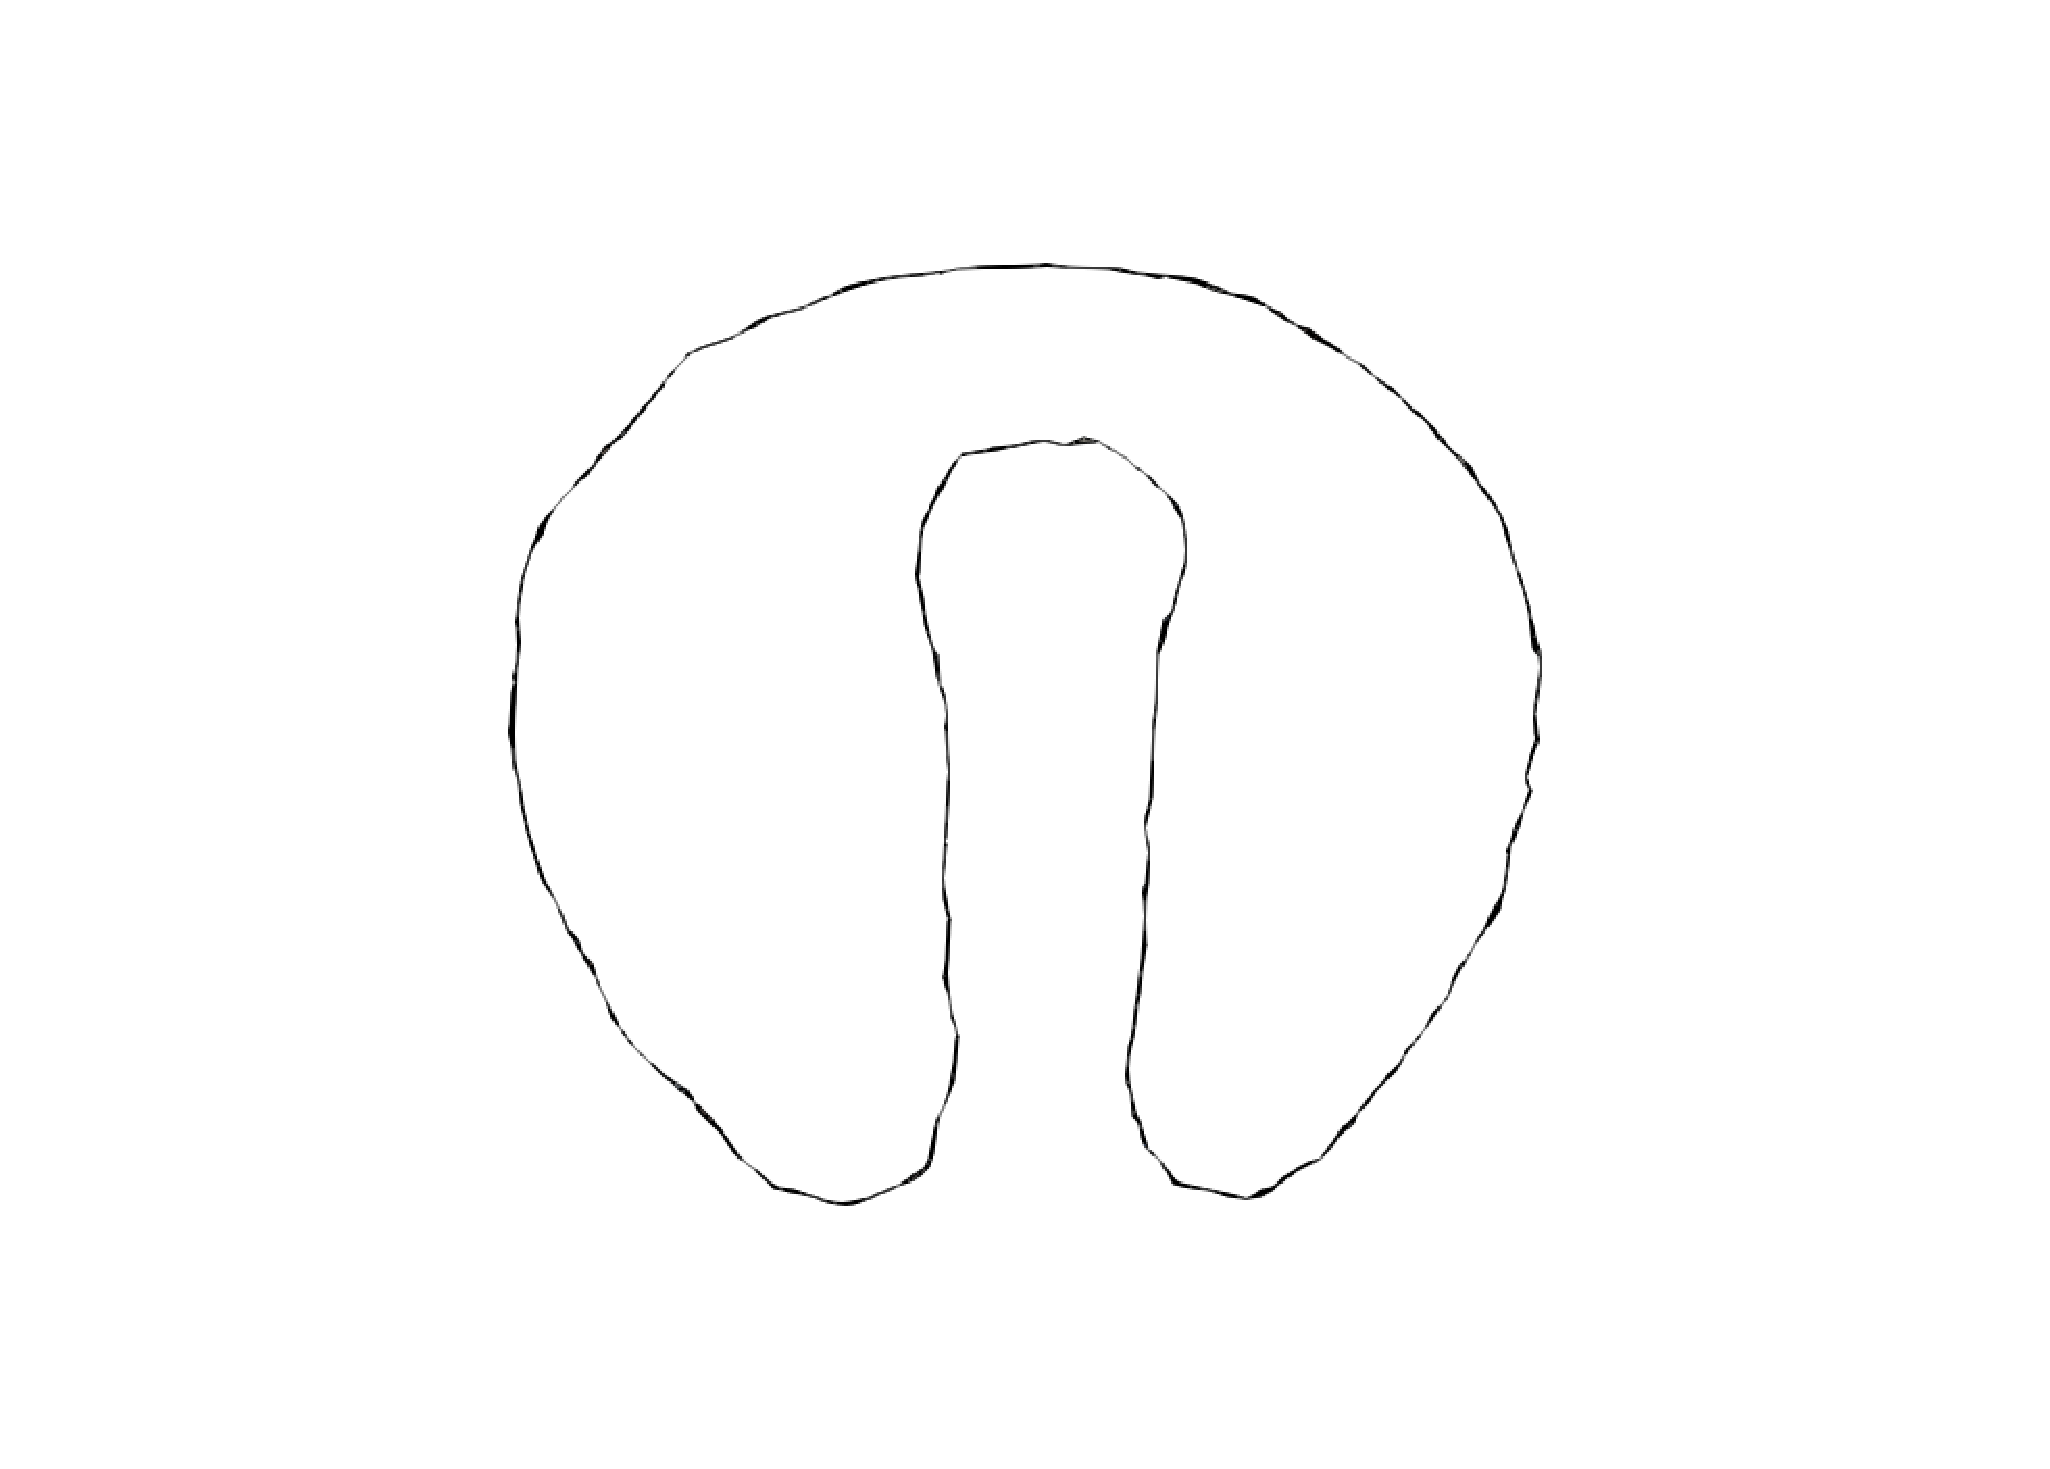
\includegraphics[width=0.3\textwidth]{MULESPolyCo05Coarse.eps}
%\caption{fig1}
\label{fig:MULESPolyCo05Coarse}
}
\subfigure[]{
\centering
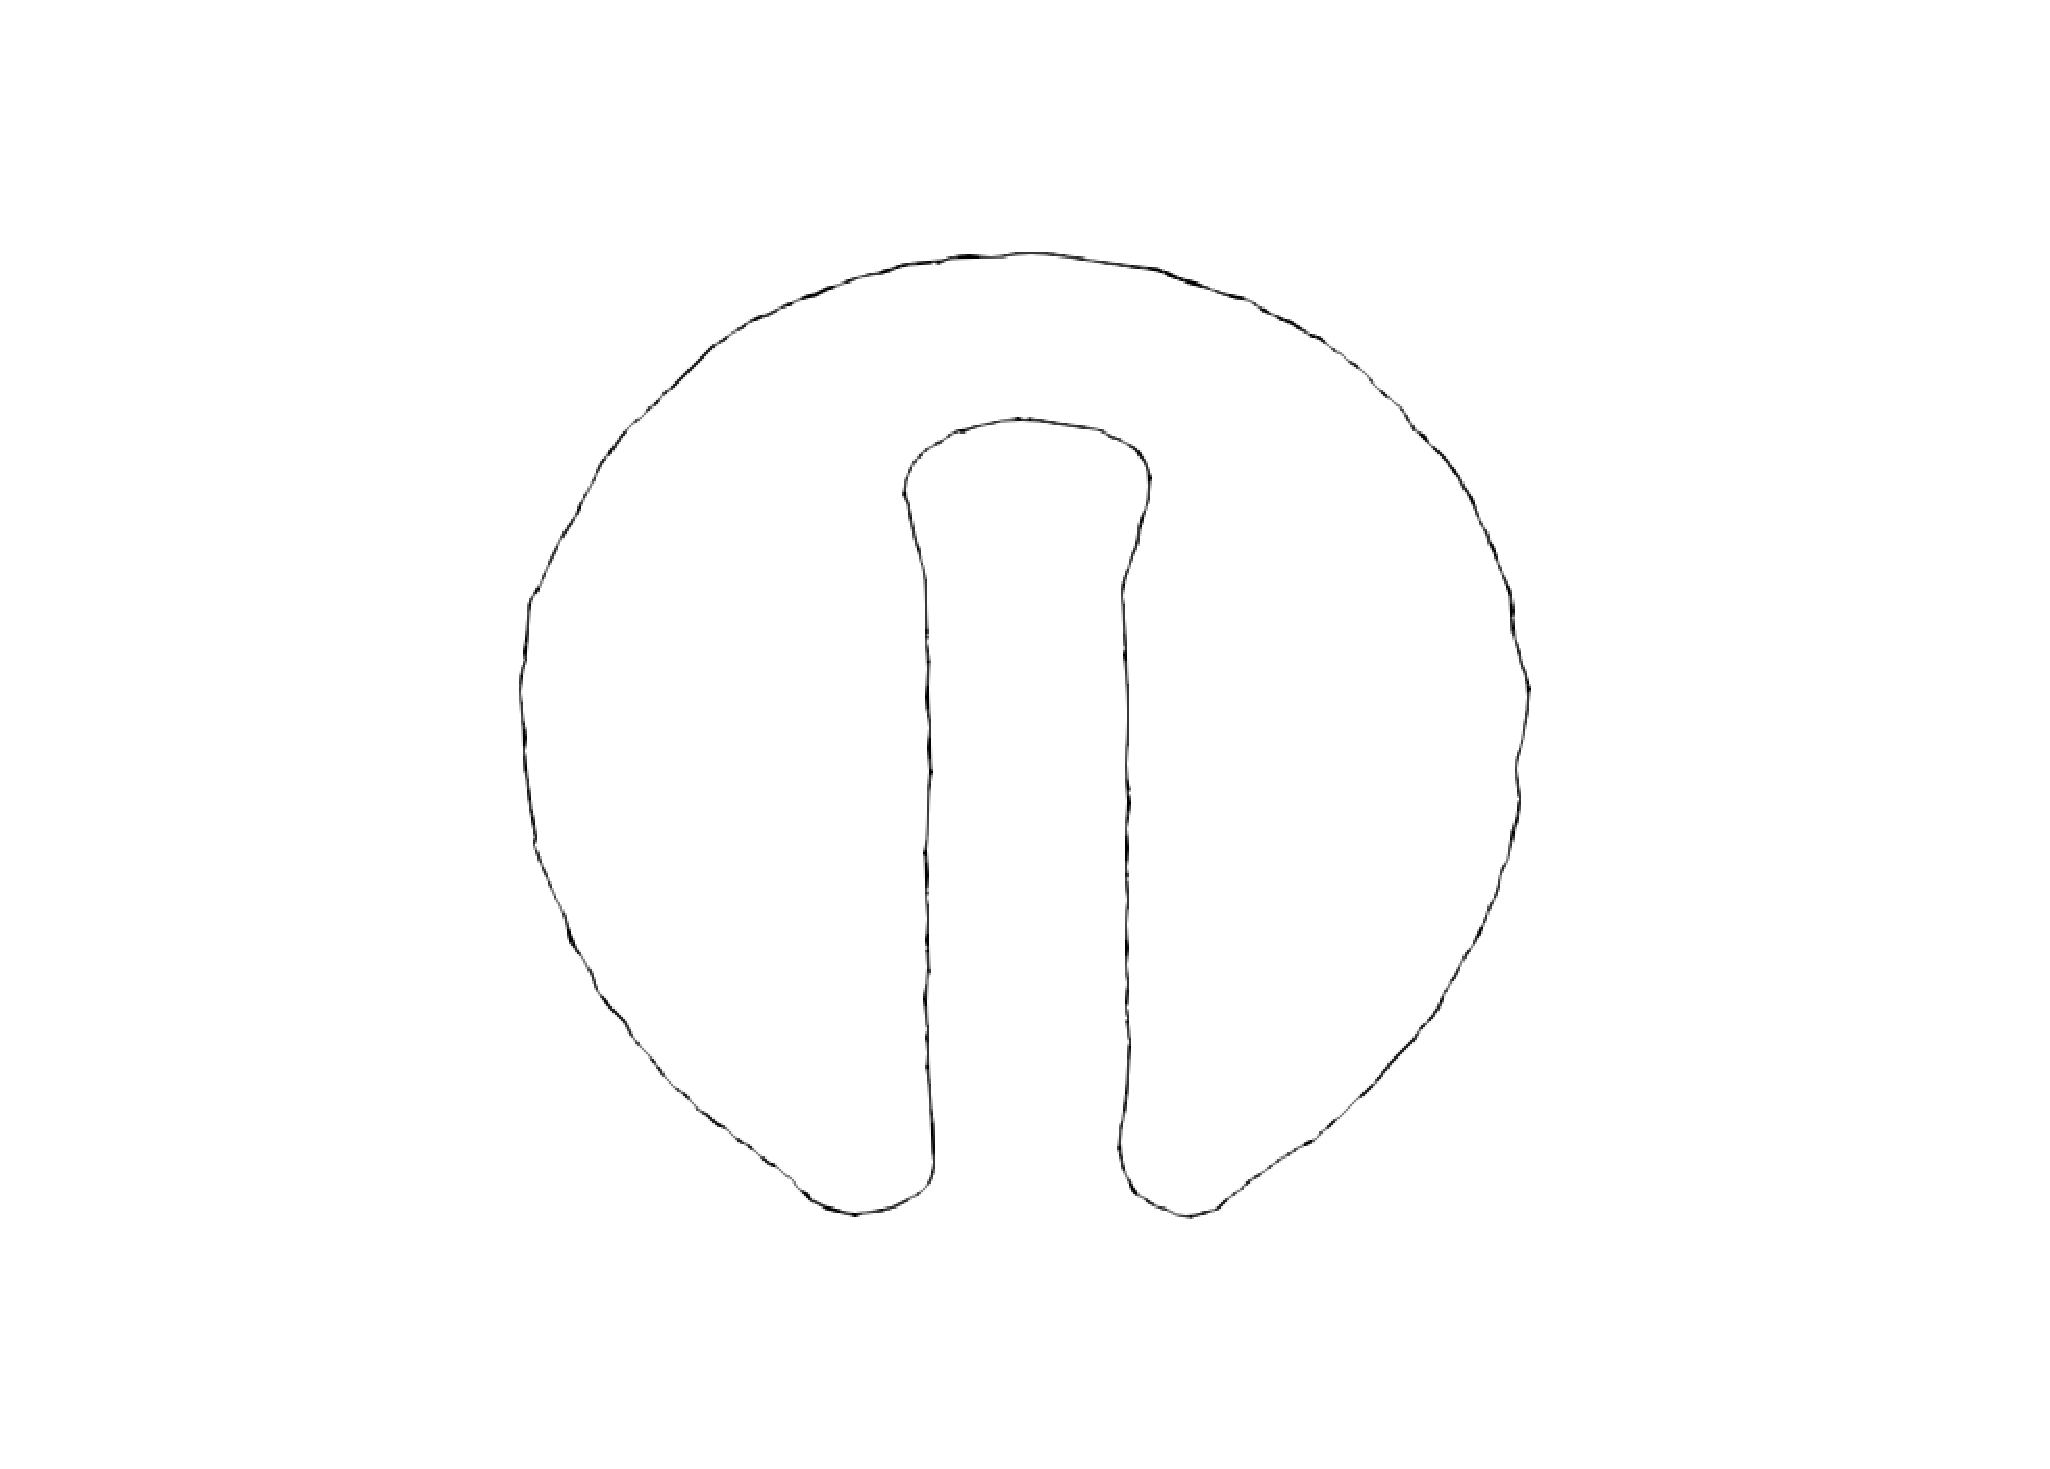
\includegraphics[width=0.3\textwidth]{MULESPolyCo05Mid.eps}
\label{fig:MULESPolyCo05Mid}
%\caption{fig2}
}
\caption{The shape after one circle with MULSE method:\subref{fig:MULESPolyCo01Coarse} 51967 and $Co=0.1$, \subref{fig:MULESPolyCo05Coarse} 51967 and $Co=0.5$,\subref{fig:MULESPolyCo05Mid} 203965 and $Co=0.5$}
\label{fig:MULESPoly}
\end{figure}
%%%%%%%%%%%%%%%%%%%%%%%%%%%%%%%%%%%%%%%%%%%%%%%%%%%%
\begin{figure}[htbp]
\centering
\subfigure[]{
\centering
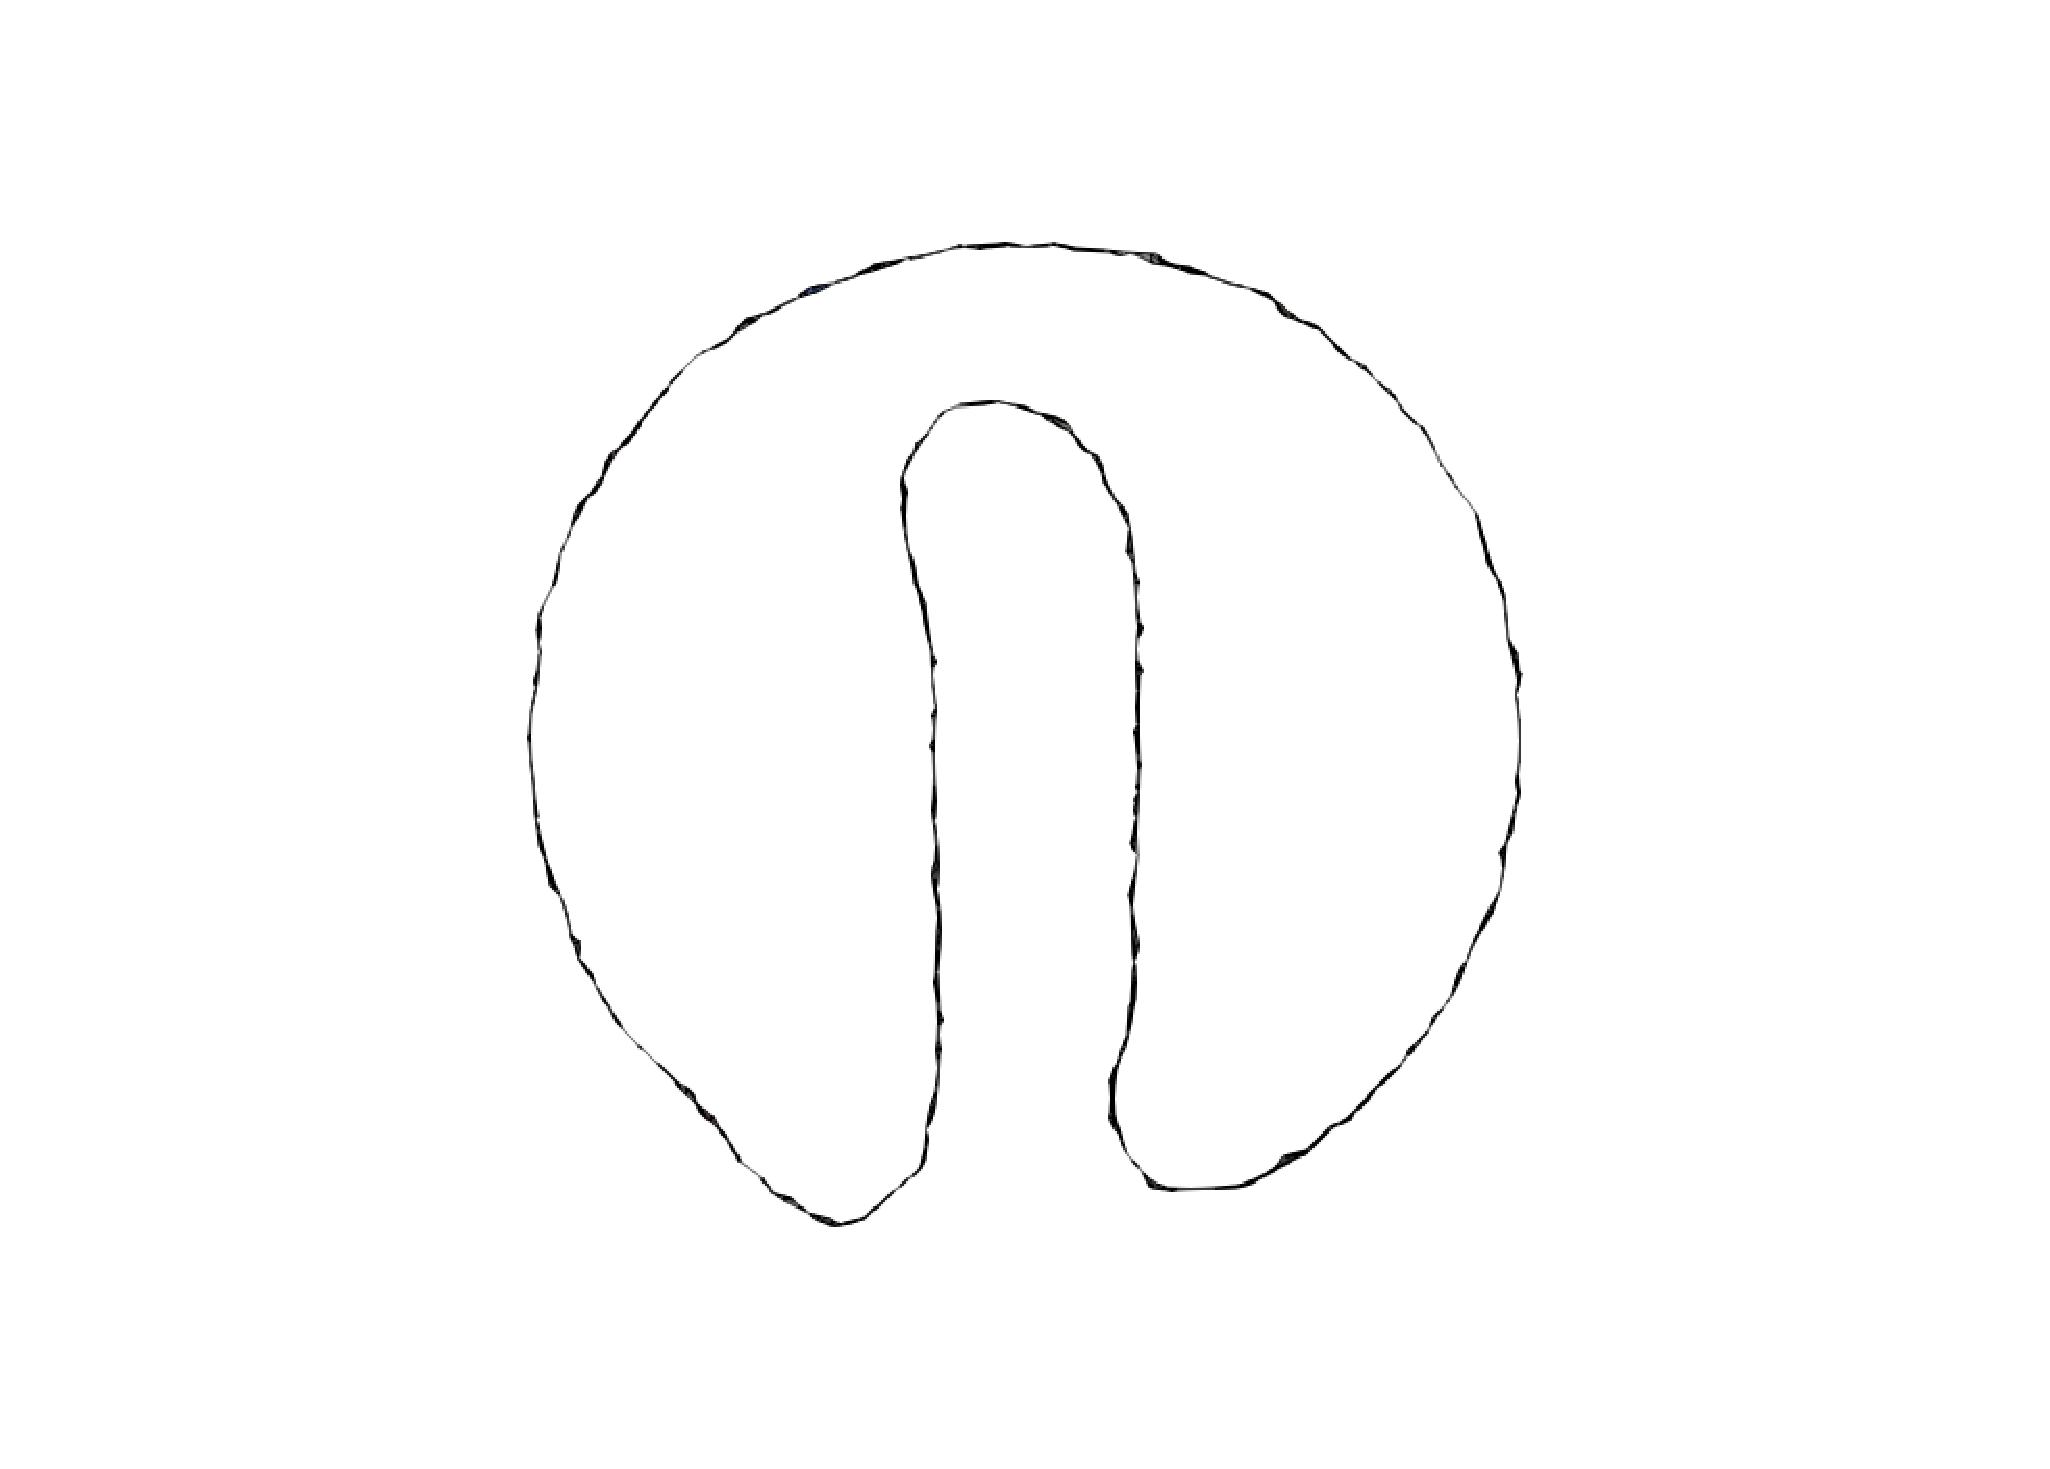
\includegraphics[width=0.3\textwidth]{ISOPolyCo01Coarse.eps}
%\caption{fig1}
\label{fig:ISOPolyCo01Coarse}
}
\subfigure[]{
\centering
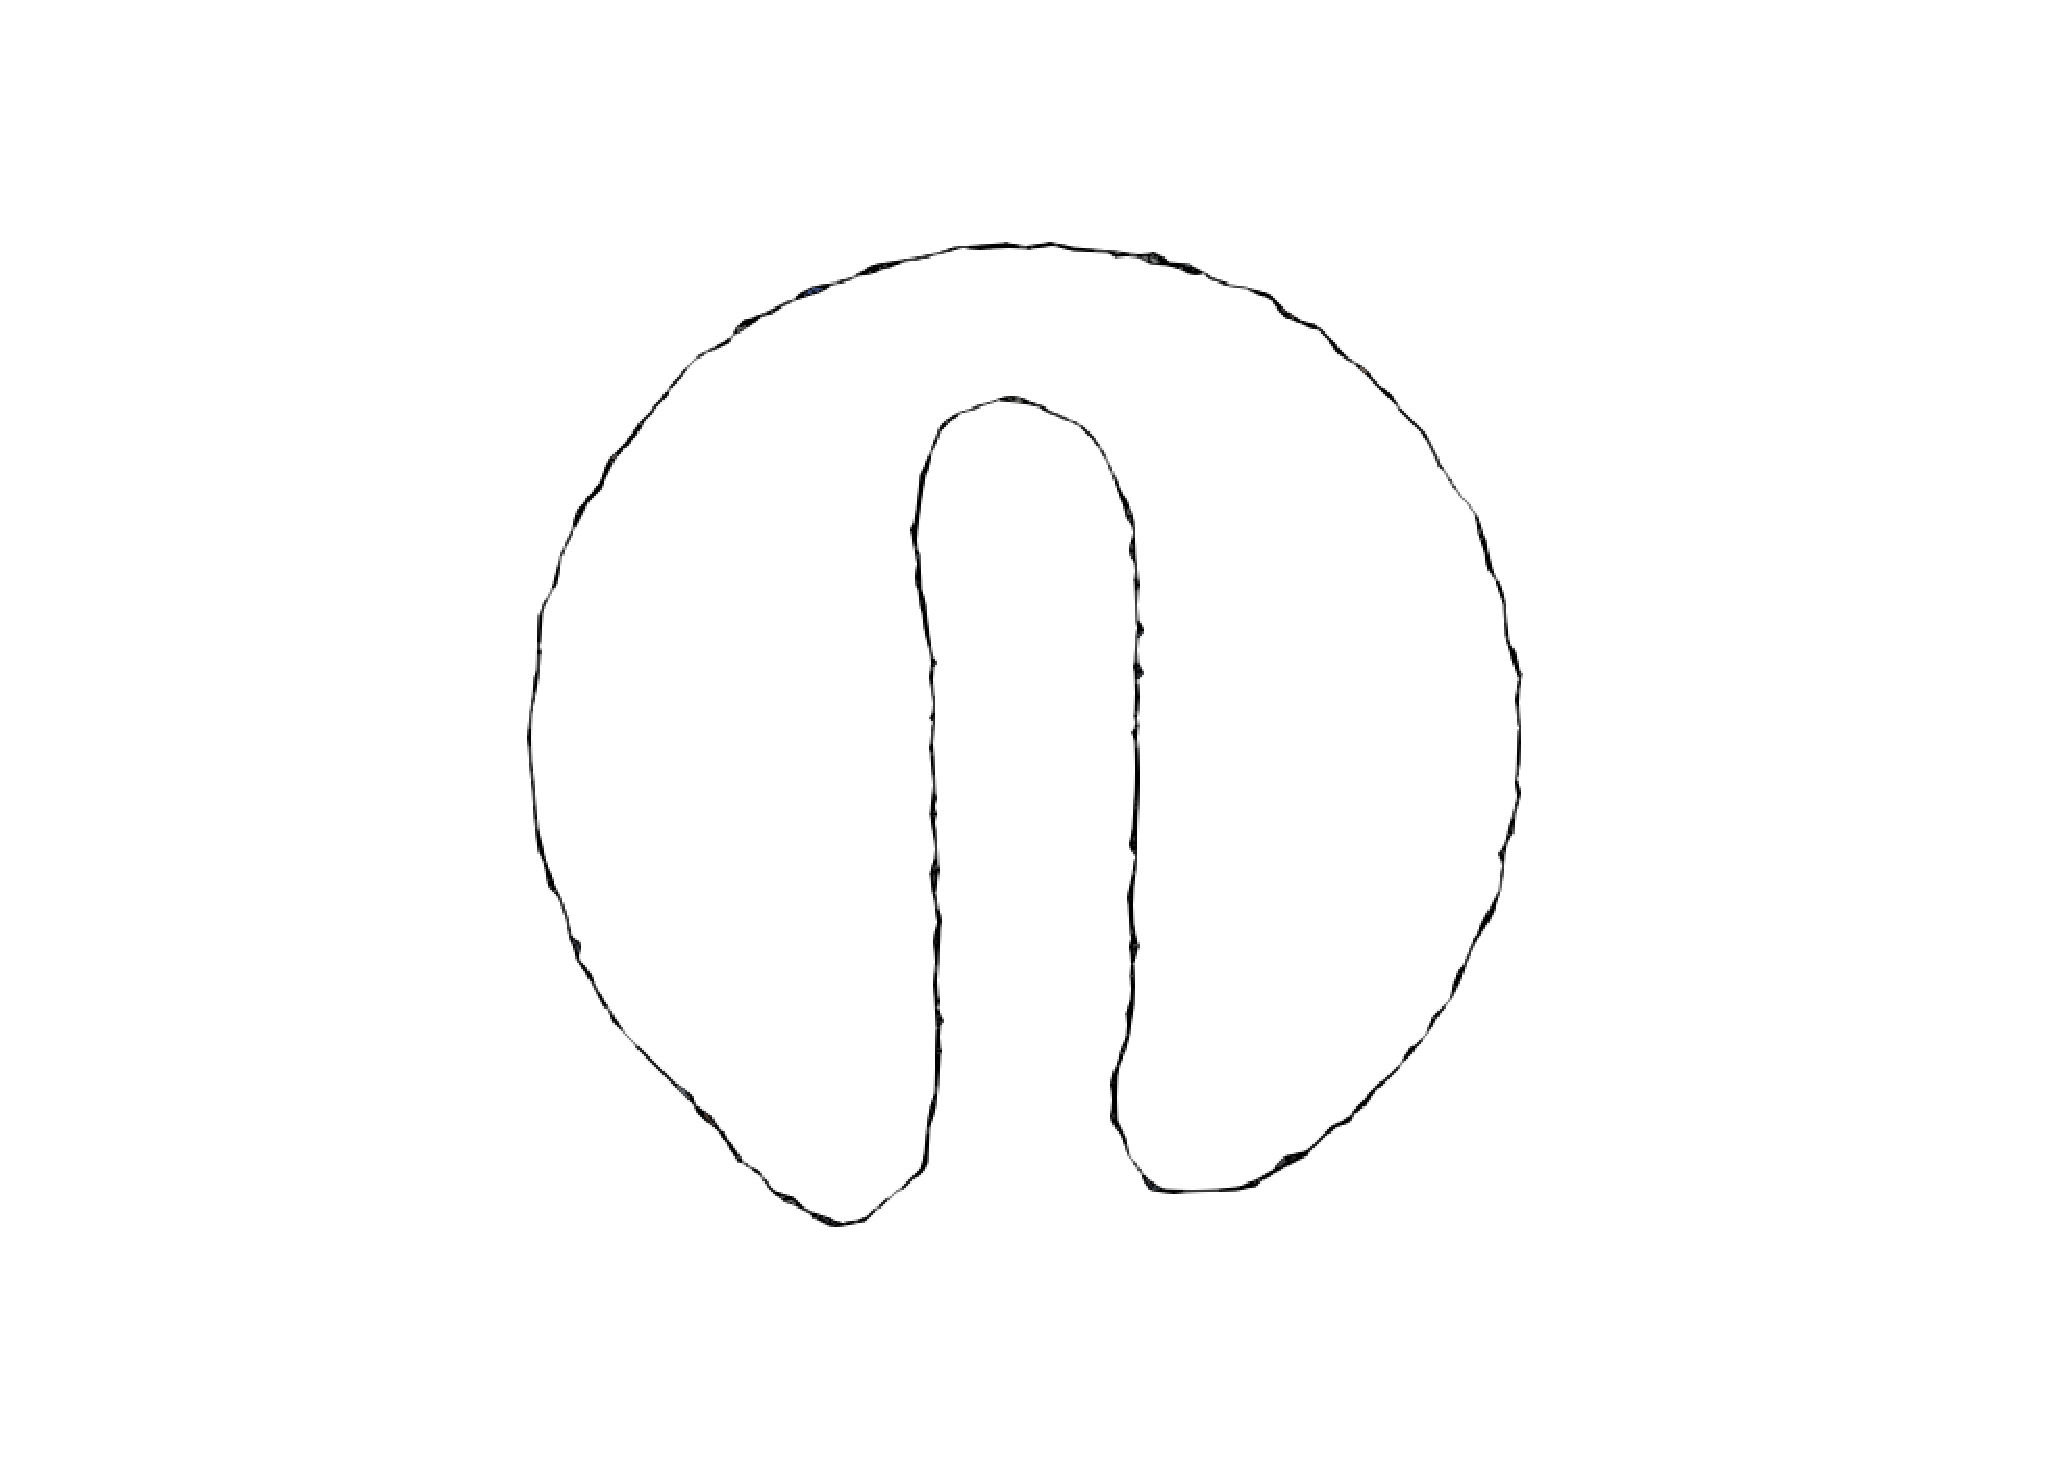
\includegraphics[width=0.3\textwidth]{ISOPolyCo05Coarse.eps}
%\caption{fig1}
\label{fig:ISOPolyCo05Coarse}
}
\subfigure[]{
\centering
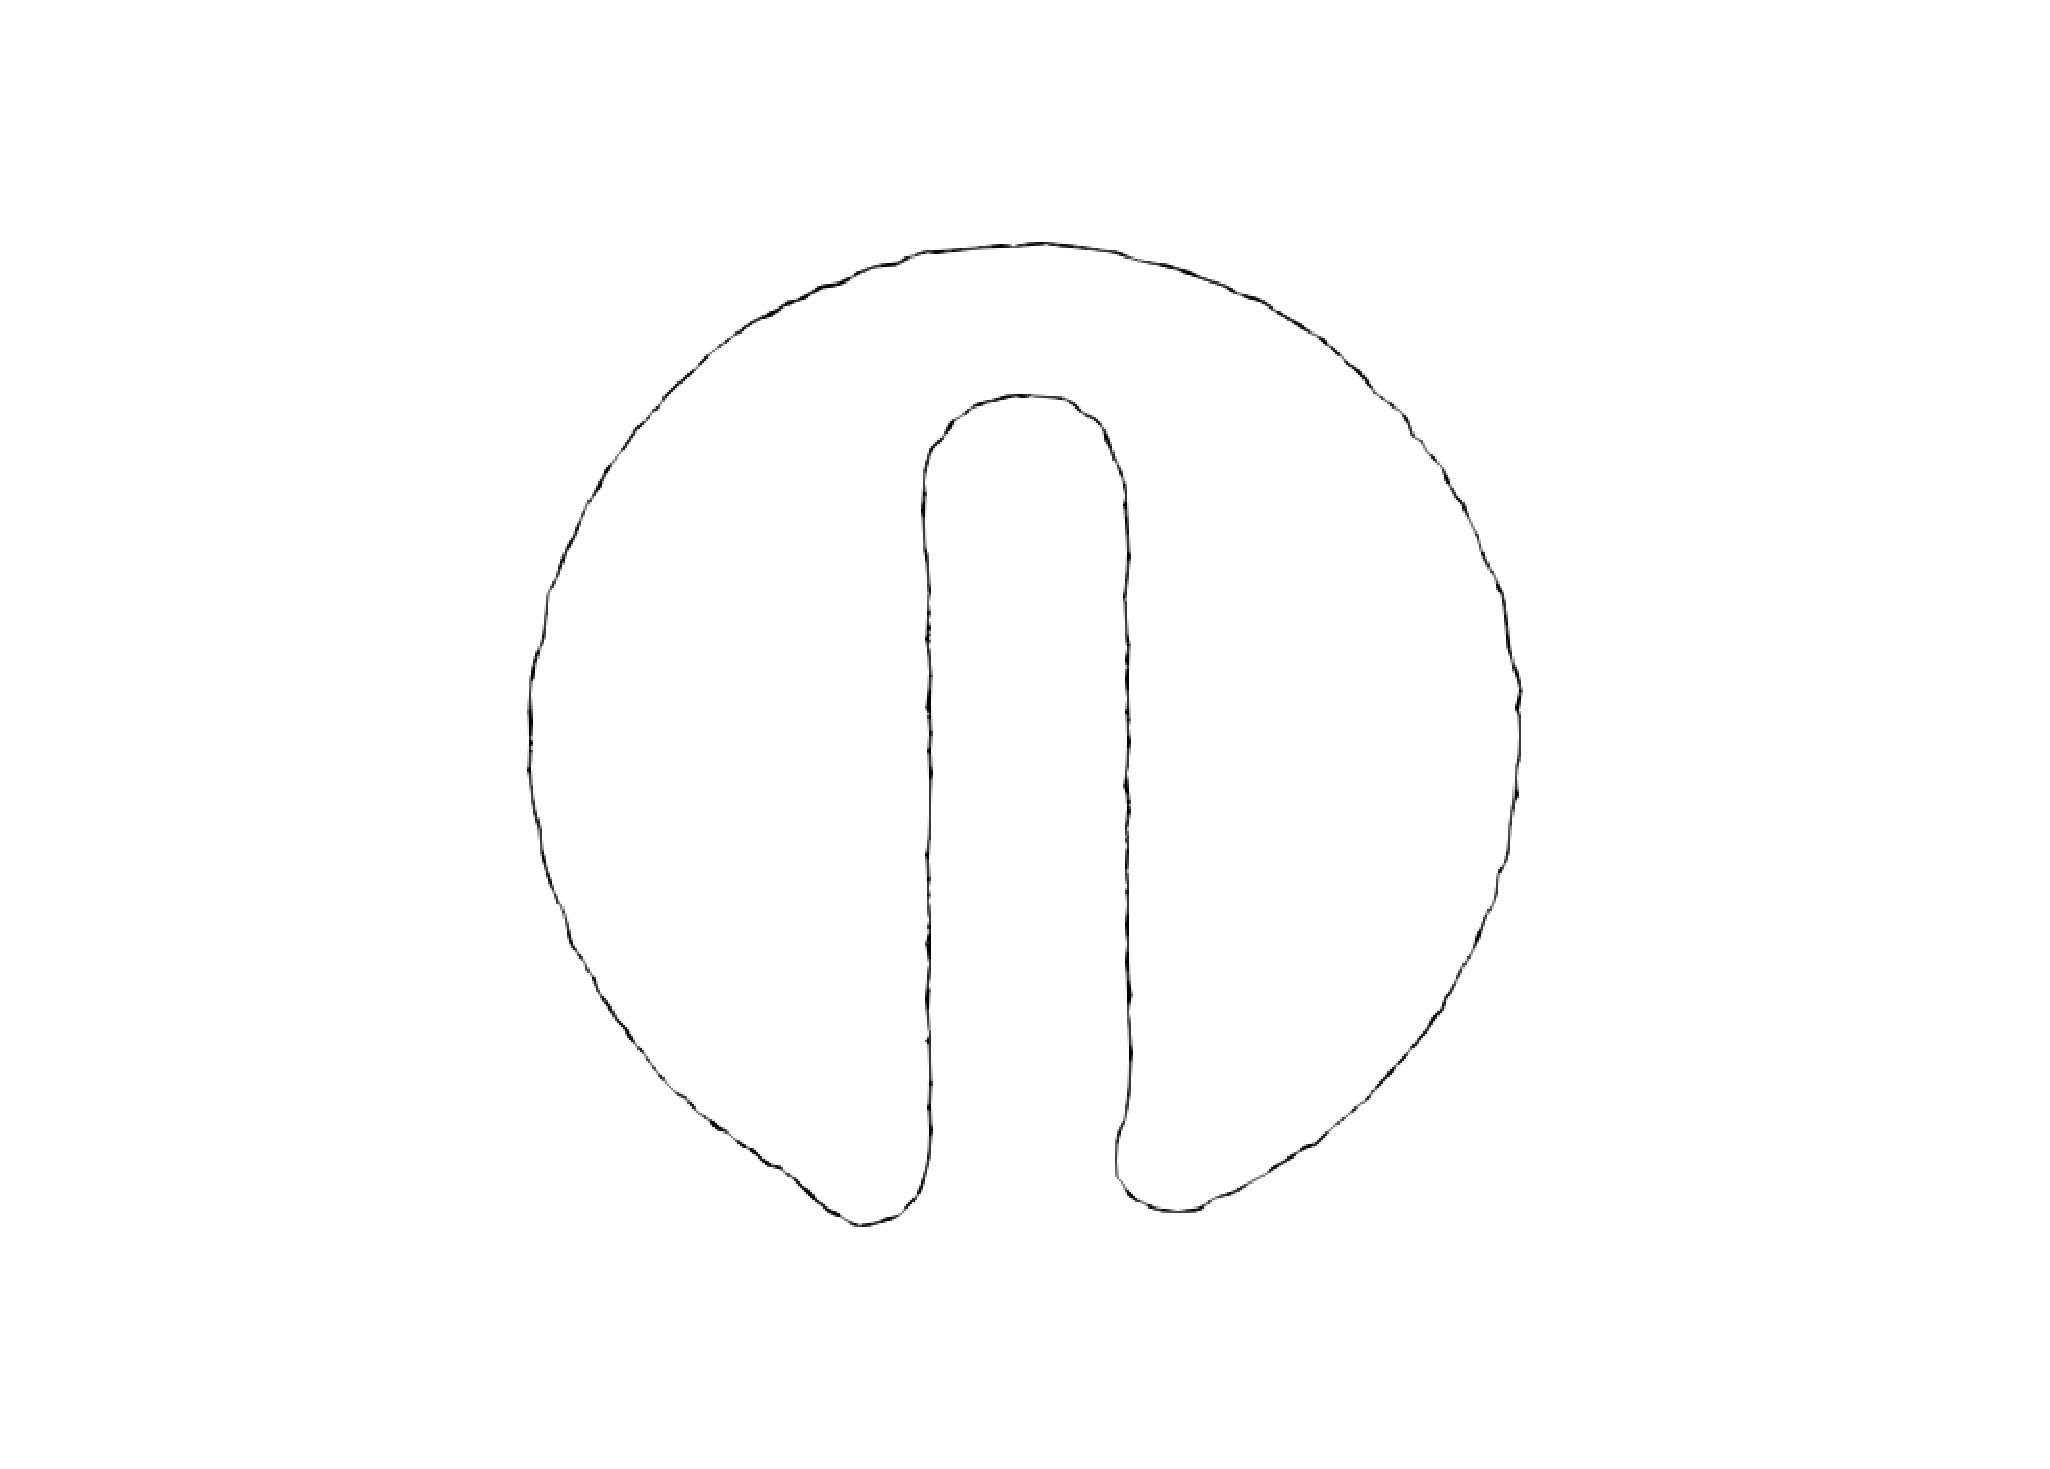
\includegraphics[width=0.3\textwidth]{ISOPolyCo05Mid.eps}
\label{fig:ISOPolyCo05Mid}
%\caption{fig2}
}
\caption{The shape after one circle with isoAdvector method:\subref{fig:ISOPolyCo01Coarse} 51967 and $Co=0.1$, \subref{fig:ISOPolyCo05Coarse} 51967 and $Co=0.5$,\subref{fig:ISOPolyCo05Mid} 203965 and $Co=0.5$}
\label{fig:ISOPoly}
\end{figure}
%%%%%%%%%%%%%%%%%%%%%%%%%%%%%%%%%%%%%%%%%%%%%%%%%%%%%%%%%
\begin{figure}[htbp]
\centering
\subfigure[]{
\centering
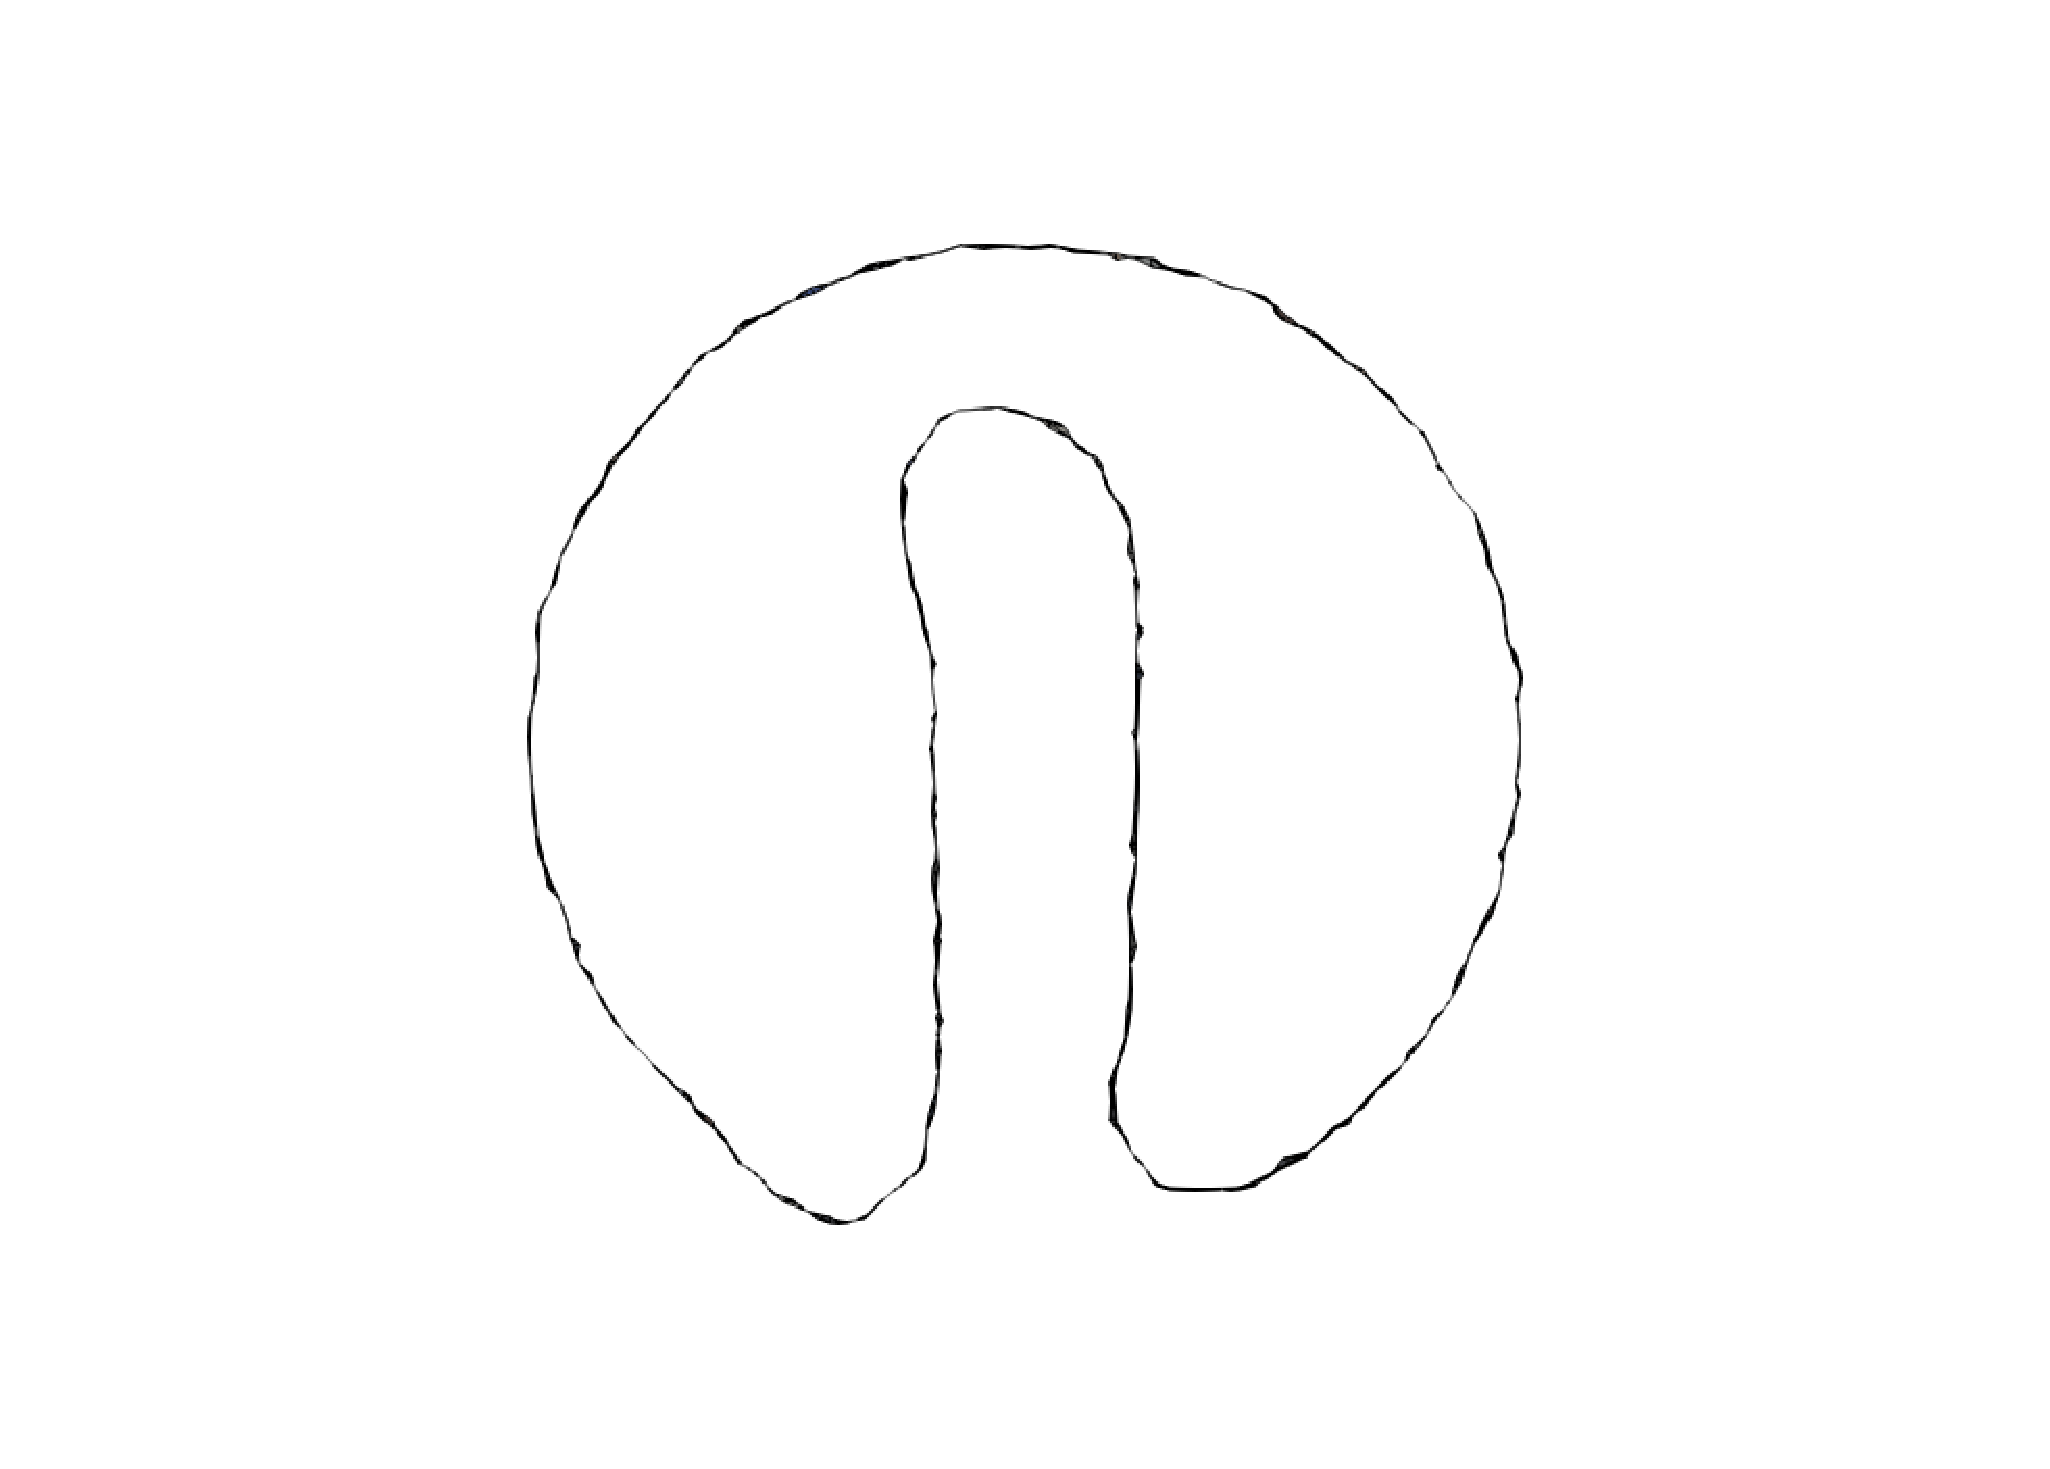
\includegraphics[width=0.3\textwidth]{CLSPolyCo01Coarse.eps}
%\caption{fig1}
\label{fig:CLSPolyCo01Coarse}
}
\subfigure[]{
\centering
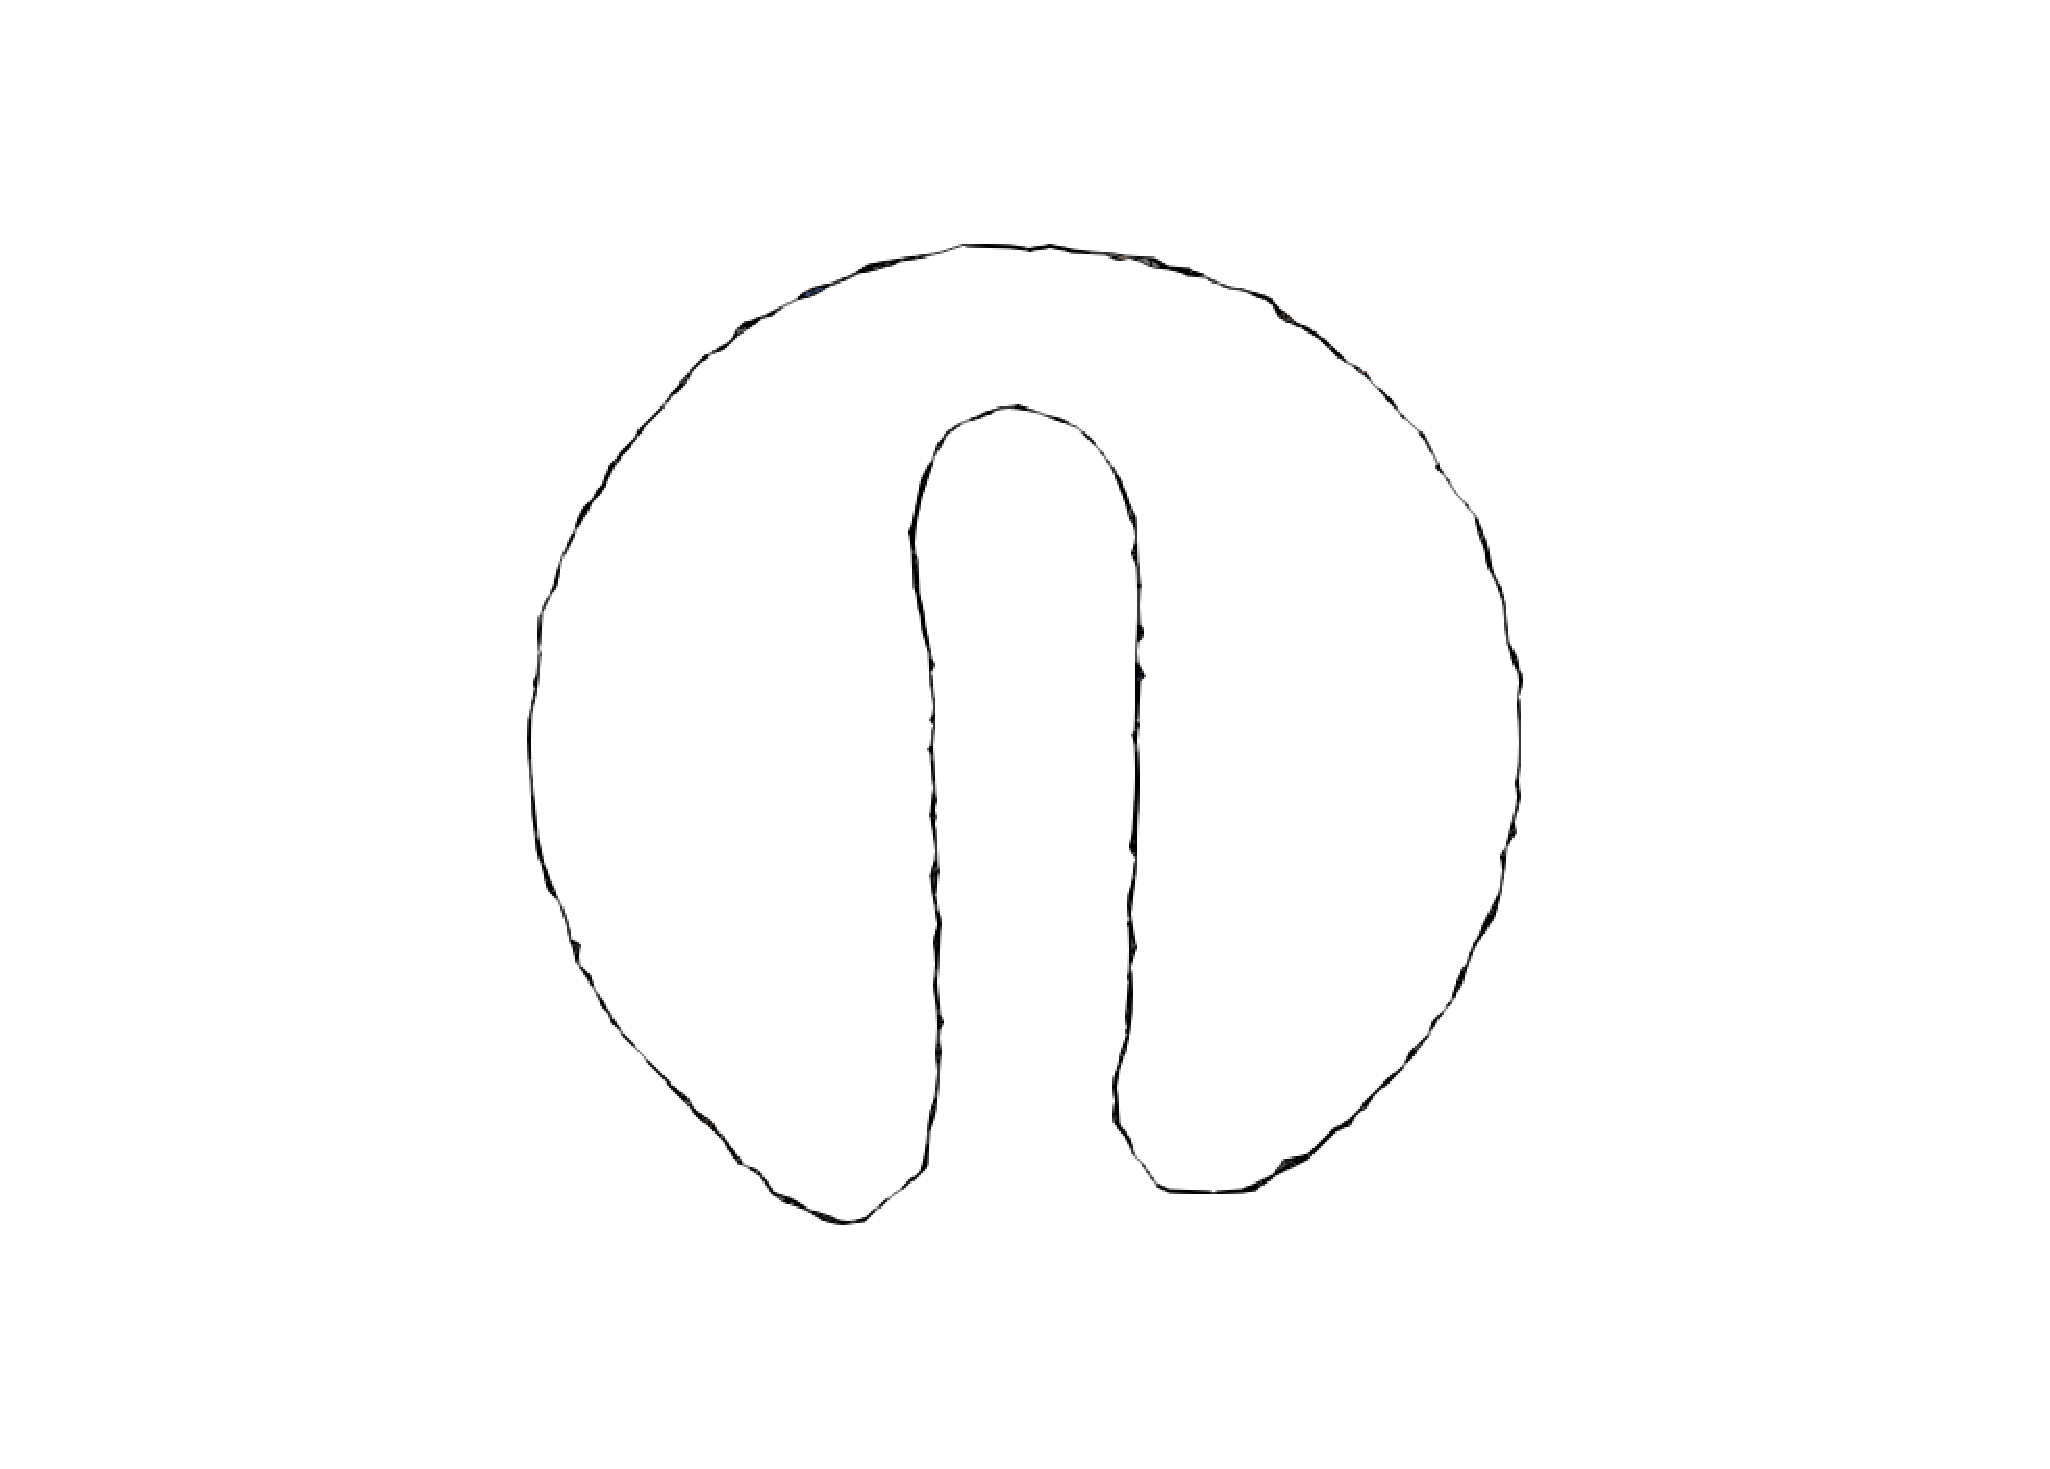
\includegraphics[width=0.3\textwidth]{CLSPolyCo05Coarse.eps}
%\caption{fig1}
\label{fig:CLSPolyCo05Coarse}
}
\subfigure[]{
\centering
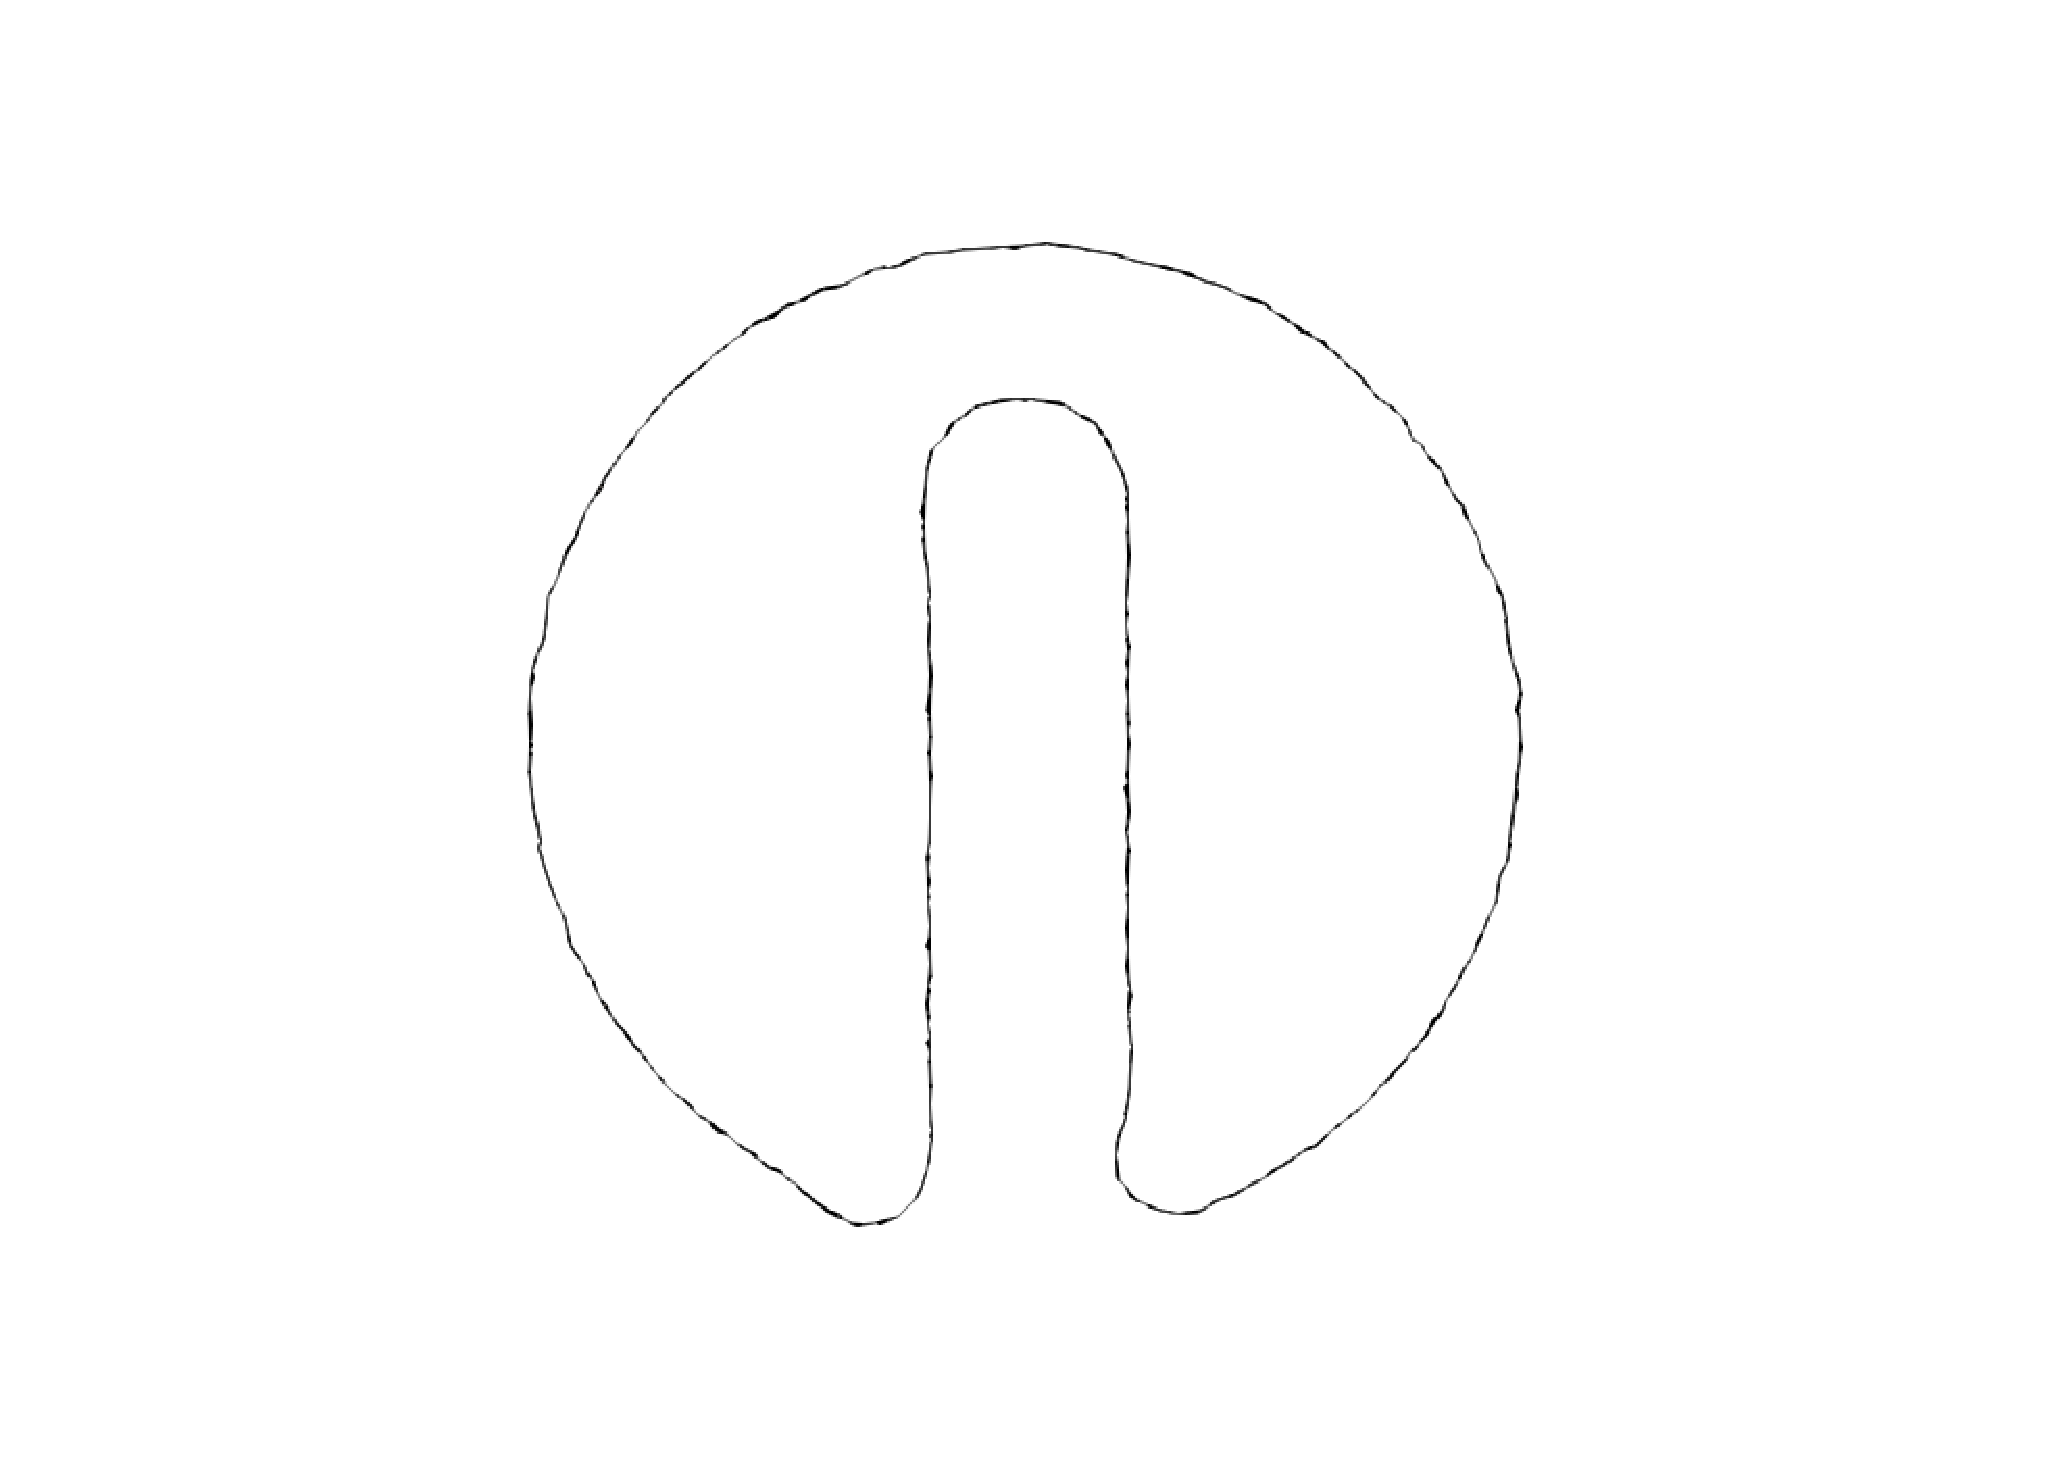
\includegraphics[width=0.3\textwidth]{CLSPolyCo05Mid.eps}
\label{fig:CLSPolyCo05Mid}
%\caption{fig2}
}
\caption{The shape after one circle with CLSAdvection:\subref{fig:CLSPolyCo01Coarse} 51967 and $Co=0.1$, \subref{fig:CLSPolyCo05Coarse} 51967 and $Co=0.5$,\subref{fig:CLSPolyCo05Mid} 203965 and $Co=0.5$}
\label{fig:CLSPoly}
\end{figure}
%%%%%%%%%%%%%%%%%%%%%%%%%%%%%%%%%%%%%%%%%%%%%%%%%%%%%%%%
\begin{figure}[htbp]
\centering
\subfigure[]{
\centering
\includegraphics[width=0.4\textwidth]{0_coarse_trio.eps}
%\caption{fig1}
\label{fig:trioCoarse}
}
\subfigure[]{
\centering
\includegraphics[width=0.4\textwidth]{0_mid_trio.eps}
\label{fig:trioMid}
%\caption{fig2}
}
\caption{Initial shape in triangle meshes with different cell numbers:\subref{fig:trioCoarse} 68805, \subref{fig:trioMid} 277605}
\label{fig:trio0}
\end{figure}
%%%%%%%%%%%%%%%%%%%%%%%%%%%%%%%%%%%%%%%%%%%%%%%%%%%%%%%
\begin{figure}[htbp]
\centering
\subfigure[]{
\centering
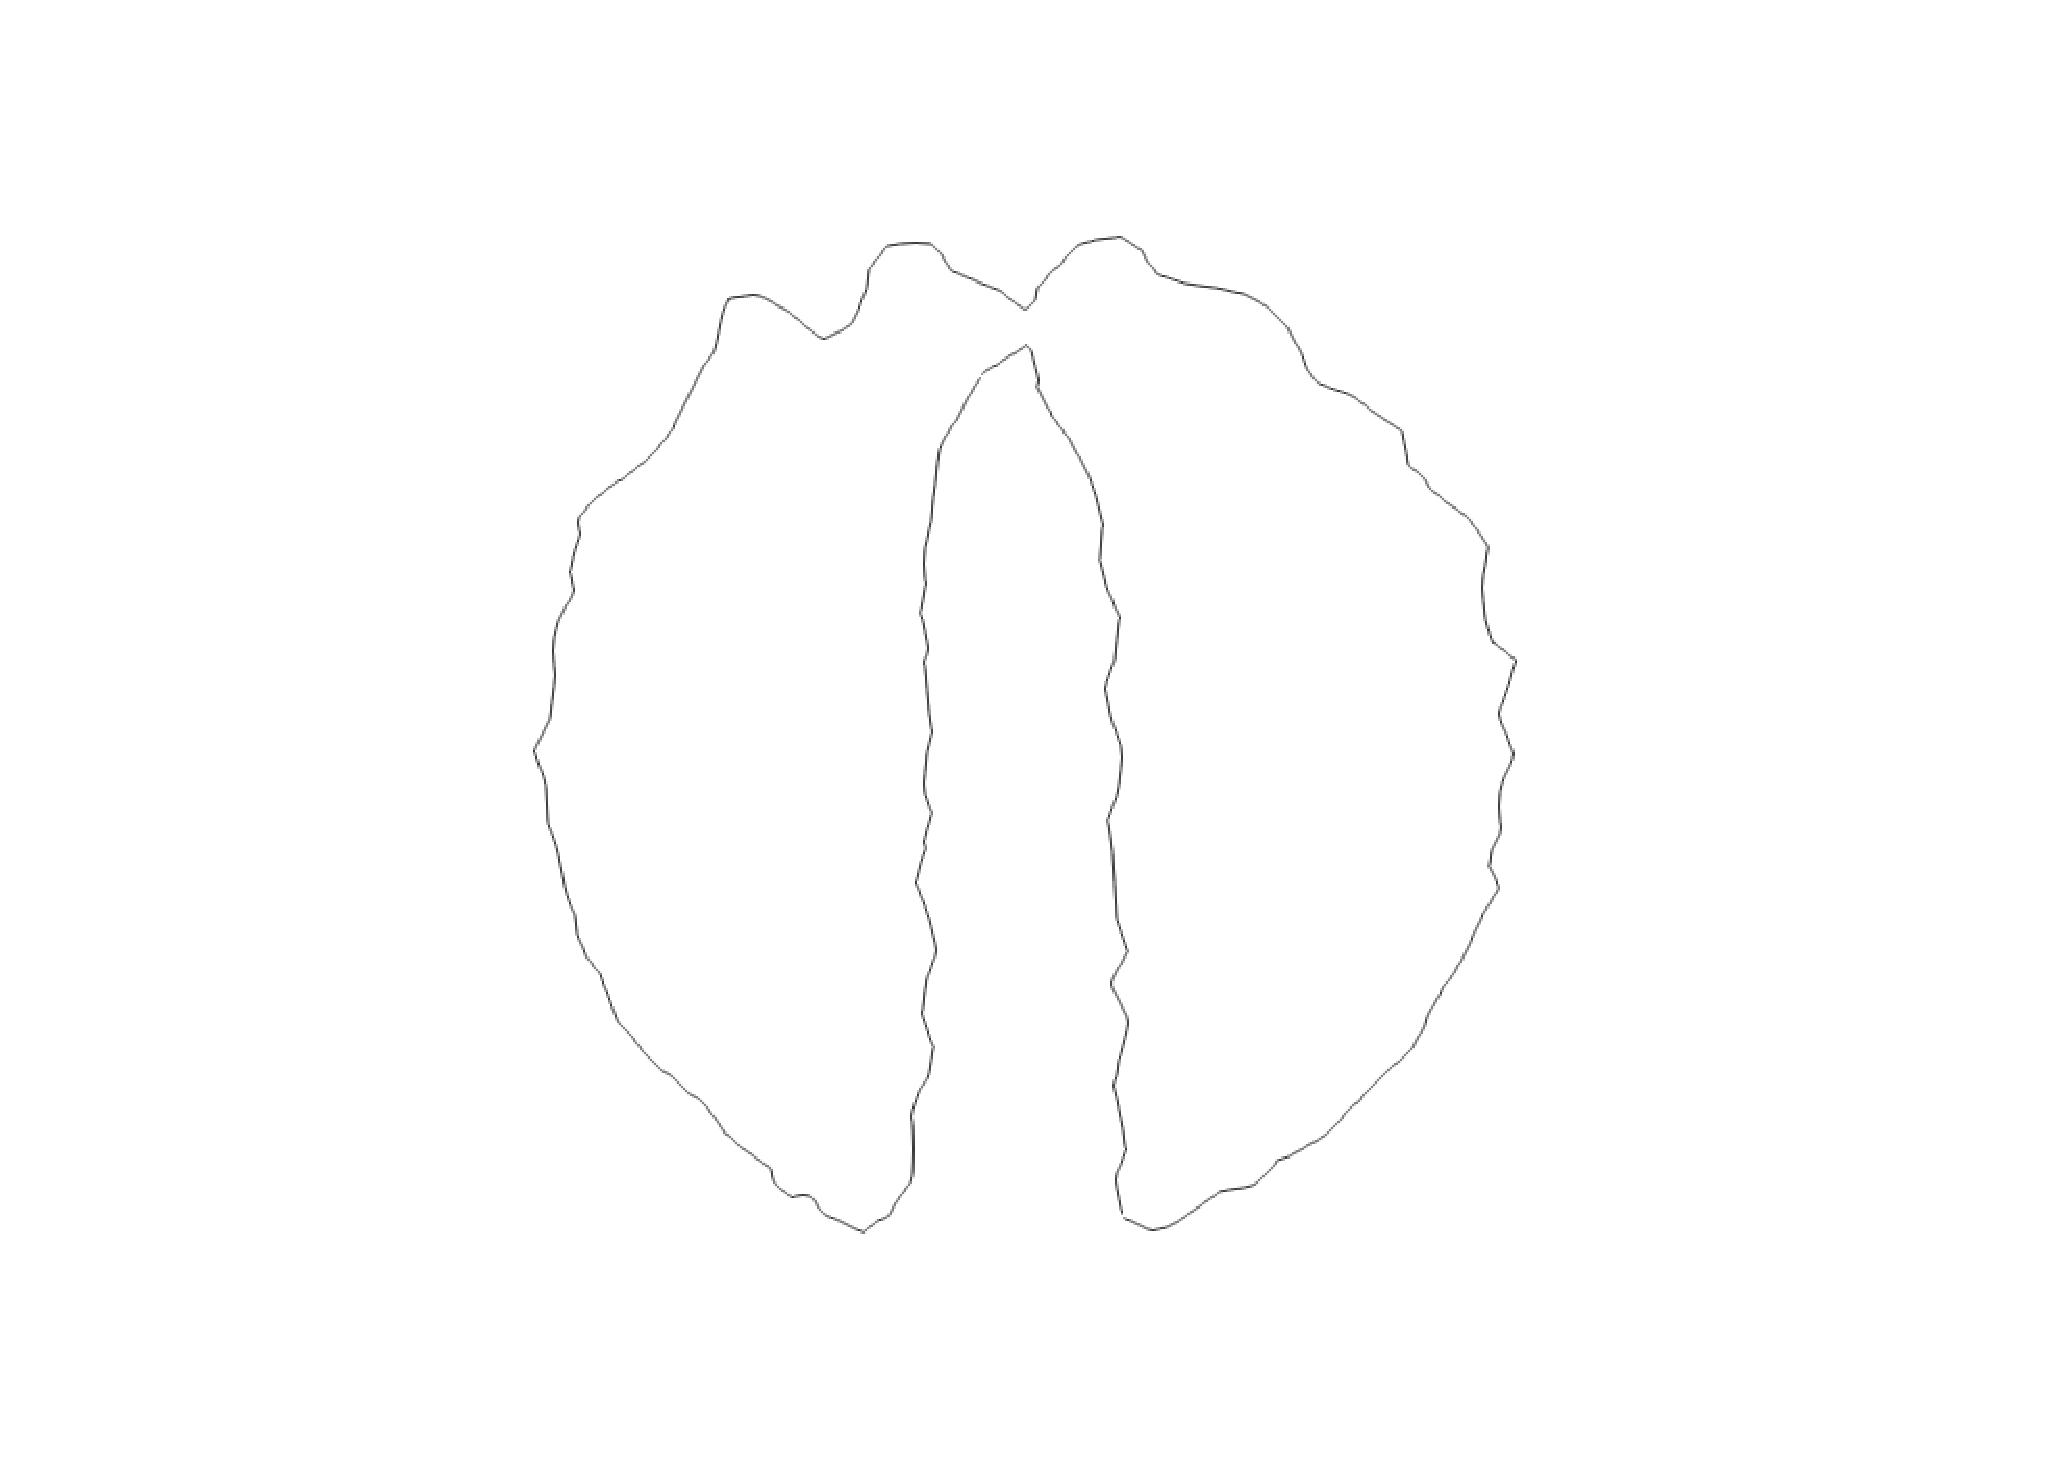
\includegraphics[width=0.3\textwidth]{MULESTriCo01Coarse.eps}
%\caption{fig1}
\label{fig:MULESTriCo01Coarse}
}
\subfigure[]{
\centering
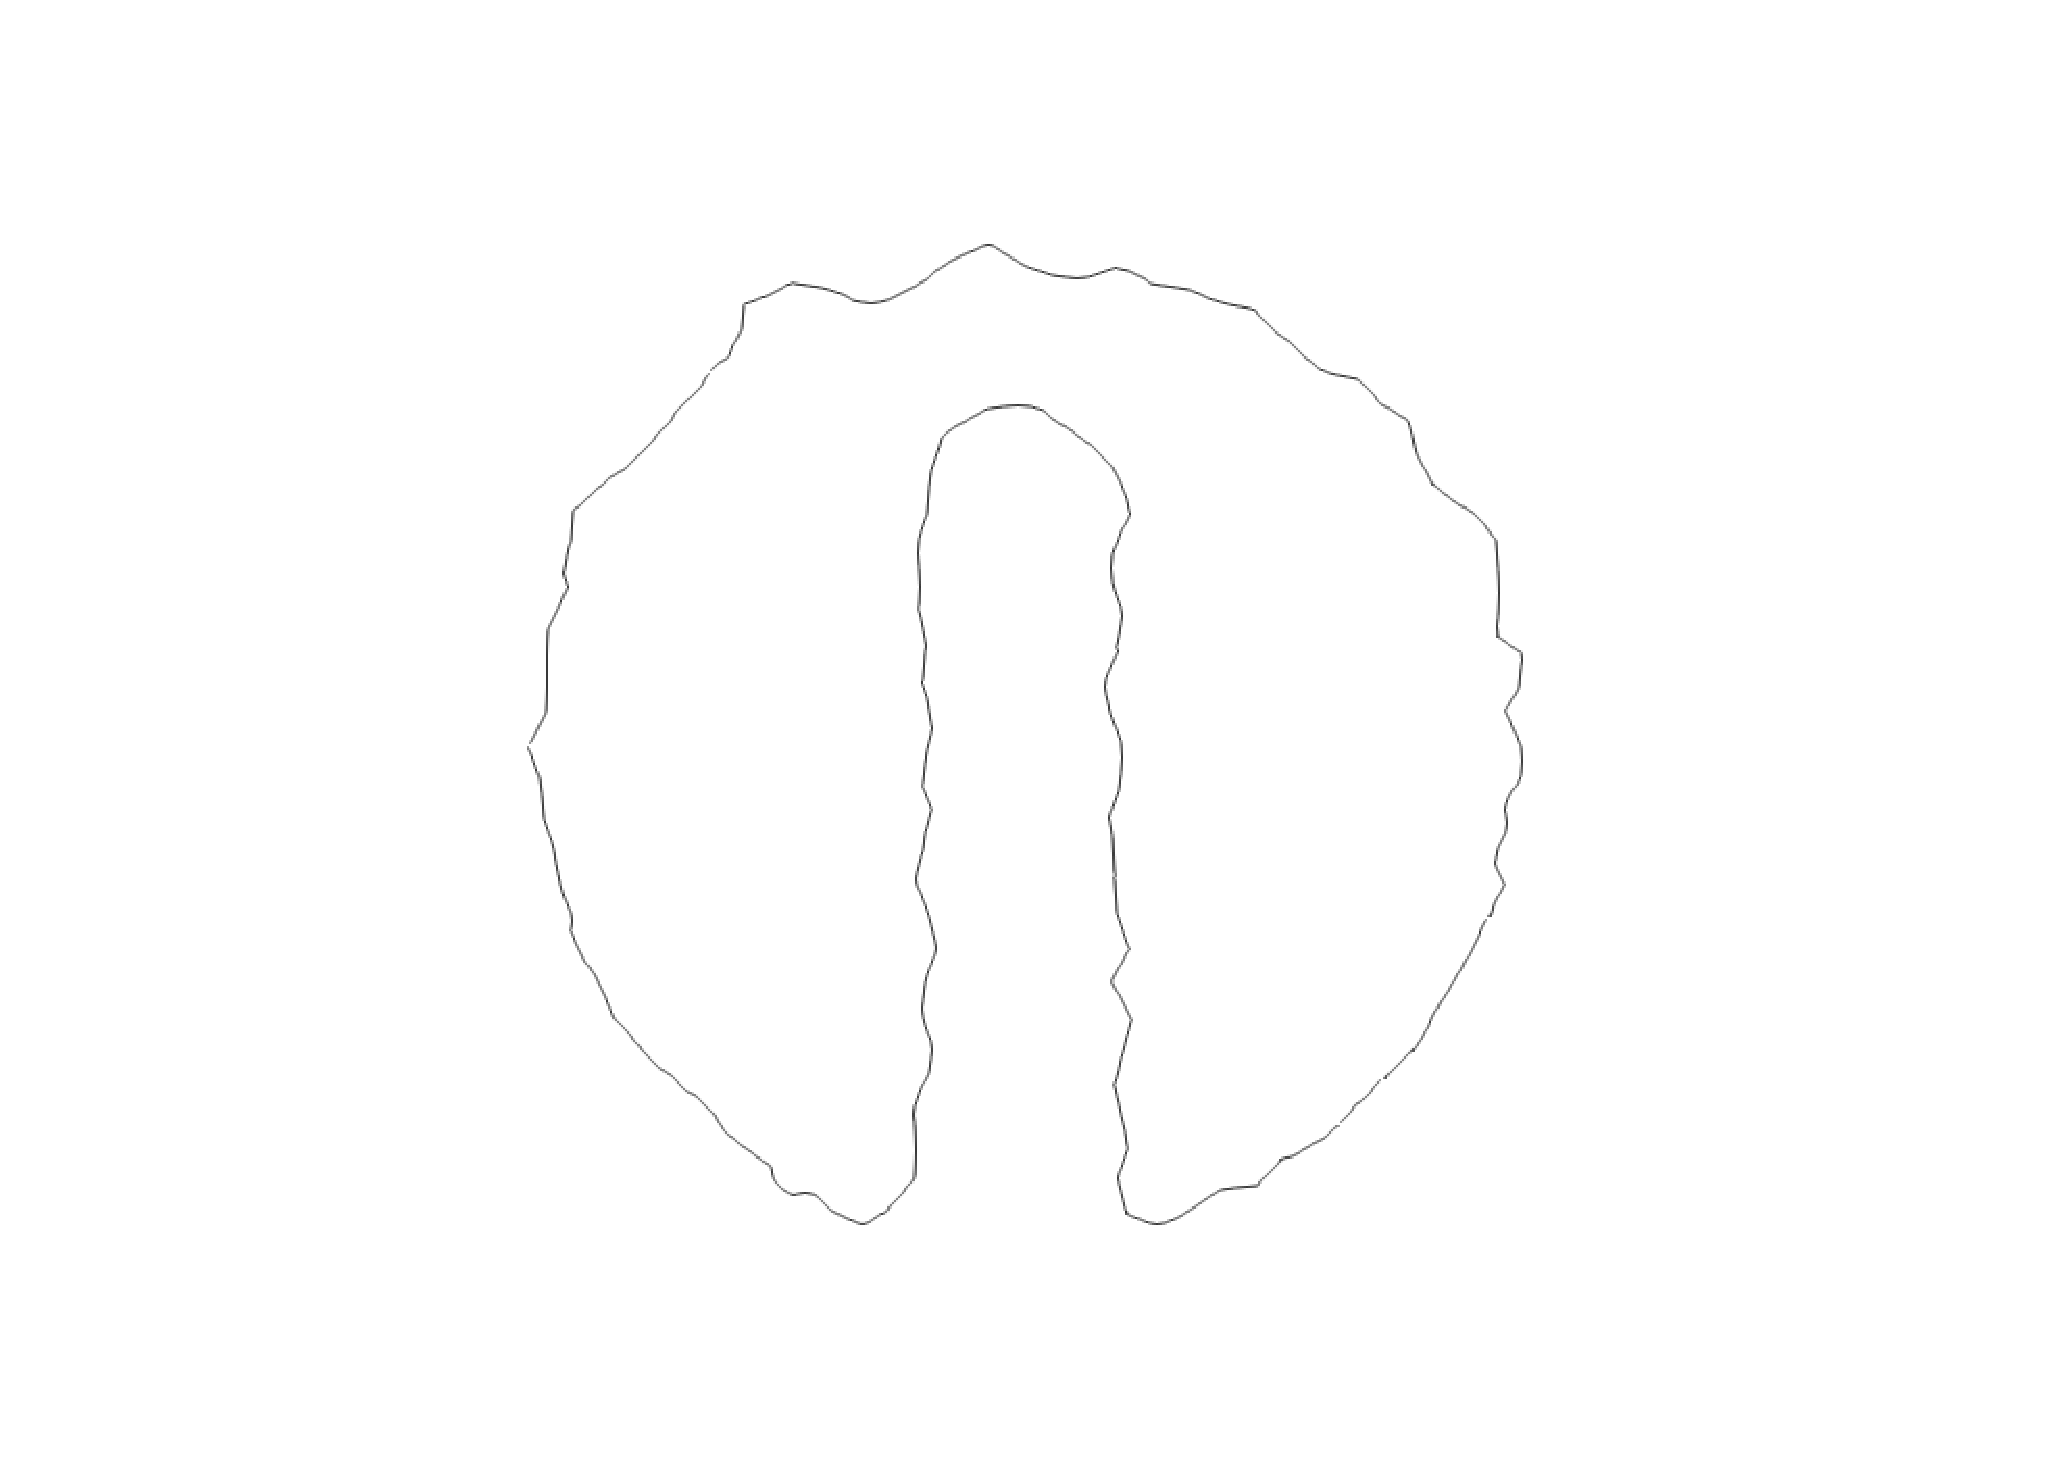
\includegraphics[width=0.3\textwidth]{MULESTriCo05Coarse.eps}
%\caption{fig1}
\label{fig:MULESTriCo05Coarse}
}
\subfigure[]{
\centering
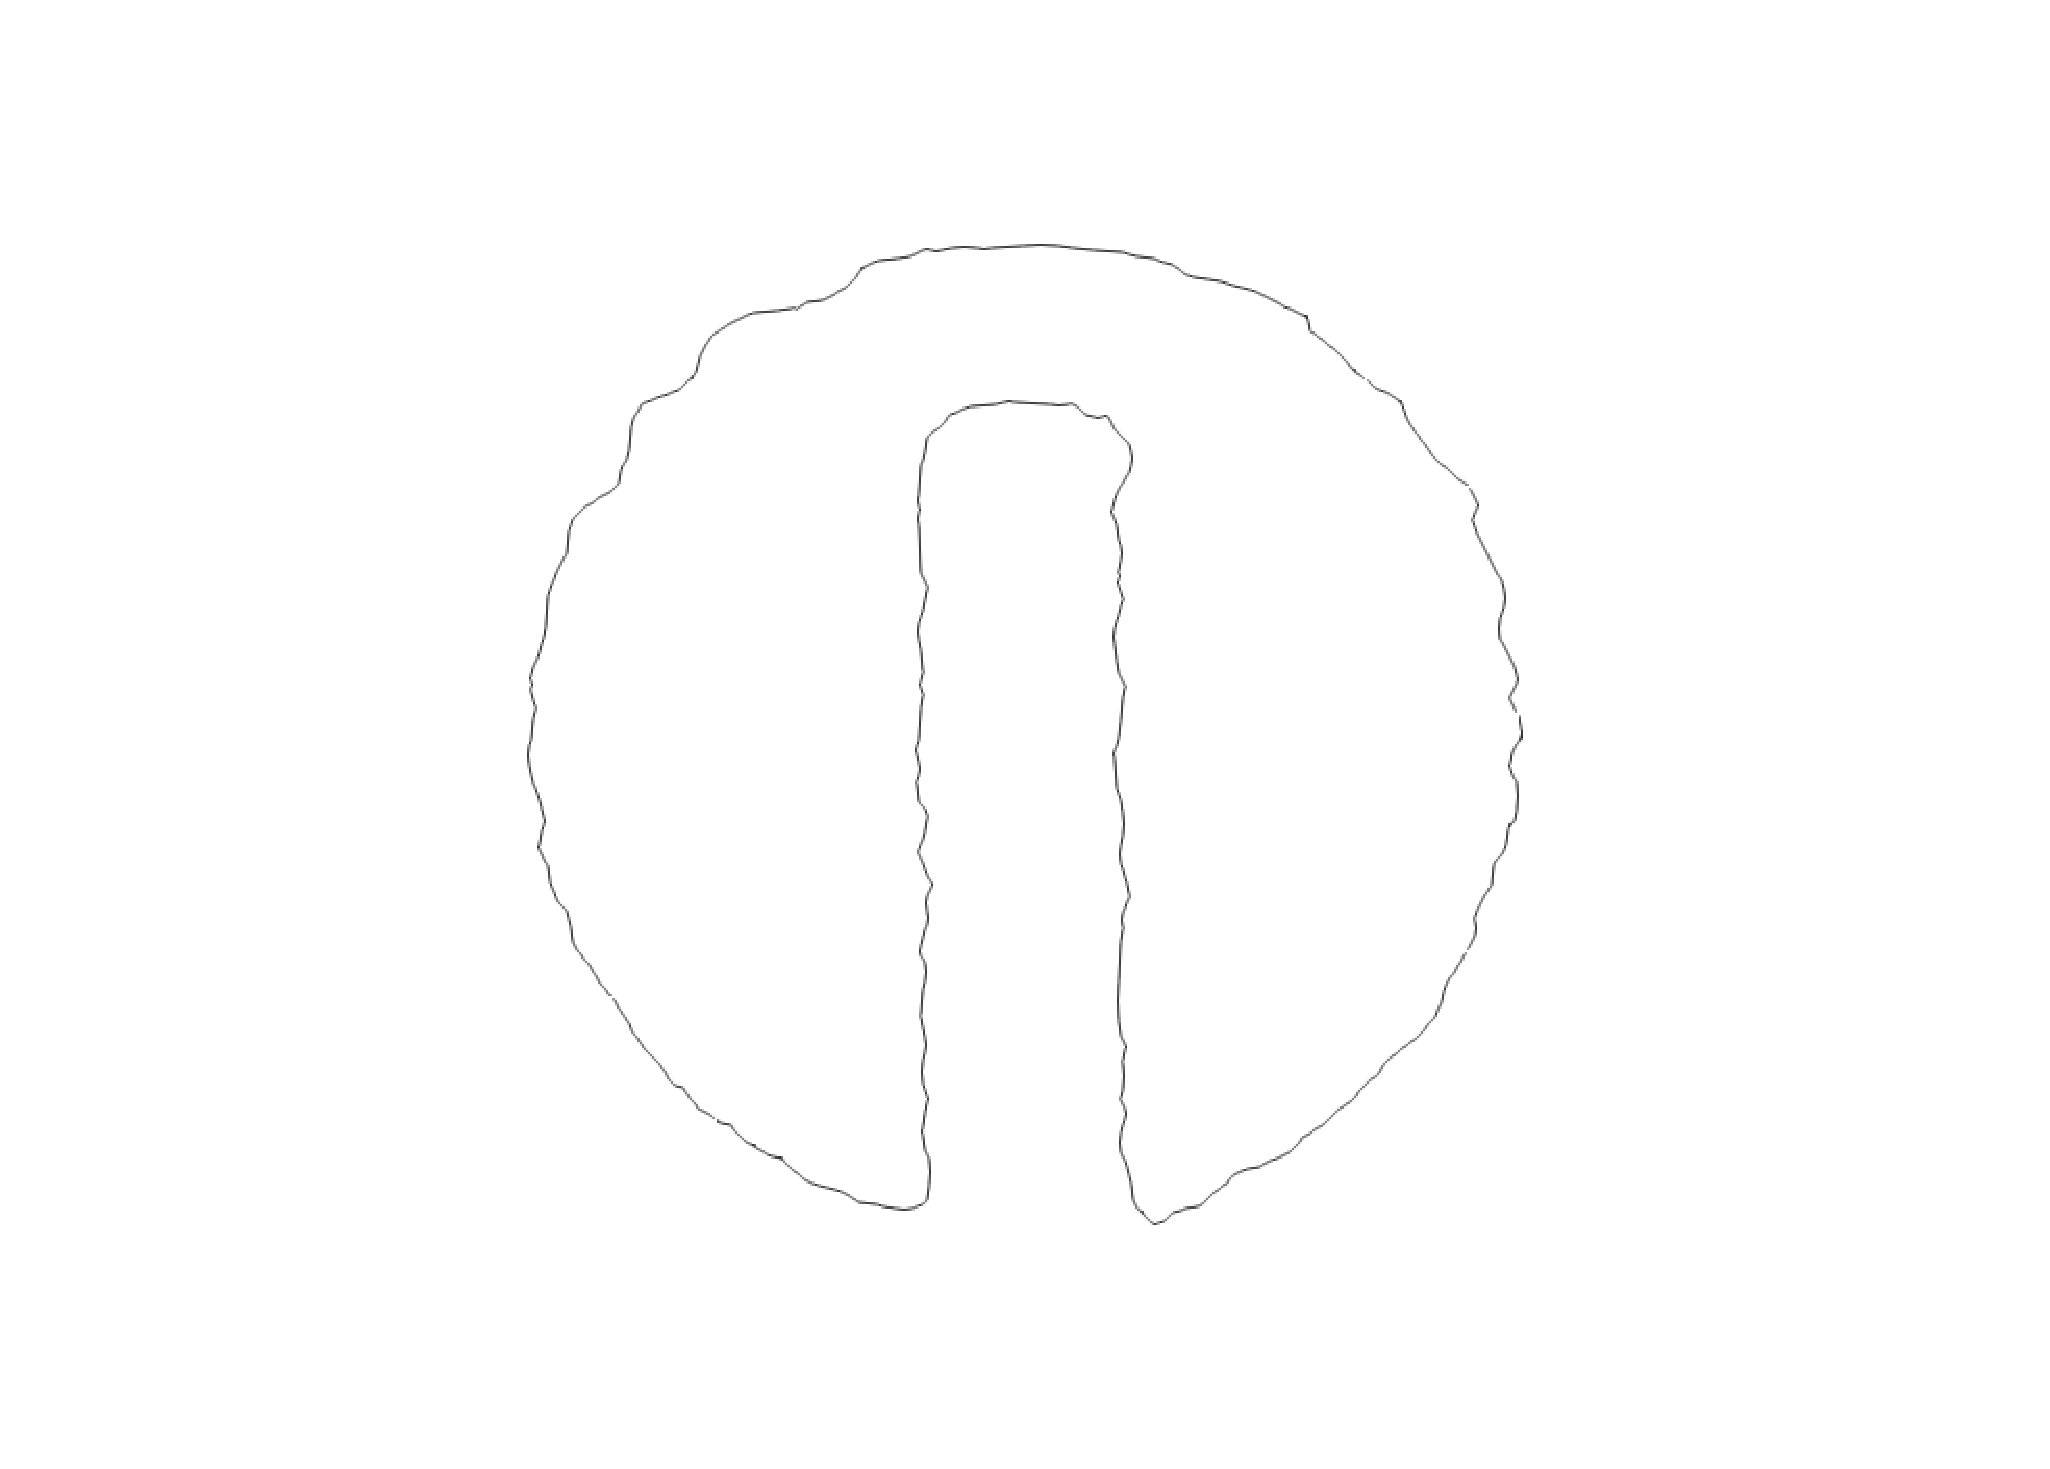
\includegraphics[width=0.3\textwidth]{MULESTriCo05Mid.eps}
\label{fig:MULESTriCo05Mid}
%\caption{fig2}
}
\caption{The shape after one circle with MULES method:\subref{fig:MULESTriCo01Coarse} 68805 and $Co=0.1$, \subref{fig:MULESTriCo05Coarse} 68805 and $Co=0.5$,\subref{fig:MULESTriCo05Mid} 203965 and $Co=0.5$}
\label{fig:MULESTri}
\end{figure}
%%%%%%%%%%%%%%%%%%%%%%%%%%%%%%%%%%%%%%%%%%%%%%%%%%%%%%
\begin{figure}[htbp]
\centering
\subfigure[]{
\centering
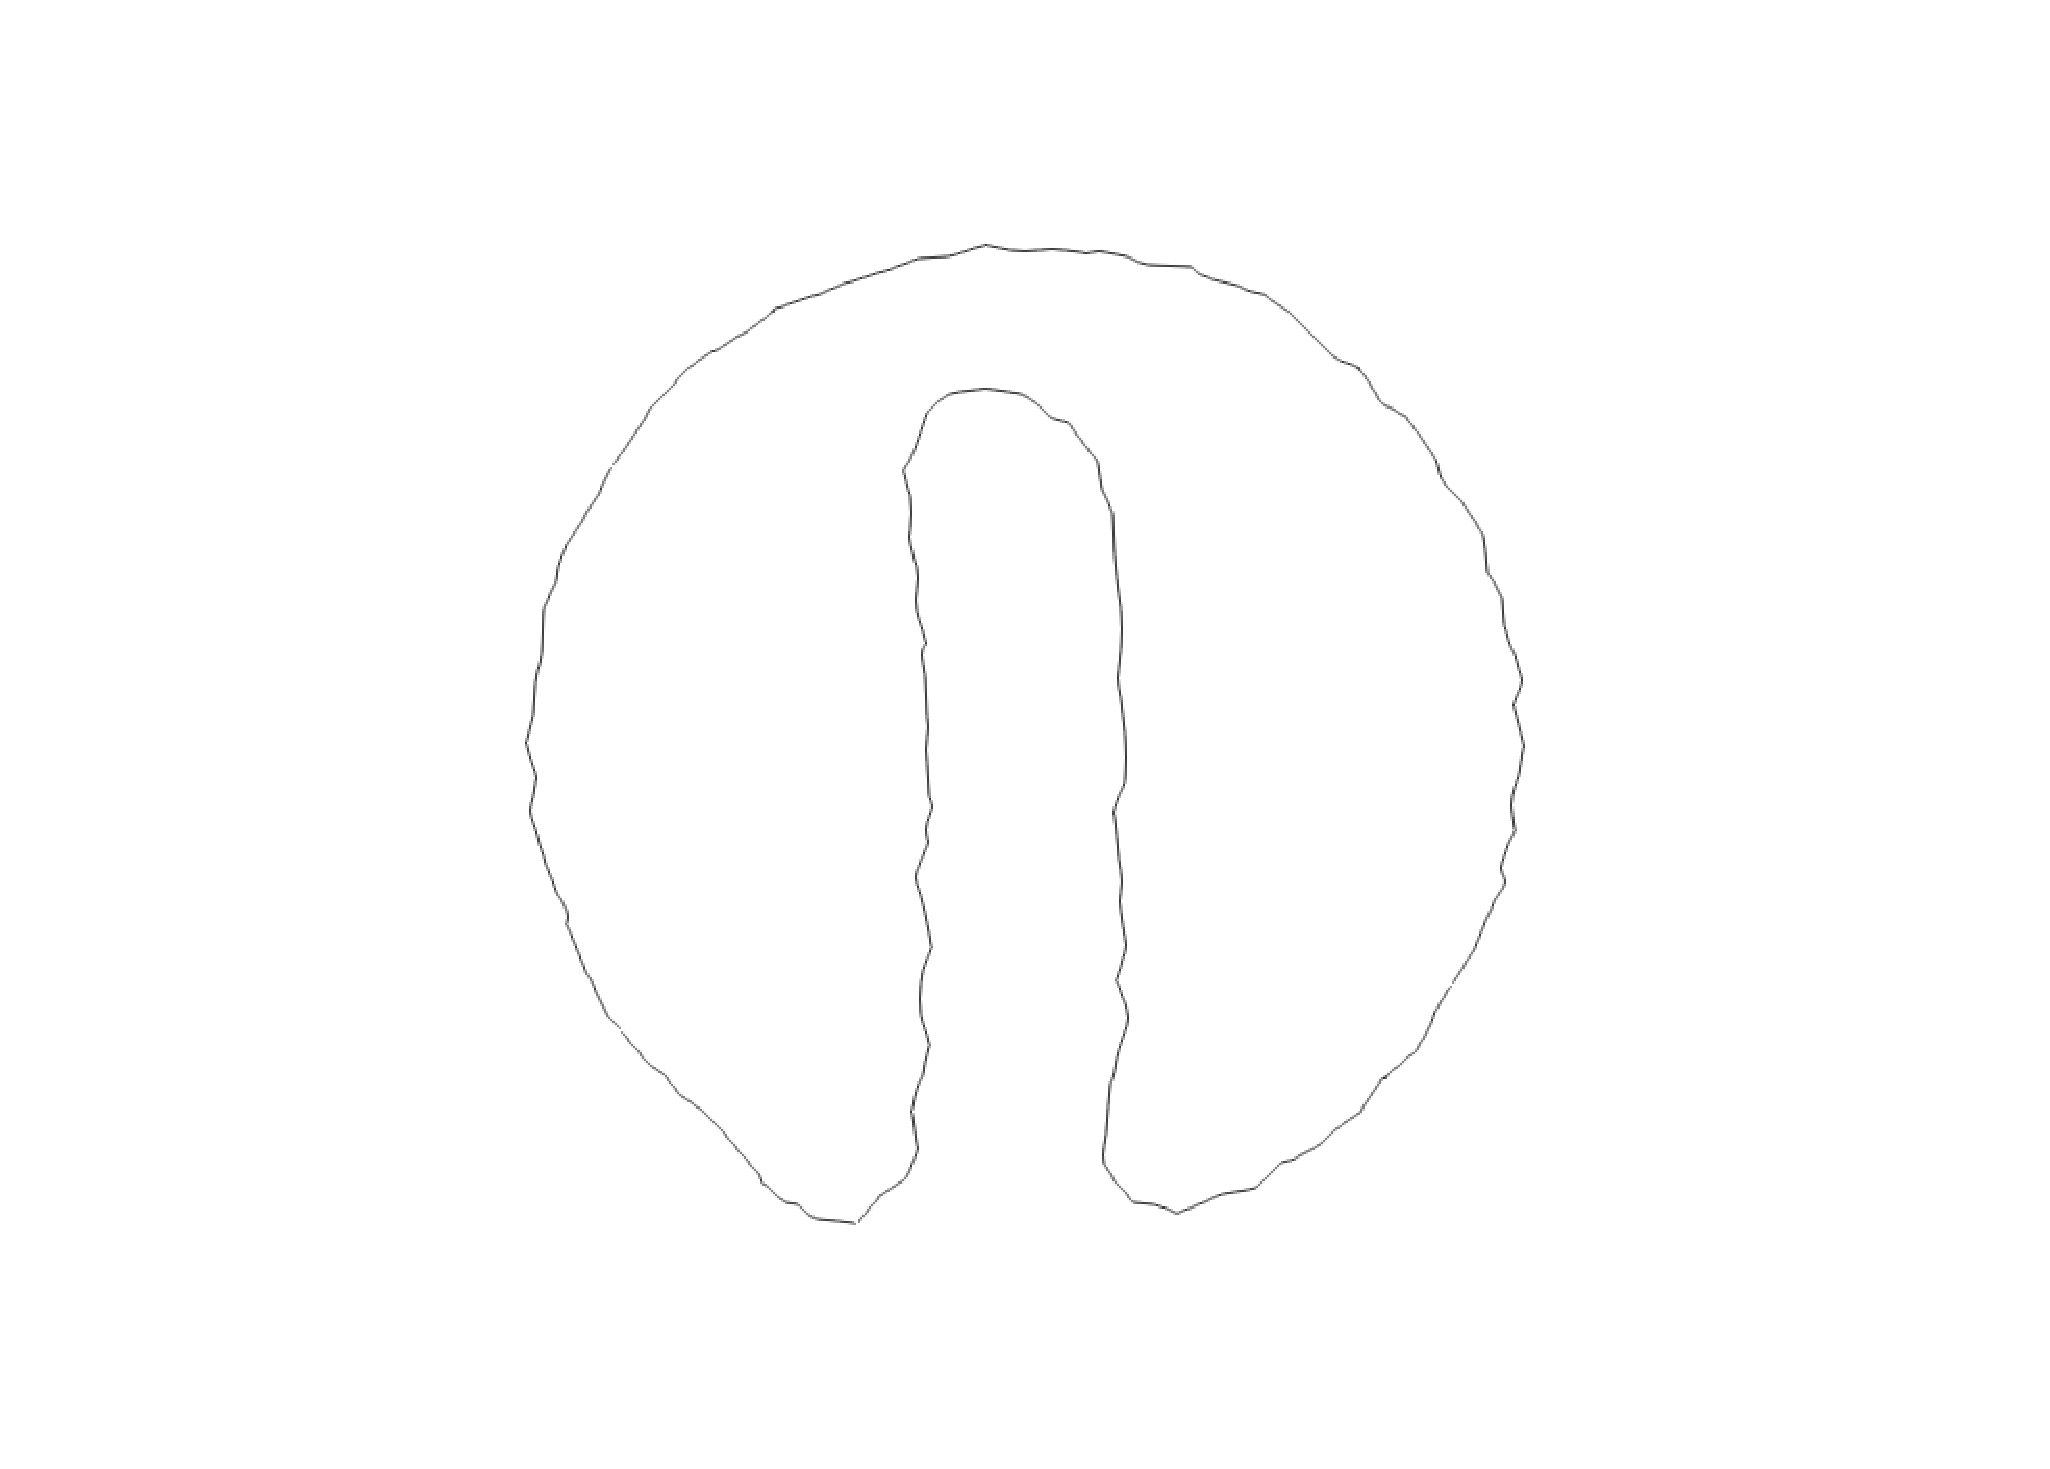
\includegraphics[width=0.3\textwidth]{ISOTriCo01Coarse.eps}
%\caption{fig1}
\label{fig:ISOTriCo01Coarse}
}
\subfigure[]{
\centering
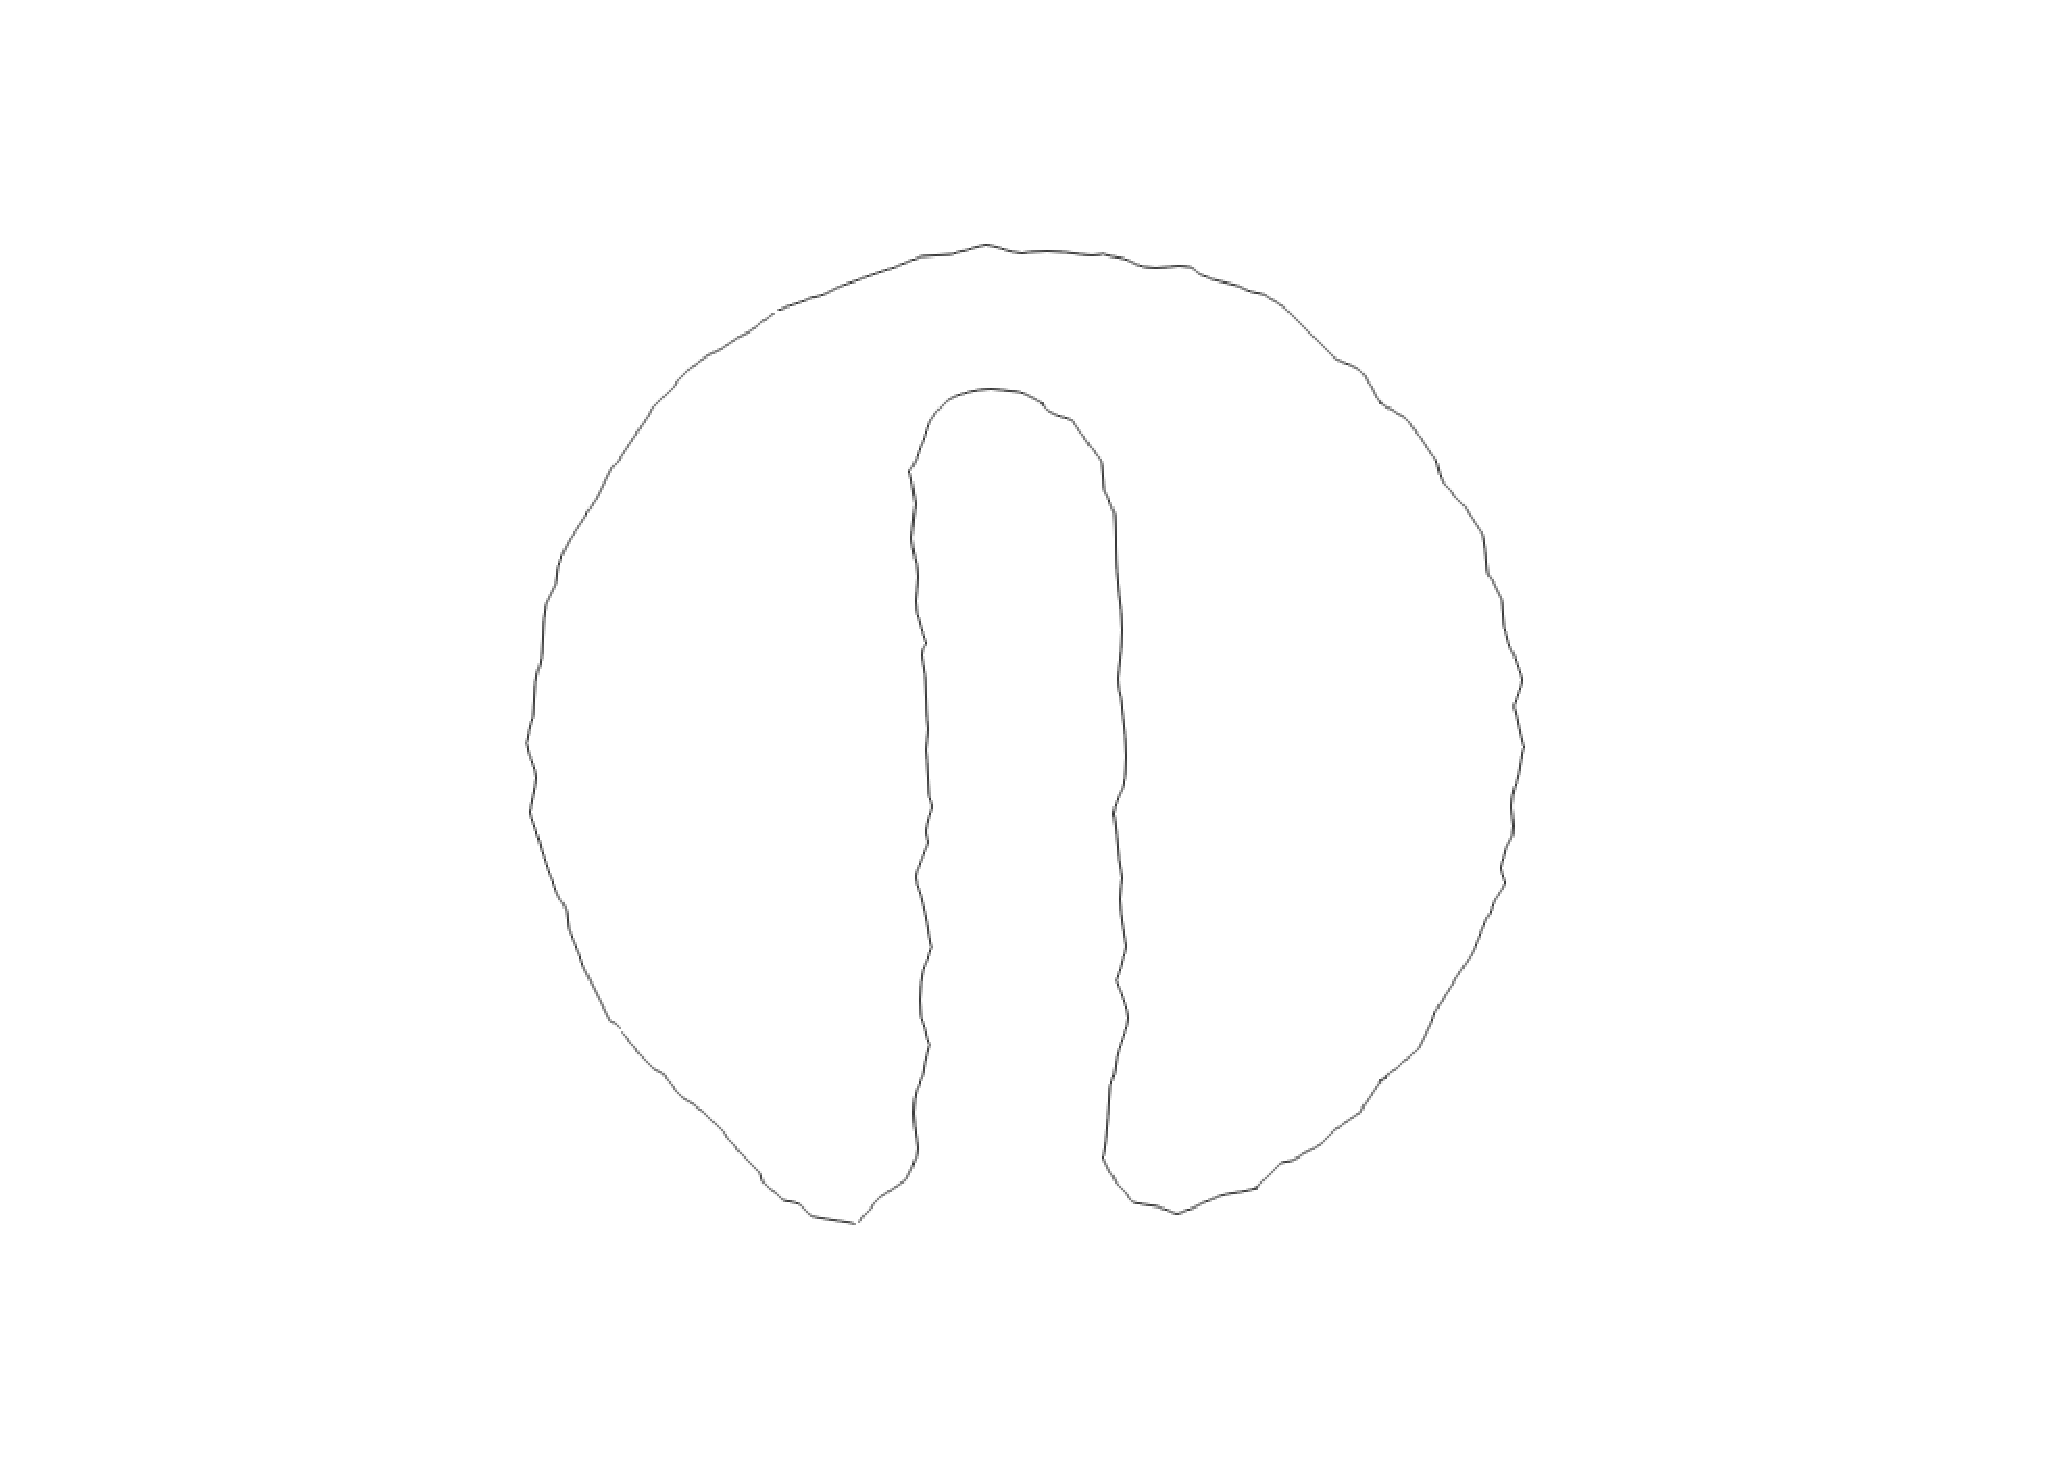
\includegraphics[width=0.3\textwidth]{ISOTriCo05Coarse.eps}
%\caption{fig1}
\label{fig:ISOTriCo05Coarse}
}
\subfigure[]{
\centering
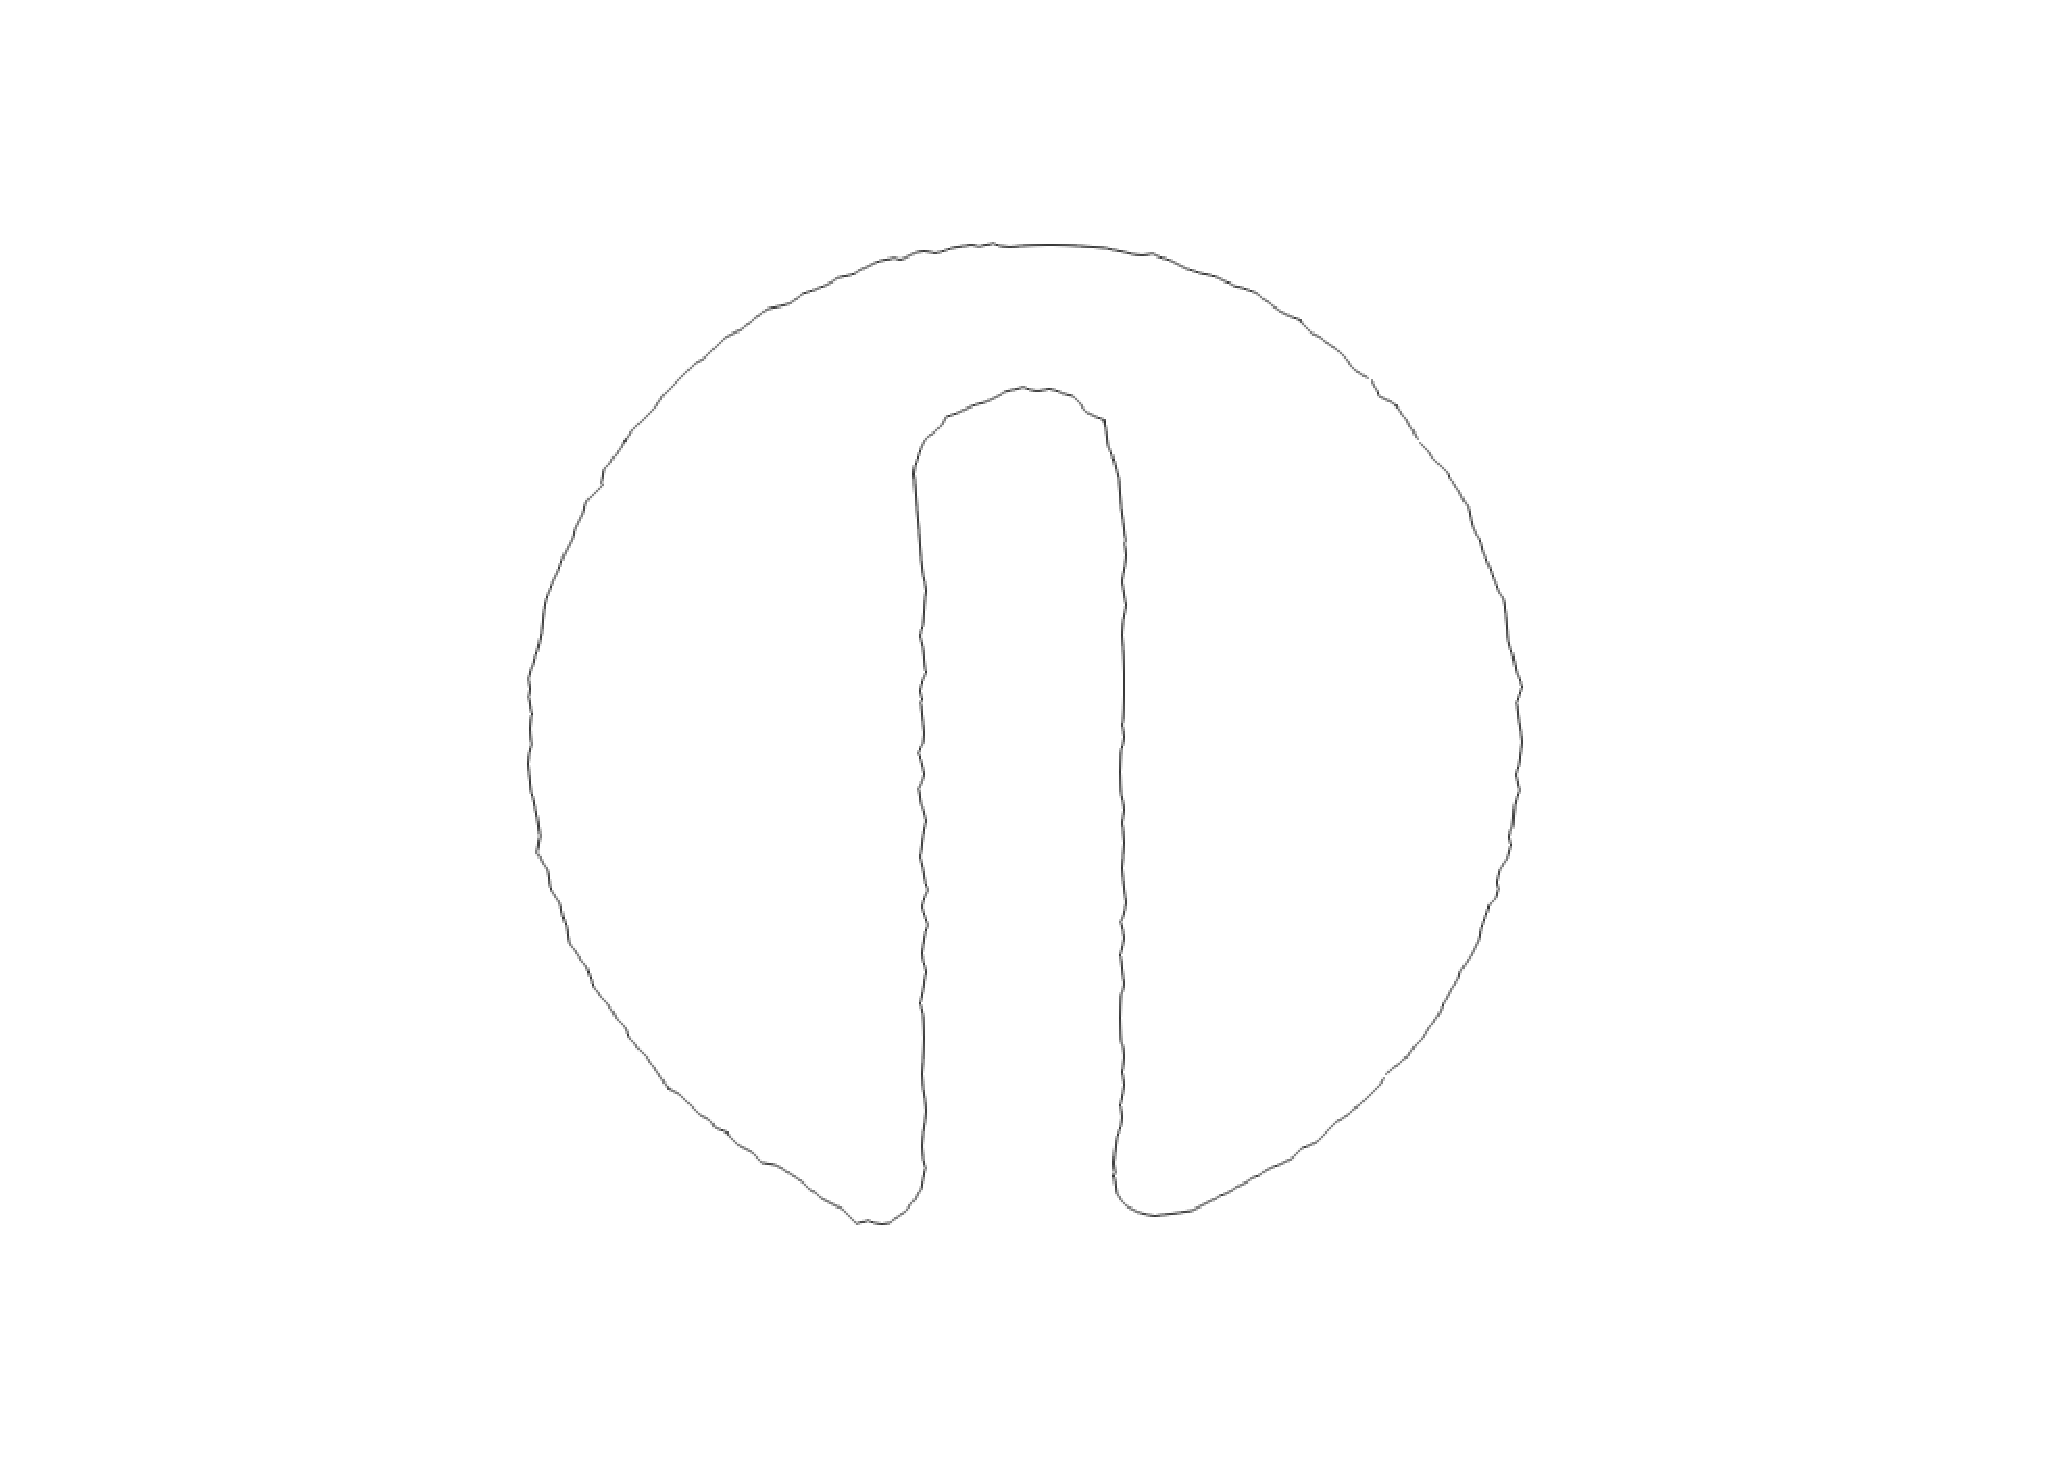
\includegraphics[width=0.3\textwidth]{ISOTriCo05Mid.eps}
\label{fig:ISOTriCo05Mid}
%\caption{fig2}
}
\caption{The shape after one circle with isoAdvector method:\subref{fig:ISOTriCo01Coarse} 68805 and $Co=0.1$, \subref{fig:ISOTriCo05Coarse} 68805 and $Co=0.5$,\subref{fig:ISOTriCo05Mid} 203965 and $Co=0.5$}
\label{fig:ISOTri}
\end{figure}
%%%%%%%%%%%%%%%%%%%%%%%%%%%%%%%%%%%%%%%%%%%%%%%%%%%%%
\begin{figure}[htbp]
\centering
\subfigure[]{
\centering
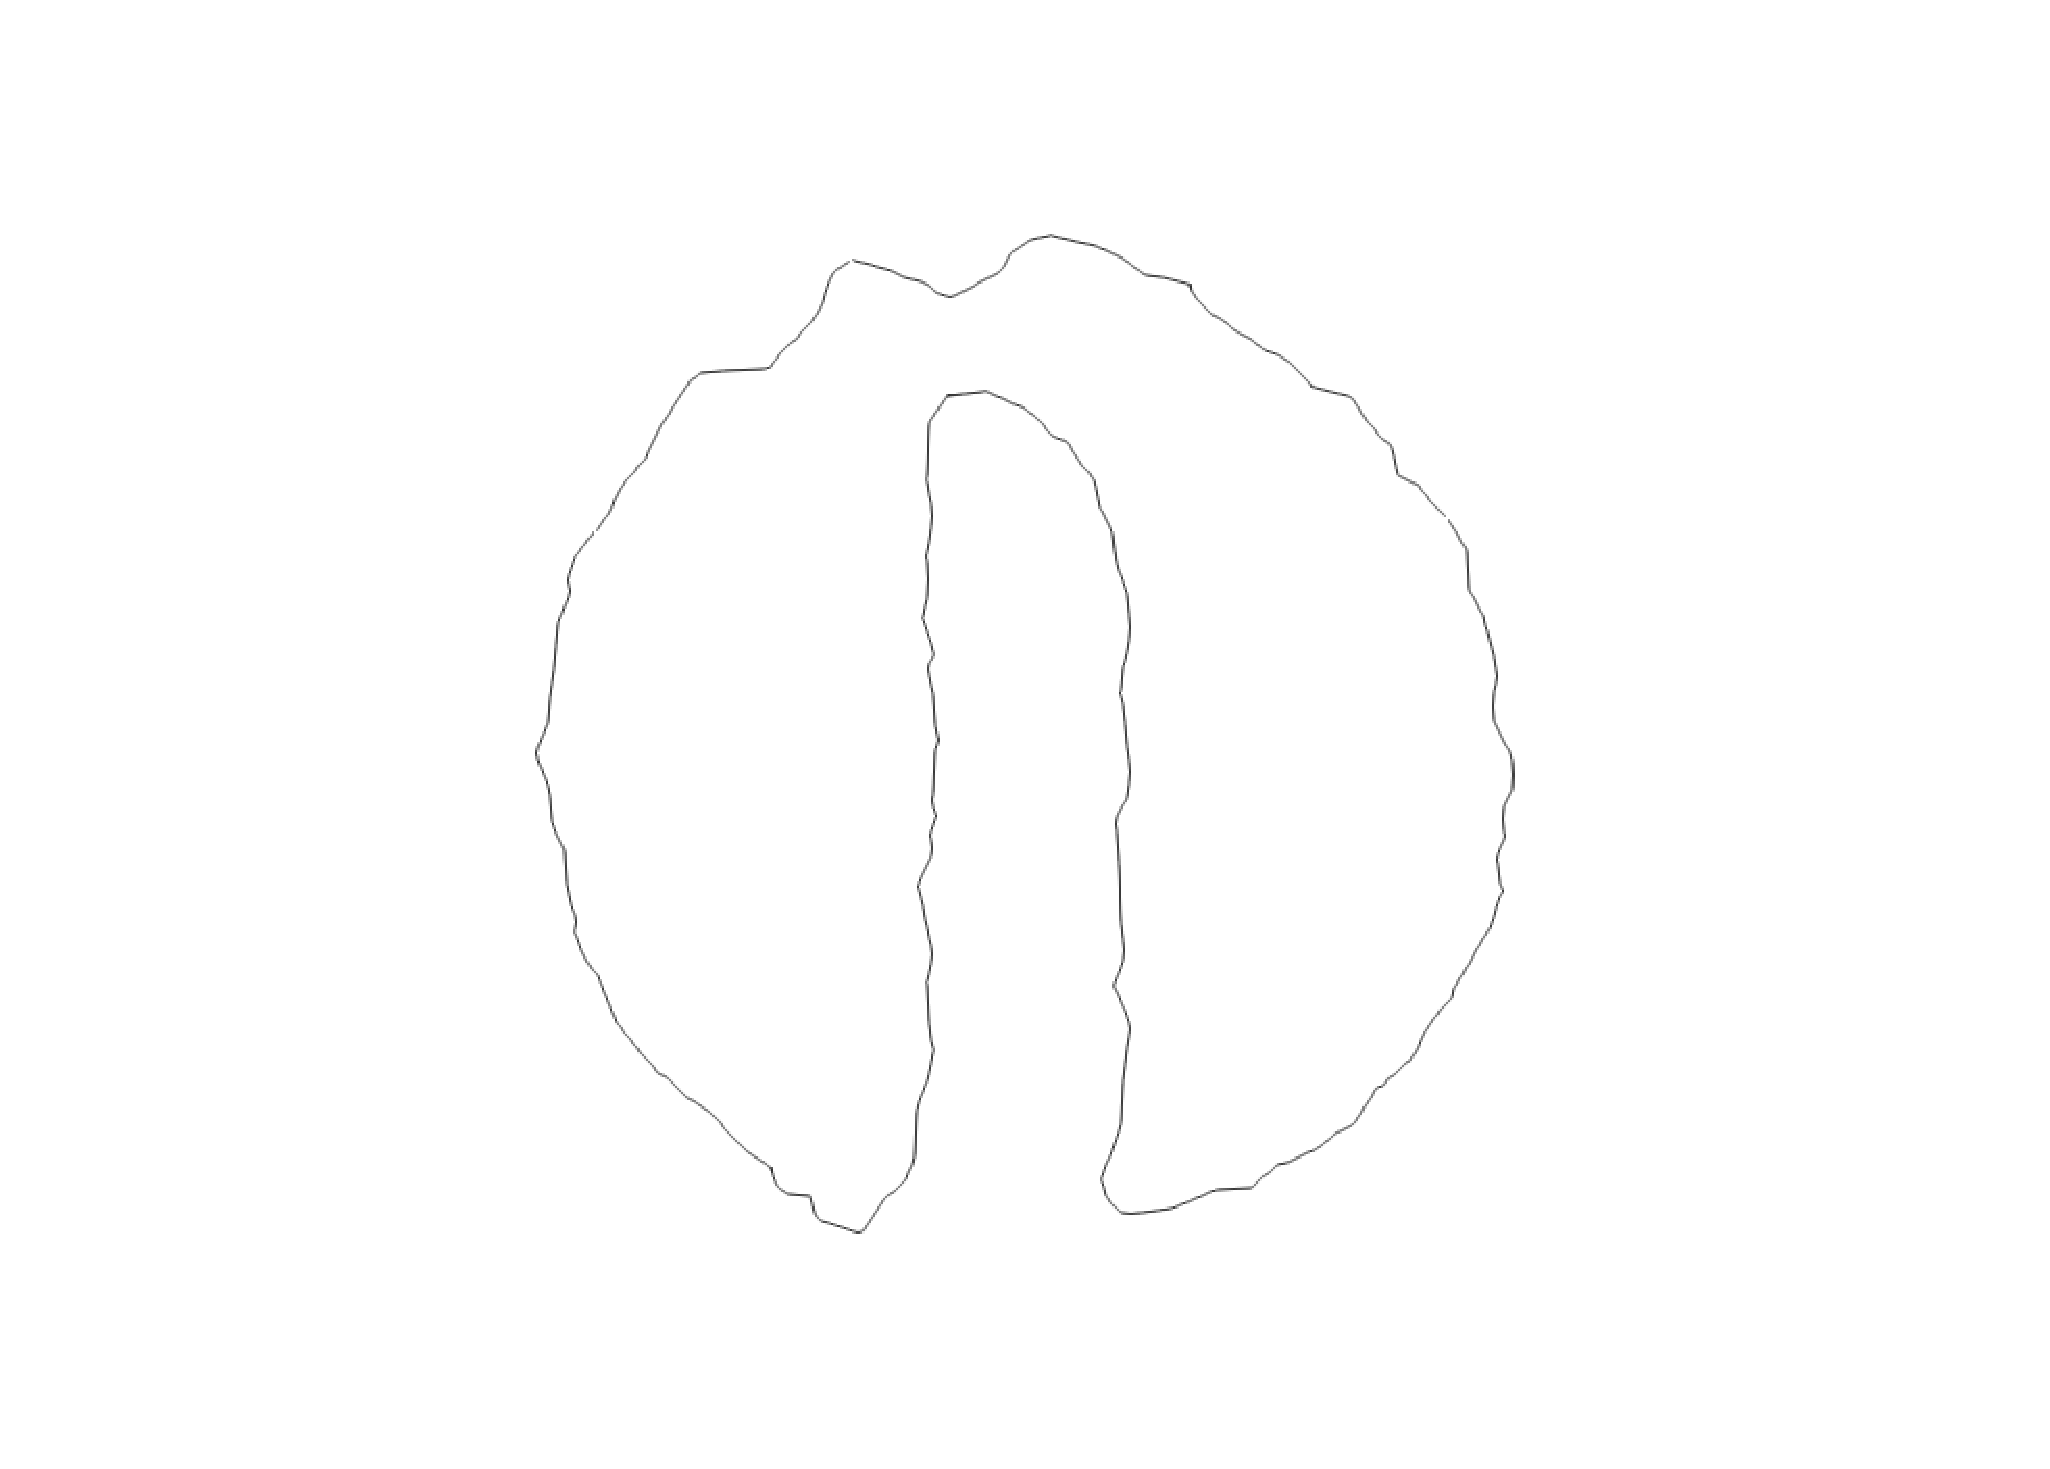
\includegraphics[width=0.3\textwidth]{CLSTriCo01Coarse.eps}
%\caption{fig1}
\label{fig:CLSTriCo01Coarse}
}
\subfigure[]{
\centering
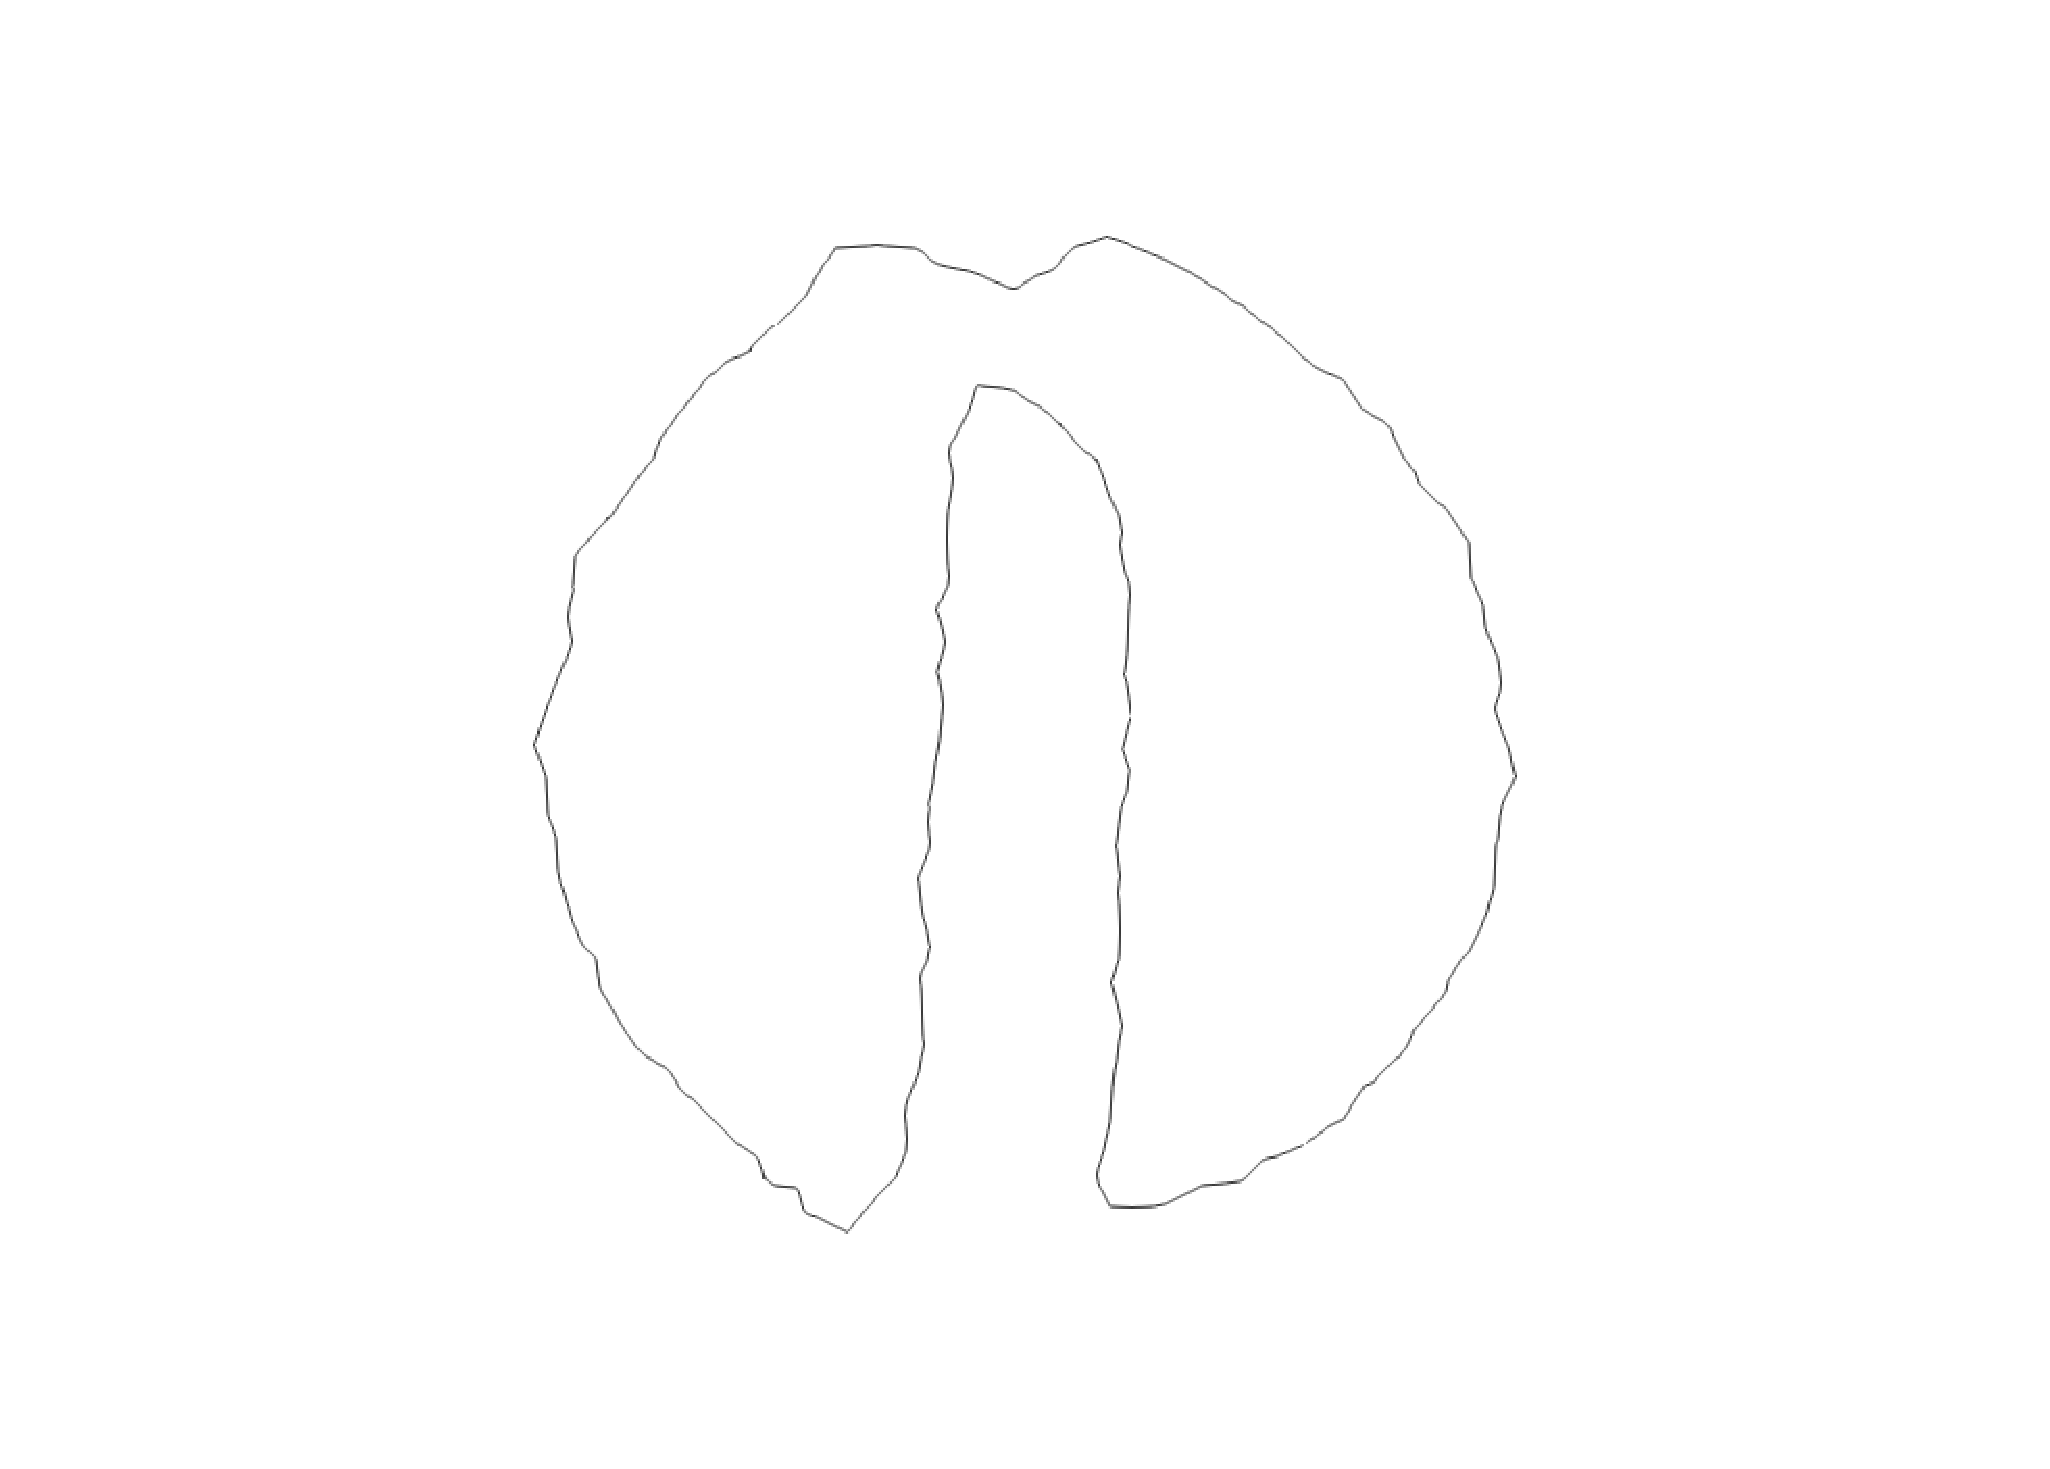
\includegraphics[width=0.3\textwidth]{CLSTriCo05Coarse.eps}
%\caption{fig1}
\label{fig:CLSTriCo05Coarse}
}
\subfigure[]{
\centering
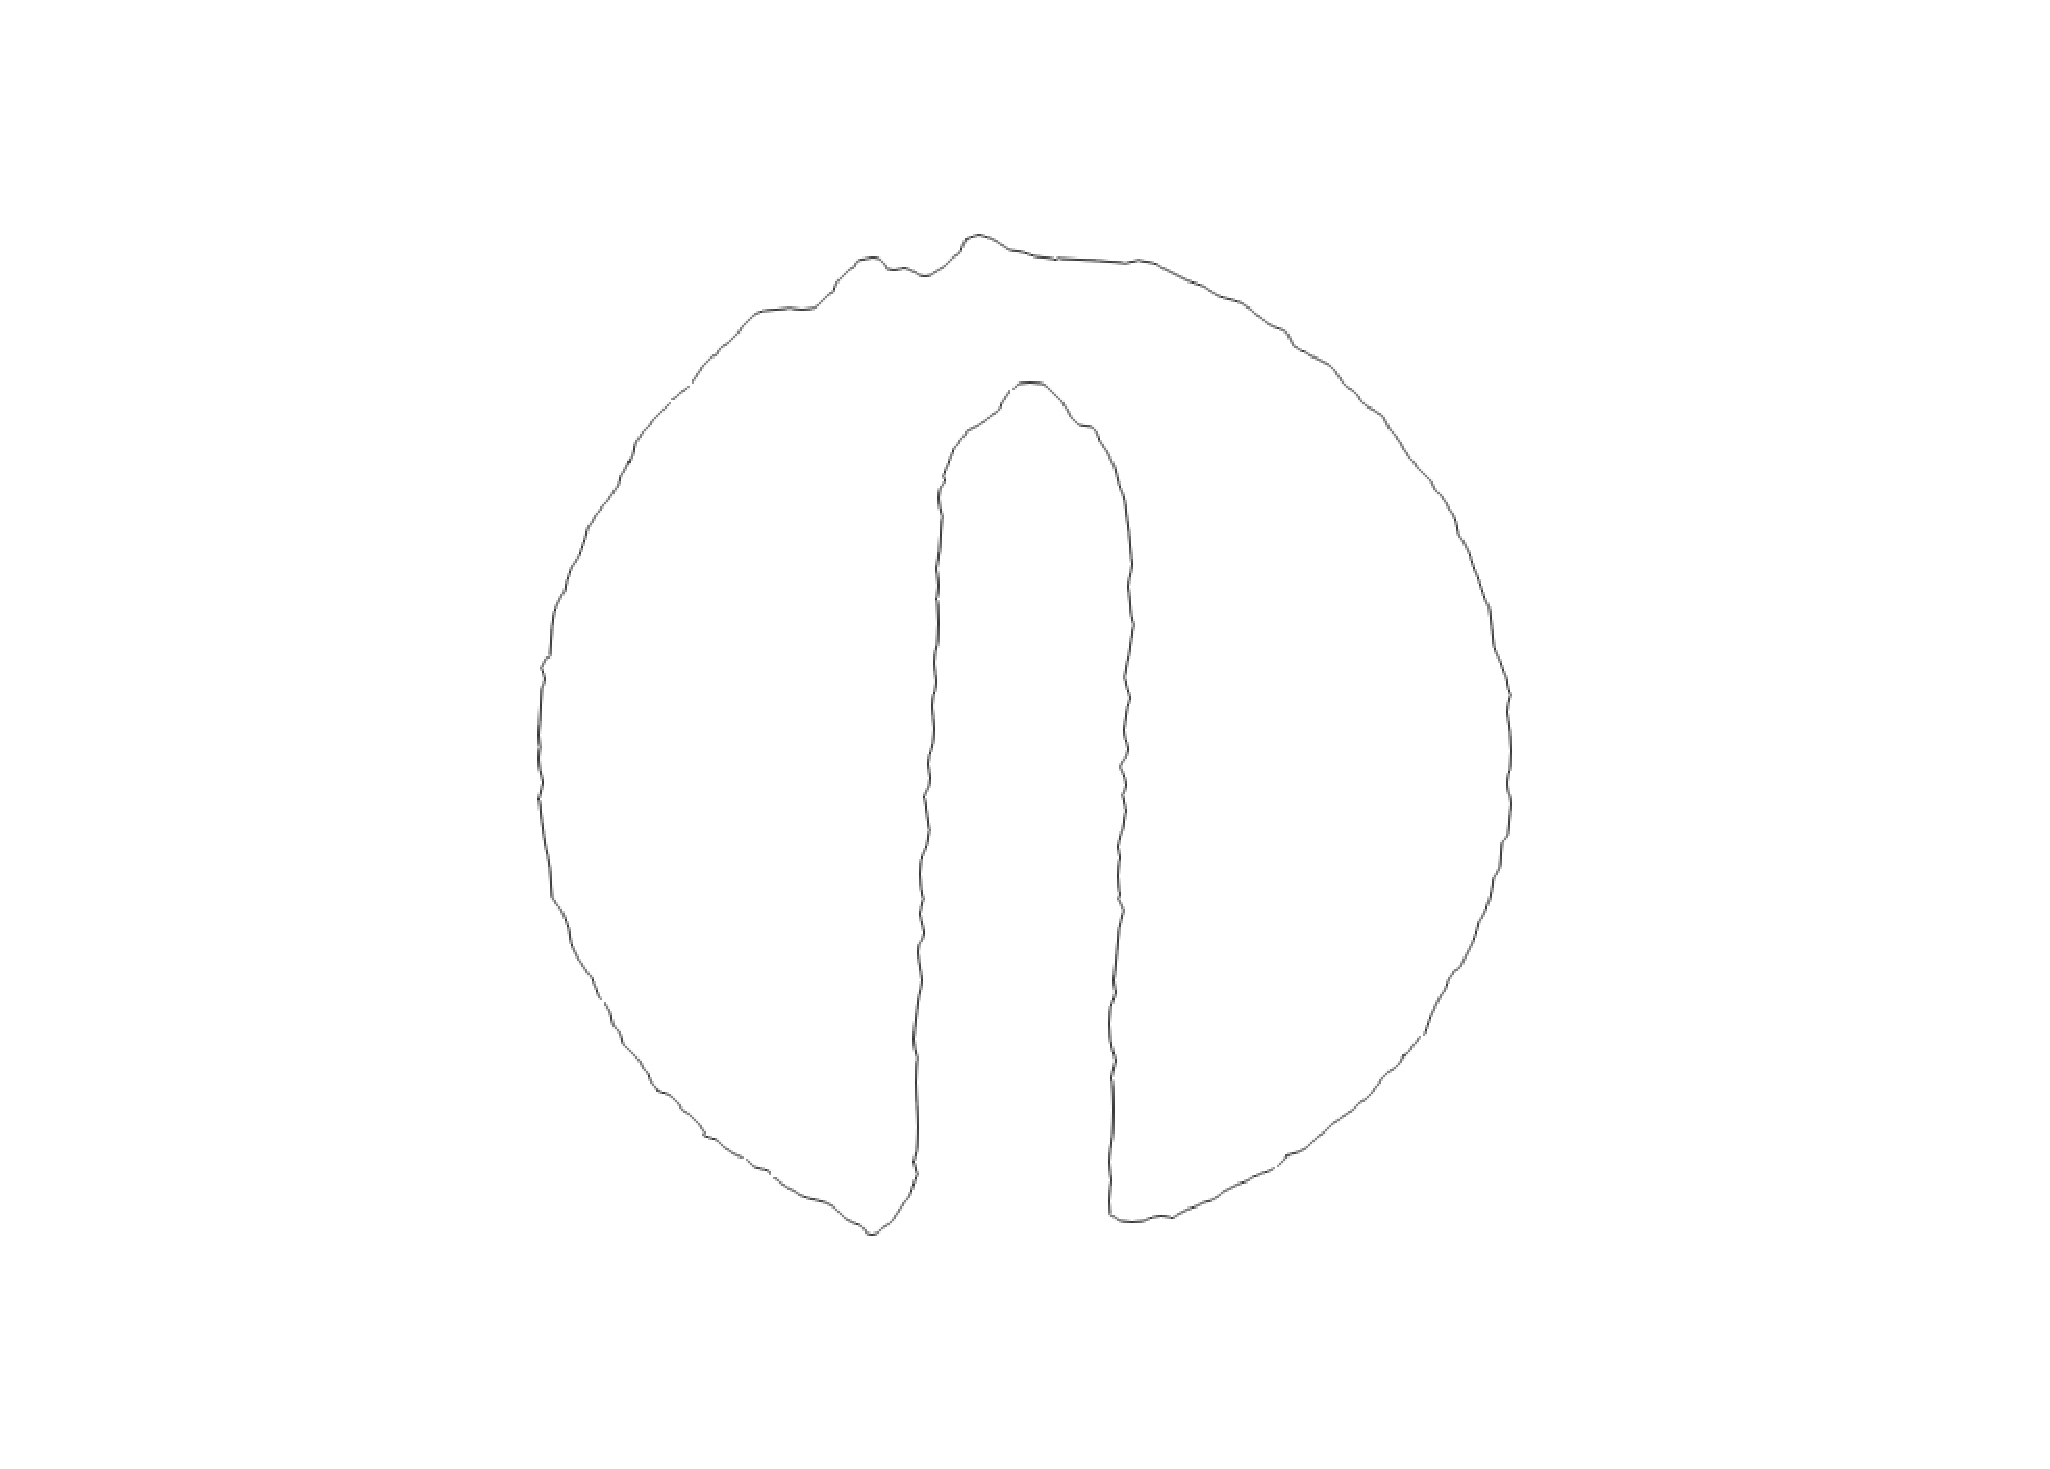
\includegraphics[width=0.3\textwidth]{CLSTriCo05Mid.eps}
\label{fig:CLSTriCo05Mid}
%\caption{fig2}
}
\caption{The shape after one circle with CLSAdvection method:\subref{fig:CLSTriCo01Coarse} 68805 and $Co=0.1$, \subref{fig:CLSTriCo05Coarse} 68805 and $Co=0.5$,\subref{fig:CLSTriCo05Mid} 203965 and $Co=0.5$}
\label{fig:CLSTri}
\end{figure}
%%%%%%%%%%%%%%%%%%%%%%%%%%%%%%%%%%%%%%%%%%%%%%%%%%%%
\begin{figure}[htbp]
\centering
\subfigure[]{
\centering
\includegraphics[width=0.3\textwidth]{MULESHex100.eps}
%\caption{fig1}
\label{fig:MULESHex100}
}
\subfigure[]{
\centering
\includegraphics[width=0.3\textwidth]{ISOHex100.eps}
%\caption{fig1}
\label{fig:ISOHex100}
}
\subfigure[]{
\centering
\includegraphics[width=0.3\textwidth]{CLSHex100.eps}
\label{fig:CLSHex100}
%\caption{fig2}
}
\caption{Spiraling discs at $T=4$ with $Co=0.5$.\subref{MULESHex100}: $100\times{100}$, MULES.\subref{ISOHex100}: $100\times{100}$, isoAdvector.\subref{CLSHex100}: $100\times{100}$.}
\label{fig:SpiralingdiscHex1}
\end{figure}
%%%%%%%%%%%%%%%%%%%%%%%%%%%%%%%%%%%%%%%%%%%%%%%%%%
\begin{figure}[htbp]
\centering
\subfigure[]{
\centering
\includegraphics[width=0.3\textwidth]{MULESHex200.eps}
%\caption{fig1}
\label{fig:MULESHex200}
}
\subfigure[]{
\centering
\includegraphics[width=0.3\textwidth]{ISOHex200.eps}
%\caption{fig1}
\label{fig:ISOHex200}
}
\subfigure[]{
\centering
\includegraphics[width=0.3\textwidth]{CLSHex200.eps}
\label{fig:CLSHex200}
%\caption{fig2}
}
\caption{Spiraling discs at $T=4$ with $Co=0.5$.\subref{MULESHex100}: \subref{MULESHex200}: $200\times{200}$, MULES.\subref{ISOHex100}: $200\times{200}$, isoAdvector.\subref{CLSHex100}: $200\times{200}$, CLSAdvection.}
\label{fig:SpiralingdiscHex2}
\end{figure}
%%%%%%%%%%%%%%%%%%%%%%%%%%%%%%%%%%%%%%%%%%%%%%%%
\begin{figure}[htbp]
\centering
\subfigure[]{
\centering
\includegraphics[width=0.3\textwidth]{MULESHex300.eps}
%\caption{fig1}
\label{fig:MULESHex300}
}
\subfigure[]{
\centering
\includegraphics[width=0.3\textwidth]{ISOHex300.eps}
%\caption{fig1}
\label{fig:ISOHex300}
}
\subfigure[]{
\centering
\includegraphics[width=0.3\textwidth]{CLSHex300.eps}
\label{fig:CLSHex300}
%\caption{fig2}
}
\caption{Spiraling discs at $T=4$ with $Co=0.5$.\subref{MULESHex100}:\subref{MULESHex300}: $300\times{300}$, MULES.\subref{ISOHex300}: $300\times{300}$, isoAdvector.\subref{CLSHex300}: $300\times{300}$, CLSAdvection.}
\label{fig:SpiralingdiscHex3}
\end{figure}
%%%%%%%%%%%%%%%%%%%%%%%%%%%%%%%%%%%%%%%%%%%%%%
\begin{figure}[htbp]
\centering
\subfigure[]{
\centering
\includegraphics[width=0.3\textwidth]{MULESPolyCoarse.eps}
%\caption{fig1}
\label{fig:MULESPolyCoarse}
}
\subfigure[]{
\centering
\includegraphics[width=0.3\textwidth]{ISOPolyCoarse.eps}
%\caption{fig1}
\label{fig:ISOPolyCoarse}
}
\subfigure[]{
\centering
\includegraphics[width=0.3\textwidth]{CLSPolyCoarse.eps}
\label{fig:CLSPolyCoarse}
%\caption{fig2}
}
\caption{Spiraling discs at $T=4$ with $Co=0.5$.\subref{MULESPolyCoarse}: $100\times{100}$, MULES.\subref{ISOPolyCoarse}: $100\times{100}$, isoAdvector.\subref{CLSPolyCoarse}: $100\times{100}$, CLSAdvection.}
\label{fig:SpiralingdiscPoly1}
\end{figure}
%%%%%%%%%%%%%%%%%%%%%%%%%%%%%%%%%%%%%%%%%%%%%%%
\begin{figure}[htbp]
\centering
\subfigure[]{
\centering
\includegraphics[width=0.3\textwidth]{MULESPolyMid.eps}
%\caption{fig1}
\label{fig:MULESPolyMid}
}
\subfigure[]{
\centering
\includegraphics[width=0.3\textwidth]{ISOPolyMid.eps}
%\caption{fig1}
\label{fig:ISOPolyMid}
}
\subfigure[]{
\centering
\includegraphics[width=0.3\textwidth]{CLSPolyMid.eps}
\label{fig:CLSPolyMid}
%\caption{fig2}
}
\caption{Spiraling discs at $T=4$ with $Co=0.5$.\subref{MULESPolyCoarse}: \subref{MULESPolyMid}: $200\times{200}$, MULES.\subref{ISOPolyMid}: $200\times{200}$, isoAdvector.\subref{CLSPolyMid}: $200\times{200}$, CLSAdvection.}
\label{fig:SpiralingdiscPoly2}
\end{figure}
%%%%%%%%%%%%%%%%%%%%%%%%%%%%%%%%%%%%%%%%%%%%%%%%%%%
\begin{figure}[htbp]
\centering
\subfigure[]{
\centering
\includegraphics[width=0.3\textwidth]{MULESPolyFine.eps}
%\caption{fig1}
\label{fig:MULESPolyFine}
}
\subfigure[]{
\centering
\includegraphics[width=0.3\textwidth]{ISOPolyFine.eps}
%\caption{fig1}
\label{fig:ISOPolyFine}
}
\subfigure[]{
\centering
\includegraphics[width=0.3\textwidth]{CLSPolyFine.eps}
\label{fig:CLSPolyFine}
%\caption{fig2}
}
\caption{Spiraling discs at $T=4$ with $Co=0.5$.\subref{MULESPolyCoarse}:\subref{MULESPolyFine}: $300\times{300}$, MULES.\subref{ISOPolyFine}: $300\times{300}$, isoAdvector.\subref{CLSPolyFine}: $FinePoly$, CLSAdvection.}
\label{fig:SpiralingdiscPoly3}
\end{figure}
%%%%%%%%%%%%%%%%%%%%%%%%%%%%%%%%%%%%%%%%%%%%%%%%%%%%%%%%
\begin{figure}[htbp]
\centering
\subfigure[]{
\centering
\includegraphics[width=0.3\textwidth]{MULESTriCoarse.eps}
%\caption{fig1}
\label{fig:MULESTriCoarse}
}
\subfigure[]{
\centering
\includegraphics[width=0.3\textwidth]{ISOTriCoarse.eps}
%\caption{fig1}
\label{fig:ISOTriCoarse}
}
\subfigure[]{
\centering
\includegraphics[width=0.3\textwidth]{CLSTriCoarse.eps}
\label{fig:CLSTriCoarse}
%\caption{fig2}
}
\caption{Spiraling discs at $T=4$ with $Co=0.5$.\subref{MULESTriCoarse}: $100\times{100}$, MULES.\subref{ISOTriCoarse}: $100\times{100}$, isoAdvector.\subref{CLSTriCoarse}: $100\times{100}$, CLSAdvection.}
\label{fig:SpiralingdiscTri1}
\end{figure}
%%%%%%%%%%%%%%%%%%%%%%%%%%%%%%%%%%%%%%%%%%%%%%%%%%%%%%%
\begin{figure}[htbp]
\centering
\subfigure[]{
\centering
\includegraphics[width=0.3\textwidth]{MULESTriMid.eps}
%\caption{fig1}
\label{fig:MULESTriMid}
}
\subfigure[]{
\centering
\includegraphics[width=0.3\textwidth]{ISOTriMid.eps}
%\caption{fig1}
\label{fig:ISOTriMid}
}
\subfigure[]{
\centering
\includegraphics[width=0.3\textwidth]{CLSTriMid.eps}
\label{fig:CLSTriMid}
%\caption{fig2}
}
\caption{Spiraling discs at $T=4$ with $Co=0.5$.\subref{MULESTriMid}: $200\times{200}$, MULES.\subref{ISOTriMid}: $200\times{200}$, isoAdvector.\subref{CLSTriMid}: $200\times{200}$, CLSAdvection.}
\label{fig:SpiralingdiscTri2}
\end{figure}
%%%%%%%%%%%%%%%%%%%%%%%%%%%%%%%%%%%%%%%%%%%%%%%%%%%%%%
\begin{figure}[htbp]
\centering
\subfigure[]{
\centering
\includegraphics[width=0.3\textwidth]{MULESTriFine.eps}
%\caption{fig1}
\label{fig:MULESTriFine}
}
\subfigure[]{
\centering
\includegraphics[width=0.3\textwidth]{ISOTriFine.eps}
%\caption{fig1}
\label{fig:ISOTriFine}
}
\subfigure[]{
\centering
\includegraphics[width=0.3\textwidth]{CLSTriFine.eps}
\label{fig:CLSTriFine}
%\caption{fig2}
}
\caption{Spiraling discs at $T=4$ with $Co=0.5$.\subref{MULESTriFine}: $300\times{300}$, MULES.\subref{ISOTriFine}: $300\times{300}$, isoAdvector.\subref{CLSTriFine}: $FinePoly$, CLSAdvection.}
\label{fig:SpiralingdiscTri3}
\end{figure}
%%%%%%%%%%%%%%%%%Dam Break Mesh Check%%%%%%%%%%%%%%%%%%%%%%%%%%%%%%
\begin{figure}[htbp]
\centering
\subfigure[]{
\centering
\includegraphics[width=0.3\textwidth]{MULES100T085.eps}
%\caption{fig1}
\label{fig:MULES100T085}
}
\subfigure[]{
\centering
\includegraphics[width=0.3\textwidth]{ISO100T085.eps}
%\caption{fig1}
\label{fig:ISO100T085}
}
\subfigure[]{
\centering
\includegraphics[width=0.3\textwidth]{CLS100T085.eps}
\label{fig:CLS100T085}
%\caption{fig2}
}
\caption{Check the mesh sensitivity of dam break case with different methods at time $T =1s$.\subref{fig:MULES100T085}: mesh size $100\times{100}$, MULES.\subref{fig:ISO100T085}: mesh size $100\times{100}$, isoAdvector. \subref{fig:CLS100T085}: mesh size $100\times{100}$.}
\label{fig:DamBreakMeshSensitivity1}
\end{figure}
%%%%%%%%%%%%%%%%%%%%%%%%%%%%%%%%%%%%%%%%%%%%%%%%%%%%%%%%%%%%%%%%%%%%%%%%%%%%%%
\begin{figure}[htbp]
\centering
\subfigure[]{
\centering
\includegraphics[width=0.3\textwidth]{MULES200T085.eps}
%\caption{fig1}
\label{fig:MULES200T085}
}
\subfigure[]{
\centering
\includegraphics[width=0.3\textwidth]{ISO200T085.eps}
%\caption{fig1}
\label{fig:ISO200T085}
}
\subfigure[]{
\centering
\includegraphics[width=0.3\textwidth]{CLS200T085.eps}
\label{fig:CLS200T085}
%\caption{fig2}
}
\caption{Check the mesh sensitivity of dam break case with different methods at time $T =1s$. \subref{fig:MULES200T085}: mesh size $200\times{200}$, MULES.\subref{fig:ISO200T085}: mesh size $200\times{200}$, isoAdvector. \subref{fig:CLS200T085}: mesh size $200\times{200}$, CLSAdvection.}
\label{fig:DamBreakMeshSensitivity2}
\end{figure}
%%%%%%%%%%%%%%%%%%%%%%%%%%%%%%%%%%%%%%%%%%%%%%%%%%%%%%%%%%%%%%%%
\begin{figure}[htbp]
\centering
\subfigure[]{
\centering
\includegraphics[width=0.3\textwidth]{MULES300T085.eps}
%\caption{fig1}
\label{fig:MULES300T085}
}
\subfigure[]{
\centering
\includegraphics[width=0.3\textwidth]{ISO300T085.eps}
%\caption{fig1}
\label{fig:ISO300T085}
}
\subfigure[]{
\centering
\includegraphics[width=0.3\textwidth]{CLS300T085.eps}
\label{fig:CLS300T085}
%\caption{fig2}
}
\caption{Check the mesh sensitivity of dam break case with different methods at time $T =1s$.\subref{fig:MULES100T085}:\subref{fig:MULES300T085}: mesh size $300\times{300}$, MULES.\subref{fig:ISO300T085}: mesh size $300\times{300}$, isoAdvector. \subref{fig:CLS300T085}: mesh size $300\times{300}$, CLSAdvection.}
\label{fig:DamBreakMeshSensitivity3}
\end{figure}
%%%%%%%%%%%%%%%%%%%%%%%%%%%%%%%%%%%%%%%%%%%%%%%%%%%%%%%%%%
\begin{figure}[htbp]
\centering
\subfigure[]{
\centering
\includegraphics[width=0.3\textwidth]{MULES300T010.eps}
%\caption{fig1}
\label{fig:MULES300T010}
}
\subfigure[]{
\centering
\includegraphics[width=0.3\textwidth]{ISO300T010.eps}
%\caption{fig1}
\label{fig:IS0300T010}
}
\subfigure[]{
\centering
\includegraphics[width=0.3\textwidth]{CLS300T010.eps}
\label{fig:CLS300T010}
}
\caption{Dam break with different algorithm.}
\label{fig:DamBreak01}
\end{figure}
%%%%%%%%%%%%%%%%%%%%%%%%%%%%%%%%%%%%%%%%%%%%%%%%%%%%%%%
\begin{figure}[htbp]
\centering
\subfigure[]{
\centering
\includegraphics[width=0.3\textwidth]{MULES300T020.eps}
%\caption{fig1}
\label{fig:MULES300T020}
}
\subfigure[]{
\centering
\includegraphics[width=0.3\textwidth]{ISO300T020.eps}
%\caption{fig1}
\label{fig:IS0300T020}
}
\subfigure[]{
\centering
\includegraphics[width=0.3\textwidth]{CLS300T020.eps}
\label{fig:CLS300T020}
}
\caption{Dam break with different algorithm.}
\label{fig:DamBreak02}
\end{figure}
%%%%%%%%%%%%%%%%%%%%%%%%%%%%%%%%%%%%%%%%%%%%%%%%%%%
\begin{figure}[htbp]
\centering
\subfigure[]{
\centering
\includegraphics[width=0.3\textwidth]{MULES300T030.eps}
%\caption{fig1}
\label{fig:MULES300T030}
}
\subfigure[]{
\centering
\includegraphics[width=0.3\textwidth]{ISO300T030.eps}
%\caption{fig1}
\label{fig:IS0300T030}
}
\subfigure[]{
\centering
\includegraphics[width=0.3\textwidth]{CLS300T030.eps}
\label{fig:CLS300T030}
}
\caption{Dam break with different algorithm.}
\label{fig:DamBreak03}
\end{figure}
%%%%%%%%%%%%%%%%%%%%%%%%%%%%%%%%%%%%%%%%%%%%%%%%%%%
\begin{figure}[htbp]
\centering
\subfigure[]{
\centering
\includegraphics[width=0.3\textwidth]{MULES300T040.eps}
%\caption{fig1}
\label{fig:MULES300T040}
}
\subfigure[]{
\centering
\includegraphics[width=0.3\textwidth]{ISO300T040.eps}
%\caption{fig1}
\label{fig:IS0300T040}
}
\subfigure[]{
\centering
\includegraphics[width=0.3\textwidth]{CLS300T040.eps}
\label{fig:CLS300T040}
}
\caption{Dam break with different algorithm.}
\label{fig:DamBreak04}
\end{figure}
%%%%%%%%%%%%%%%%%%%%%%%%%%%%%%%%%%%%%%%%%%%%%%%%%%
\begin{figure}[htbp]
\centering
\subfigure[]{
\centering
\includegraphics[width=0.3\textwidth]{MULES300T050.eps}
%\caption{fig1}
\label{fig:MULES300T050}
}
\subfigure[]{
\centering
\includegraphics[width=0.3\textwidth]{ISO300T050.eps}
%\caption{fig1}
\label{fig:ISO300T050}
}
\subfigure[]{
\centering
\includegraphics[width=0.3\textwidth]{CLS300T050.eps}
\label{fig:CLS300T050}
}
\caption{Dam break with different algorithm.}
\label{fig:DamBreak05}
\end{figure}
%%%%%%%%%%%%%%%%%%%%%%%%%%%%%%%%%%%%%%%%%%%%%%%%%%
\begin{figure}[htbp]
\centering
\subfigure[]{
\centering
\includegraphics[width=0.3\textwidth]{MULES300T060.eps}
%\caption{fig1}
\label{fig:MULES300T060}
}
\subfigure[]{
\centering
\includegraphics[width=0.3\textwidth]{ISO300T060.eps}
%\caption{fig1}
\label{fig:IS0300T060}
}
\subfigure[]{
\centering
\includegraphics[width=0.3\textwidth]{CLS300T060.eps}
\label{fig:CLS300T060}
}
\caption{Dam break with different algorithm.}
\label{fig:DamBreak06}
\end{figure}
%%%%%%%%%%%%%%%%%%%%%%%%%%%%%%%%%%%%%%%%%%%%%%%%
\begin{figure}[htbp]
\centering
\subfigure[]{
\centering
\includegraphics[width=0.3\textwidth]{MULES300T070.eps}
%\caption{fig1}
\label{fig:MULES300T070}
}
\subfigure[]{
\centering
\includegraphics[width=0.3\textwidth]{ISO300T070.eps}
%\caption{fig1}
\label{fig:IS0300T070}
}
\subfigure[]{
\centering
\includegraphics[width=0.3\textwidth]{CLS300T070.eps}
\label{fig:CLS300T070}
}
\caption{Dam break with different algorithm.}
\label{fig:DamBreak07}
\end{figure}
%%%%%%%%%%%%%%%%%%%%%%%%%%%%%%%%%%%%%%%%%%%%%%%
\begin{figure}[htbp]
\centering
\subfigure[]{
\centering
\includegraphics[width=0.3\textwidth]{MULES300T080.eps}
%\caption{fig1}
\label{fig:MULES300T080}
}
\subfigure[]{
\centering
\includegraphics[width=0.3\textwidth]{ISO300T080.eps}
%\caption{fig1}
\label{fig:IS0300T080}
}
\subfigure[]{
\centering
\includegraphics[width=0.3\textwidth]{CLS300T080.eps}
\label{fig:CLS300T080}
}
\caption{Dam break with different algorithm.}
\label{fig:DamBreak08}
\end{figure}
%%%%%%%%%%%%%%%%%%%%%%%%%%%%%%%%%%%%%%%%%%%%%%%%%
\begin{figure}[htbp]
\centering
\subfigure[]{
\centering
\includegraphics[width=0.3\textwidth]{MULES300T090.eps}
%\caption{fig1}
\label{fig:MULES300T090}
}
\subfigure[]{
\centering
\includegraphics[width=0.3\textwidth]{ISO300T090.eps}
%\caption{fig1}
\label{fig:IS0300T090}
}
\subfigure[]{
\centering
\includegraphics[width=0.3\textwidth]{CLS300T090.eps}
\label{fig:CLS300T090}
}
\caption{Dam break with different algorithm.}
\label{fig:DamBreak09}
\end{figure}
%%%%%%%%%%%%%%%%%%%%%%%%%%%%%%%%%%%%%%%%%%%%%%%%%%%
\begin{figure}[htbp]
\centering
\subfigure[]{
\centering
\includegraphics[width=0.3\textwidth]{MULES300T100.eps}
%\caption{fig1}
\label{fig:MULES300T100}
}
\subfigure[]{
\centering
\includegraphics[width=0.3\textwidth]{ISO300T100.eps}
%\caption{fig1}
\label{fig:IS0300T100}
}
\subfigure[]{
\centering
\includegraphics[width=0.3\textwidth]{CLS300T100.eps}
\label{fig:CLS300T100}
}
%\caption{fig2}
\caption{Dam break with different algorithm.}
\label{fig:DamBreak10}
\end{figure}
%%%%%%%%%%%%%%%%%%%%%%%%%%%%%%%%%%%%%%%%%%%%%%%%%%%%%%
\begin{table}
\centering
\caption{Errors and calculation times for hex meshes of notched disc}
\label{Tab:01}
\begin{tabular}{ccccc}
\hline\noalign{\smallskip}
\quad &(N,Co) & MULES &isoAdvector &CLSAdvection  \\
\noalign{\smallskip}\hline\noalign{\smallskip}
\multirow{5}{*}{$\varepsilon_{V}$}
&(100,0.1)& 1.06e-06 &6.36e-11 &7.57e-11  \\
&(100,0.2) & 4.79e-07 &3.55e-10 &1.65e-10\\
&(100,0.5)& 5.67e-07 &1.75e-07 &4.10e-08\\
&(200,0.5) & 4.88e-07 &1.67e-06 &6.92e-07\\
&(400,0.5) & 3.33e-07 &8.55e-07 &3.97e-06\\
\hline\noalign{\smallskip}
\multirow{5}{*}{$\varepsilon_{M}$}
&(100,0.1)& 1.00 &1.00 &0.99  \\
&(100,0.2) & 1.00 &1.00 &0.99\\
&(100,0.5)& 1.00 &1.00 &0.99\\
&(200,0.5) & 1.00 &1.00 &0.99\\
&(400,0.5) & 1.00 &1.00 &1.00\\
\hline\noalign{\smallskip}
\multirow{5}{*}{$\varepsilon_{S}$}
&(100,0.1)& 0.34 &0.13 &0.13  \\
&(100,0.2) & 0.34 &0.13 &0.13\\
&(100,0.5)& 0.37 &0.13 &0.14\\
&(200,0.5) & 0.22 &0.061 &0.065\\
&(400,0.5) & 0.16 &0.027 &0.029\\
\hline\noalign{\smallskip}
\multirow{5}{*}{$\min(\alpha)$}
&(100,0.1)& -2.45e-36 &0 &0  \\
&(100,0.2) & -8.03e-29 &0 &0\\
&(100,0.5)& -6.31e-20 &0 &0\\
&(200,0.5) & -4.40e-29 &0 &0\\
&(400,0.5) & -4.51e-47 &0 &0\\
\hline\noalign{\smallskip}
\multirow{5}{*}{$\max(\alpha)-1$}
&(100,0.1)& -2.90e-06 &0 &0  \\
&(100,0.2) & -1.29e-05 &0 &0 \\
&(100,0.5)& -12.97e-04 &0 &0\\
&(200,0.5) & -2.49e-08 &0 &0\\
&(400,0.5) & -1.26e-10 &0 &0\\
\hline\noalign{\smallskip}
\multirow{5}{*}{$T_{calc}$}
&(100,0.1)& 1160 &417 &1489  \\
&(100,0.2) & 648 &390 &873\\
&(100,0.5)& 97 &148 &424\\
&(200,0.5) & 2373 &1461 &2867\\
&(400,0.5) & 7268 &7214 &12500\\
\noalign{\smallskip}\hline
\end{tabular}
\end{table}
%%%%%%%%%%%%%%%%%%%%%%%%%%%%%%%%%%%%%%%%%%
\begin{table}
\centering
\caption{Errors and calculation times for polygon meshes of notched disc}
\label{Tab:02}
\begin{tabular}{ccccc}
\hline\noalign{\smallskip}
\quad &(Cell Numbers,Co) & MULES &isoAdvector &CLSAdvection  \\
\noalign{\smallskip}\hline\noalign{\smallskip}
\multirow{5}{*}{$\varepsilon_{V}$}
&(51967,0.1)& 9.30e-09 &1.12e-10 &1.14e-10  \\
&(51967,0.5) & 7.37e-07 &4.05e-11 &4.03e-11\\
&(203965,0.5)& 2.77e-06 &2.74e-11 &2.94e-11\\
\hline\noalign{\smallskip}
\multirow{5}{*}{$\varepsilon_{M}$}
&(51967,0.1)& 1.00 &1.00 &1.00  \\
&(51967,0.5) & 1.00 &1.00 &1.00\\
&(203965,0.5)& 1.00 &1.00 &1.00\\
\hline\noalign{\smallskip}
\multirow{5}{*}{$\varepsilon_{S}$}
&(51967,0.1)& 0.39 &0.14 &0.14  \\
&(51967,0.5) & 0.39 &0.14 &0.15\\
&(203965,0.5)& 0.20 &0.071 &0.071\\
\hline\noalign{\smallskip}
\multirow{5}{*}{$\min(\alpha)$}
&(51967,0.1)& -8.22e-11 &0 &0  \\
&(51967,0.5) & -2.54e-06 &0 &0\\
&(203965,0.5)& -7.72e-06 &0 &0\\
\hline\noalign{\smallskip}
\multirow{5}{*}{$\max(\alpha)-1$}
&(51967,0.1)& -8.92e-06 &0 &0  \\
&(51967,0.5) & -7.37e-05 &0 &0\\
&(203965,0.5)& 1.44e-05 &0 &0\\
\hline\noalign{\smallskip}
\multirow{5}{*}{$T_{calc}$}
&(51967,0.1)& 3170 &803 &1850  \\
&(51967,0.5) & 289 &511 &368\\
&(203965,0.5)& 2521 &1512 &3550\\
\noalign{\smallskip}\hline
\end{tabular}
\end{table}
%%%%%%%%%%%%%%%%%%%%%%%%%%%%%%%%%%%%%%%%%%%%%%%%%%%%%%%
\begin{table}
\centering
\caption{Errors and calculation times for triangle meshes of notched disc}
\label{Tab:03}
\begin{tabular}{ccccc}
\hline\noalign{\smallskip}
\quad &(Cell Numbers, Co) & MULES &isoAdvector &CLSAdvection  \\
\noalign{\smallskip}\hline\noalign{\smallskip}
\multirow{5}{*}{$\varepsilon_{V}$}
&(68805,0.1)& 2.58e-07 &5.22e-11 &1.53e-05  \\
&(68805,0.5) & 9.93e-07 &7.39e-10 &1.30e-05\\
&(277605,0.5)& 2.24e-07 &7.60e-09 &6.85e-06\\
\hline\noalign{\smallskip}
\multirow{5}{*}{$\varepsilon_{M}$}
&(68805,0.1)& 1.00 &1.00 &1.00  \\
&(68805,0.5) & 1.00 &1.00 &1.00\\
&(277605,0.5)& 1.00 &1.00 &1.00\\
\hline\noalign{\smallskip}
\multirow{5}{*}{$\varepsilon_{S}$}
&(68805,0.1)& 0.44 &0.11 &0.15  \\
&(68805,0.5) & 0.47 &0.12 &0.32\\
&(277605,0.5)& 0.30 &0.062 &0.30\\
\hline\noalign{\smallskip}
\multirow{5}{*}{$\min(\alpha)$}
&(68805,0.1)& -2.97e-24 &0 &0  \\
&(68805,0.5) & -1.03e-17 &0 &0\\
&(277605,0.5)& -3.76e-18 &0 &0\\
\hline\noalign{\smallskip}
\multirow{5}{*}{$\max(\alpha)-1$}
&(68805,0.1)& -1.36e-04 &0 &0  \\
&(68805,0.5) & -4.41e-04 &0 &0\\
&(277605,0.5)& -3.10e-06 &0 &0\\
\hline\noalign{\smallskip}
\multirow{5}{*}{$T_{calc}$}
&(68805,0.1)& 5446 &1904 &7102  \\
&(68805,0.5) & 670 &1055 &1900\\
&(277605,0.5)& 5632 &3474 &11100\\
\noalign{\smallskip}\hline
\end{tabular}
\end{table}
%%%%%%%%%%%%%%%Hex%%%%%%%%%%%%%%%%%%%%%%%%%%%%%%%
\begin{table}
\centering
\caption{Errors and calculation times for structured meshes of spiraling disc}
\label{Tab:04}
\begin{tabular}{ccccc}
\hline\noalign{\smallskip}
\quad &(Mesh size) & MULES &isoAdvector &CLSAdvection  \\
\noalign{\smallskip}\hline\noalign{\smallskip}
\multirow{5}{*}{$\varepsilon_{V}$}
&($100\times{100}$)& 2.58e-07 &5.22e-11 &1.53e-05  \\
&($200\times{200}$) & 9.93e-07 &7.39e-10 &1.30e-05\\
&($300\times{300}$)& 2.24e-07 &7.60e-09 &6.85e-06\\
\hline\noalign{\smallskip}
\multirow{5}{*}{$\varepsilon_{M}$}
&($100\times{100}$)& 2.58e-07 &5.22e-11 &1.53e-05  \\
&($200\times{200}$) & 9.93e-07 &7.39e-10 &1.30e-05\\
&($300\times{300}$)& 2.24e-07 &7.60e-09 &6.85e-06\\
\hline\noalign{\smallskip}
\multirow{5}{*}{$\varepsilon_{S}$}
&($100\times{100}$)& 2.58e-07 &5.22e-11 &1.53e-05  \\
&($200\times{200}$) & 9.93e-07 &7.39e-10 &1.30e-05\\
&($300\times{300}$)& 2.24e-07 &7.60e-09 &6.85e-06\\
\hline\noalign{\smallskip}
\multirow{5}{*}{$\min(\alpha)$}
&($100\times{100}$)& 2.58e-07 &5.22e-11 &1.53e-05  \\
&($200\times{200}$) & 9.93e-07 &7.39e-10 &1.30e-05\\
&($300\times{300}$)& 2.24e-07 &7.60e-09 &6.85e-06\\
\hline\noalign{\smallskip}
\multirow{5}{*}{$\max(\alpha)-1$}
&($100\times{100}$)& 2.58e-07 &5.22e-11 &1.53e-05  \\
&($200\times{200}$) & 9.93e-07 &7.39e-10 &1.30e-05\\
&($300\times{300}$)& 2.24e-07 &7.60e-09 &6.85e-06\\
\hline\noalign{\smallskip}
\multirow{5}{*}{$T_{calc}$}
&($100\times{100}$)& 2.58e-07 &5.22e-11 &1.53e-05  \\
&($200\times{200}$) & 9.93e-07 &7.39e-10 &1.30e-05\\
&($300\times{300}$)& 2.24e-07 &7.60e-09 &6.85e-06\\
\noalign{\smallskip}\hline
\end{tabular}
\end{table}
%%%%%%%%%%%%%%%%%%%%%%%%%%%%%%%%%%%%%%%%%%%%%%%%%%%
\begin{table}
\centering
\caption{Errors and calculation times for polygon meshes of spiraling disc}
\label{Tab:05}
\begin{tabular}{ccccc}
\hline\noalign{\smallskip}
\quad &(Mesh size) & MULES &isoAdvector &CLSAdvection  \\
\noalign{\smallskip}\hline\noalign{\smallskip}
\multirow{5}{*}{$\varepsilon_{V}$}
&(68805,0.1)& 2.58e-07 &5.22e-11 &1.53e-05  \\
&(68805,0.5) & 9.93e-07 &7.39e-10 &1.30e-05\\
&(277605,0.5)& 2.24e-07 &7.60e-09 &6.85e-06\\
\hline\noalign{\smallskip}
\multirow{5}{*}{$\varepsilon_{M}$}
&(68805,0.1)& 1.00 &1.00 &1.00  \\
&(68805,0.5) & 1.00 &1.00 &1.00\\
&(277605,0.5)& 1.00 &1.00 &1.00\\
\hline\noalign{\smallskip}
\multirow{5}{*}{$\varepsilon_{S}$}
&(68805,0.1)& 0.44 &0.11 &0.15  \\
&(68805,0.5) & 0.47 &0.12 &0.32\\
&(277605,0.5)& 0.30 &0.062 &0.30\\
\hline\noalign{\smallskip}
\multirow{5}{*}{$\min(\alpha)$}
&(68805,0.1)& -2.97e-24 &0 &0  \\
&(68805,0.5) & -1.03e-17 &0 &0\\
&(277605,0.5)& -3.76e-18 &0 &0\\
\hline\noalign{\smallskip}
\multirow{5}{*}{$\max(\alpha)-1$}
&(68805,0.1)& -1.36e-04 &0 &0  \\
&(68805,0.5) & -4.41e-04 &0 &0\\
&(277605,0.5)& -3.10e-06 &0 &0\\
\hline\noalign{\smallskip}
\multirow{5}{*}{$T_{calc}$}
&(68805,0.1)& 5446 &1904 &7102  \\
&(68805,0.5) & 670 &1055 &1900\\
&(277605,0.5)& 5632 &3474 &11100\\
\noalign{\smallskip}\hline
\end{tabular}
\end{table}
%%%%%%%%%%%%%%%%%%%%%%%%%%%%%%%%%%%%%%%%%%%%%
\begin{table}
\centering
\caption{Errors and calculation times for triangle meshes of spiraling disc}
\label{Tab:06}
\begin{tabular}{ccccc}
\hline\noalign{\smallskip}
\quad &(Mesh size) & MULES &isoAdvector &CLSAdvection  \\
\noalign{\smallskip}\hline\noalign{\smallskip}
\multirow{5}{*}{$\varepsilon_{V}$}
&(68805,0.1)& 2.58e-07 &5.22e-11 &1.53e-05  \\
&(68805,0.5) & 9.93e-07 &7.39e-10 &1.30e-05\\
&(277605,0.5)& 2.24e-07 &7.60e-09 &6.85e-06\\
\hline\noalign{\smallskip}
\multirow{5}{*}{$\varepsilon_{M}$}
&(68805,0.1)& 1.00 &1.00 &1.00  \\
&(68805,0.5) & 1.00 &1.00 &1.00\\
&(277605,0.5)& 1.00 &1.00 &1.00\\
\hline\noalign{\smallskip}
\multirow{5}{*}{$\varepsilon_{S}$}
&(68805,0.1)& 0.44 &0.11 &0.15  \\
&(68805,0.5) & 0.47 &0.12 &0.32\\
&(277605,0.5)& 0.30 &0.062 &0.30\\
\hline\noalign{\smallskip}
\multirow{5}{*}{$\min(\alpha)$}
&(68805,0.1)& -2.97e-24 &0 &0  \\
&(68805,0.5) & -1.03e-17 &0 &0\\
&(277605,0.5)& -3.76e-18 &0 &0\\
\hline\noalign{\smallskip}
\multirow{5}{*}{$\max(\alpha)-1$}
&(68805,0.1)& -1.36e-04 &0 &0  \\
&(68805,0.5) & -4.41e-04 &0 &0\\
&(277605,0.5)& -3.10e-06 &0 &0\\
\hline\noalign{\smallskip}
\multirow{5}{*}{$T_{calc}$}
&(68805,0.1)& 5446 &1904 &7102  \\
&(68805,0.5) & 670 &1055 &1900\\
&(277605,0.5)& 5632 &3474 &11100\\
\noalign{\smallskip}\hline
\end{tabular}
\end{table}
%%%%%%%%%%%%%%%%%%%%%%%%%%%%%%%%%%%%%%%%
